% % % % % % % % % % % % % % % % % % % % % % % % % % % % % % % % % % % % % % % % % % % %
%                                                                                     %
% Short Sectioned Assignment LaTeX Template Version 1.0 (5/5/12)                      %
% This template has been downloaded from: http://www.LaTeXTemplates.com               %
%                                                                                     %
% Original author:  Frits Wenneker (http://www.howtotex.com)                          %
%                                                                                     %
% Modified by: Fco Javier Sueza Rodríguez (fcosueza@disroot.org)                      %
%                                                                                     %
% Changes:                                                                            %
%	    - Custom Chapters, Sections and Subsections (titlesec package)                %
%           - Document type scrbook (oneside)                                         %
%           - Use babel-lang-spanish package and marvosym                             %
%           - Use hyperref, enumitem, tcolorbox and glossaries packages               %
%           - Use Time New Roman (mathptmx), Helvetic and Courier fonts               %
%                                                                                     %
% License: CC BY-NC-SA 3.0 (http://creativecommons.org/licenses/by-nc-sa/3.0/)        %
%                                                                                     %
% % % % % % % % % % % % % % % % % % % % % % % % % % % % % % % % % % % % % % % % % % % %

%-----------------------------------------------%
%	              Packages                  %
%-----------------------------------------------%

\documentclass[paper=a4, fontsize=11pt, oneside]{scrbook}

% ---- Text Input/Output ----- %

\usepackage[T1]{fontenc}
\usepackage[utf8]{inputenc}
\usepackage{mathptmx}
\usepackage[scaled=.92]{helvet}
\usepackage{courier}
\usepackage[indent=12pt]{parskip}

\usepackage{geometry}
\geometry{verbose,tmargin=3cm,bmargin=3cm,lmargin=2.6cm,rmargin=2.6cm}

% ---- Language ----- %

\usepackage[spanish]{babel}
\usepackage{marvosym}

% ---- Another packages ---- %

\usepackage{amsmath,amsfonts,amsthm}
\usepackage{graphics,graphicx}
\usepackage{titlesec}
\usepackage{fancyhdr}
\usepackage{tcolorbox}
\usepackage{hyperref}
\usepackage{enumitem}
\usepackage[automake]{glossaries}

%--------------------------------------------------------------------%
%                      Customizing Document                          %
%--------------------------------------------------------------------%


% ----------- Custom Chapters, Sections and Subsections -------------- %

\titleformat{\chapter}[display]
			{\bfseries\Huge}
			{Tema \ \thechapter} {0.5ex}
			{\vspace{1ex}\centering}

\titleformat{\section}[hang]
			{\bfseries\Large}
			{\thesection}{0.5em}{}

\titleformat{\subsection}[hang]
			{\bfseries\large}
			{\thesubsection}{0.5em}{}

\titleformat{\subsubsection}[hang]
			{\bfseries\large}
			{\thesubsubsection}{0.5em}{}

\hypersetup{
    colorlinks=true,
    linkcolor=black,
    urlcolor=magenta
}

% ------------------- Custom heaaders and footers ------------------- %

\pagestyle{fancyplain}

\fancyhead[]{}
\fancyfoot[L]{}
\fancyfoot[C]{}
\fancyfoot[R]{\thepage}

\renewcommand{\headrulewidth}{0pt} % Remove header underlines
\renewcommand{\footrulewidth}{0pt} % Remove footer underlines

\setlength{\headheight}{13.6pt} % Customize the height of the header

% --------- Numbering equations, figures and tables ----------------- %

\numberwithin{equation}{section} % Number equations within sections
\numberwithin{figure}{section} % Number figures within sections
\numberwithin{table}{section} % Number tables within sections

% ------------------------ New Commands ----------------------------- %

\newcommand{\horrule}[1]{\rule{\linewidth}{#1}} % Create horizontal rule command


%----------------------------------------------------------------------------------------
%	TÍTULO Y DATOS DEL ALUMNO
%----------------------------------------------------------------------------------------

\title{
\vspace{10ex}
\normalfont \normalsize
\Huge \textbf{Tarea 6: Administración de Redes (Windows III)}
}
\author{Francisco Javier Sueza Rodríguez}
\date{\normalsize\today}

%----------------------------------------------------------------------------------------
%                                     DOCUMENTO
%----------------------------------------------------------------------------------------
\begin{document}

\maketitle

\thispagestyle{empty}

\vspace{68ex}

\begin{center}
    \begin{tabular}{l l}
        \textbf{Centro}: & IES Aguadulce \\
        \textbf{Ciclo Formativo}: & Desarrollo Aplicaciones Web (Distancia)\\
        \textbf{Asignatura}: & Sistemas Informáticos\\
        \textbf{Tema}: & Tema 6 -  Administración de Redes (Windows III)\\
    \end{tabular}
\end{center}

\newpage

\tableofcontents

\newpage

\listoffigures

\newpage

\section{Caso Práctico}
María y Juan ya han terminado de administrar el sistema operativo instalado en los equipos de la empresa pero les falta configurarlos para que estén conectados a la red. Como siempre, Ada será la que les dé el visto bueno.

\section{Actividades}

\subsection{Actividad 1: Configuración de Red Ethernet Básica y Comandos}

\subsubsection{Enunciado}
\begin{enumerate}
    \item Configura la conexión de la interfaz de red Ethernet de la MV manualmente con los siguientes datos:

    \begin{figure}[H]
        \centering
        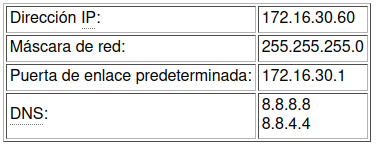
\includegraphics[scale=0.80]{eth-config.png}
        \caption{Datos a configurar en la interfaz eth de la MV}
    \end{figure}

    Cuando realices las capturas necesarias, y antes de proceder a ejecutar los comandos que se indican a continuación, deshaz los cambios que hayas hecho en la configuración de la interfaz de red Ethernet para asegurarte de que tienes conexión a Internet.

    \item Ahora, desde la línea de comandos ejecuta los siguientes comandos, haz una captura de su salida y comenta brevemente la salida obtenida:

    \begin{enumerate}
        \item ipconfig /all
        \item hostname
        \item nslookup <nombre\_dominio>
        \item ping <dirección\_ip>
        \item tracert <dirección\_ip>
    \end{enumerate}

    Asegúrate de que el nombre de dominio y las direcciones IP corresponden a sitios web públicos de Internet, y no a tu dispositivo local (es decir, no uses "localhost", 127.0.0.1 o similar) o a otros dispositivos de tu red local (no vale la dirección de tu router tipo 192.168.1.1 o similares), y de que la salida de los comandos es correcta.
\end{enumerate}

\textbf{Capturas}:

\begin{itemize}
    \item Ventana donde se modifica la configuración de red (se debe indicar textualmente cómo se accede a dicha ventana).
    \item Muestra de que la configuración de red se ha modificado.
    \item Ejecución de cada uno de los comandos y salida producida.
\end{itemize}

\subsubsection{Solución}

En este primer ejercicio vamos a modificar la configuración del adaptador Ethernet de nuestra máquina virtual con Windows 10, para a continuación ejecutar diferentes comandos relacionados con redes y mostrar sus salidas.

\begin{enumerate}
    \item Primero, vamos a cambiar la configuración del adaptador ethernet.

    Para acceder a la configuración, pulsamos en \textbf{Menu Inicio ---> Redes e Internet}. Se nos abrirá una ventana con diferentes configuraciones que podemos realizar, pero a nosotros no interesa la opción \textbf{Cambiar opciones de adaptador}, así que pulsamos aquí.

    Esto nos abrirá la venta de \textbf{Conexiones de red}, donde se nos mostrarán todos los adaptadores de red que tenemos configurados. En nuestro caso, solo tenemos el adaptador \textbf{Ethernet0}, así que hacemos doble-click sobre este adaptador, lo que nos abrirá una ventana con información sobre su estado. En esta ventana, en la parte inferior, pulsamos en el botón \textbf{Propiedades}, lo que nos abrirá otra ventana con las propiedades del adaptador.

    En esta nueva ventana, buscamos en la lista de elementos y seleccionamos \textbf{Protocolo de internet versión 4} y pulsamos en \textbf{Propiedades}. Se nos abrirá una ventana, la cual podemos ver en la siguiente captura, donde podremos cambiar la configuración IPv4 del adaptador.

    \begin{figure}[H]
        \centering
        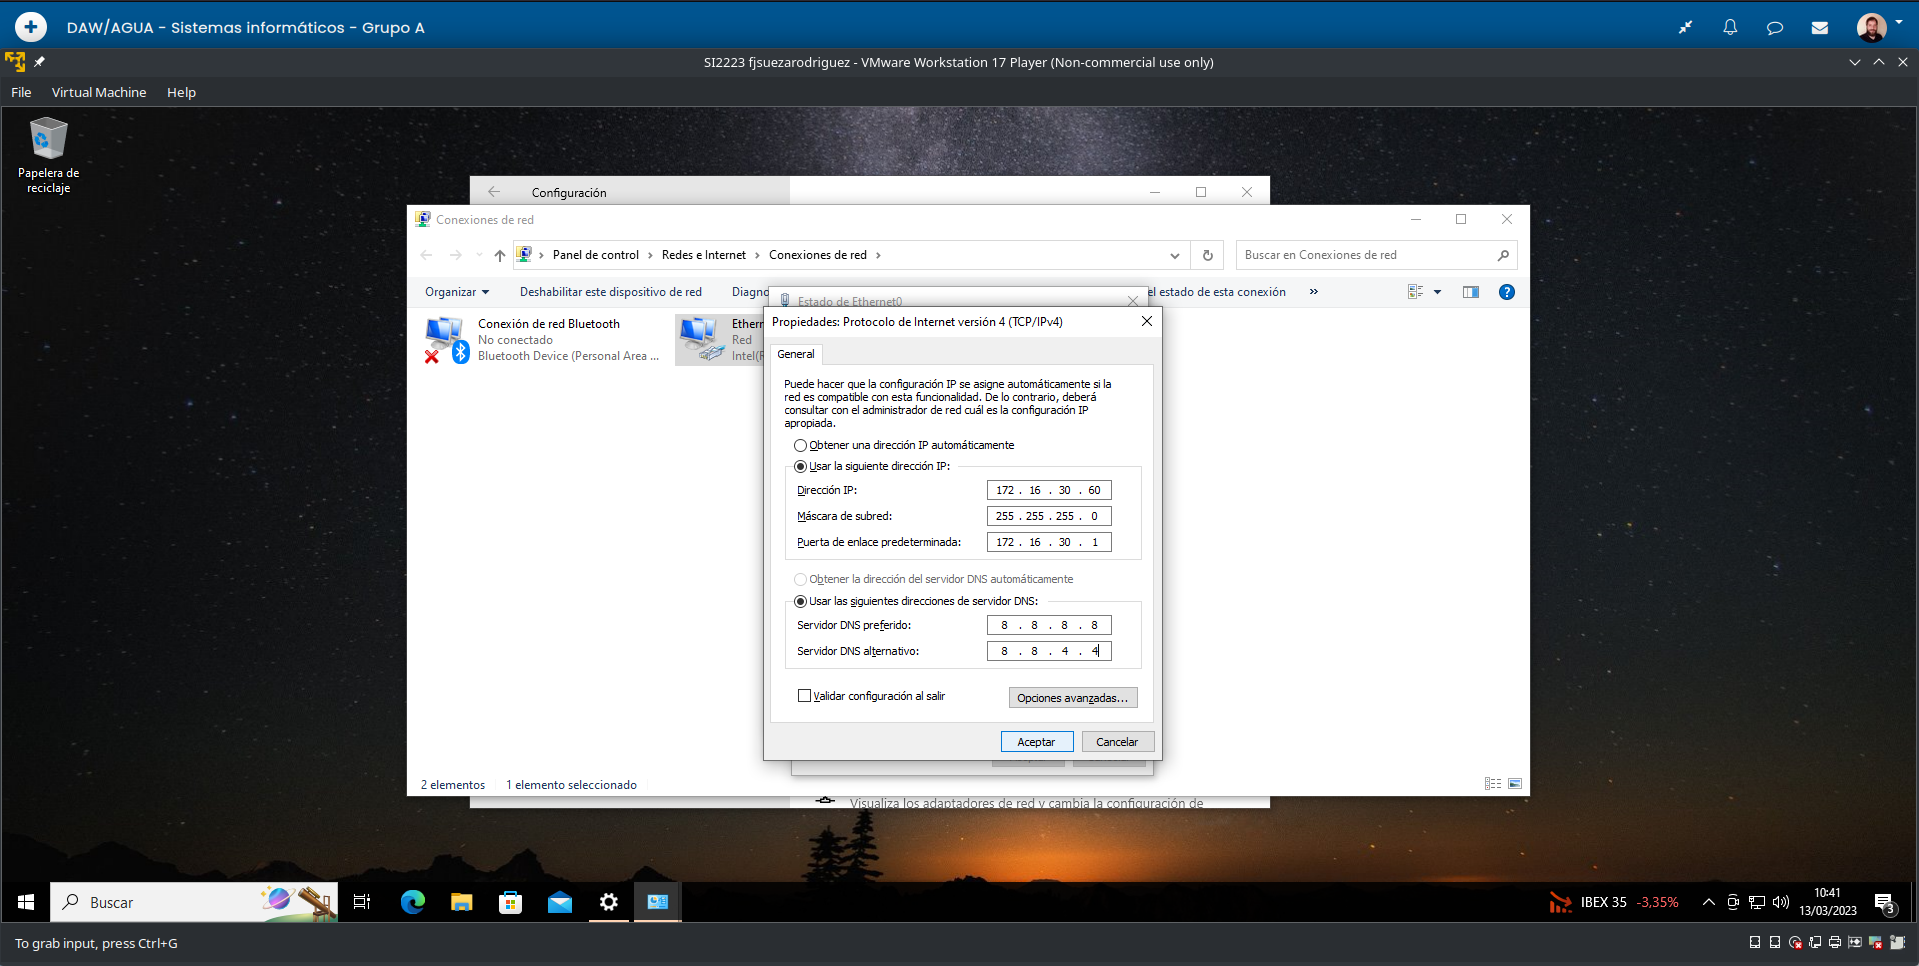
\includegraphics[scale=0.19]{eth0-config.png}
        \caption{Cambio de valores de la interfaz Ethernet0}
    \end{figure}

    Para comprobar que se ha realizado el cambio correctamente, volvemos a la venta de \textbf{Estado de Ethernet0} y pulsamos en \textbf{Detalles}, lo que nos mostrará toda la información de red, como se ve a continuación.

    \begin{figure}[H]
        \centering
        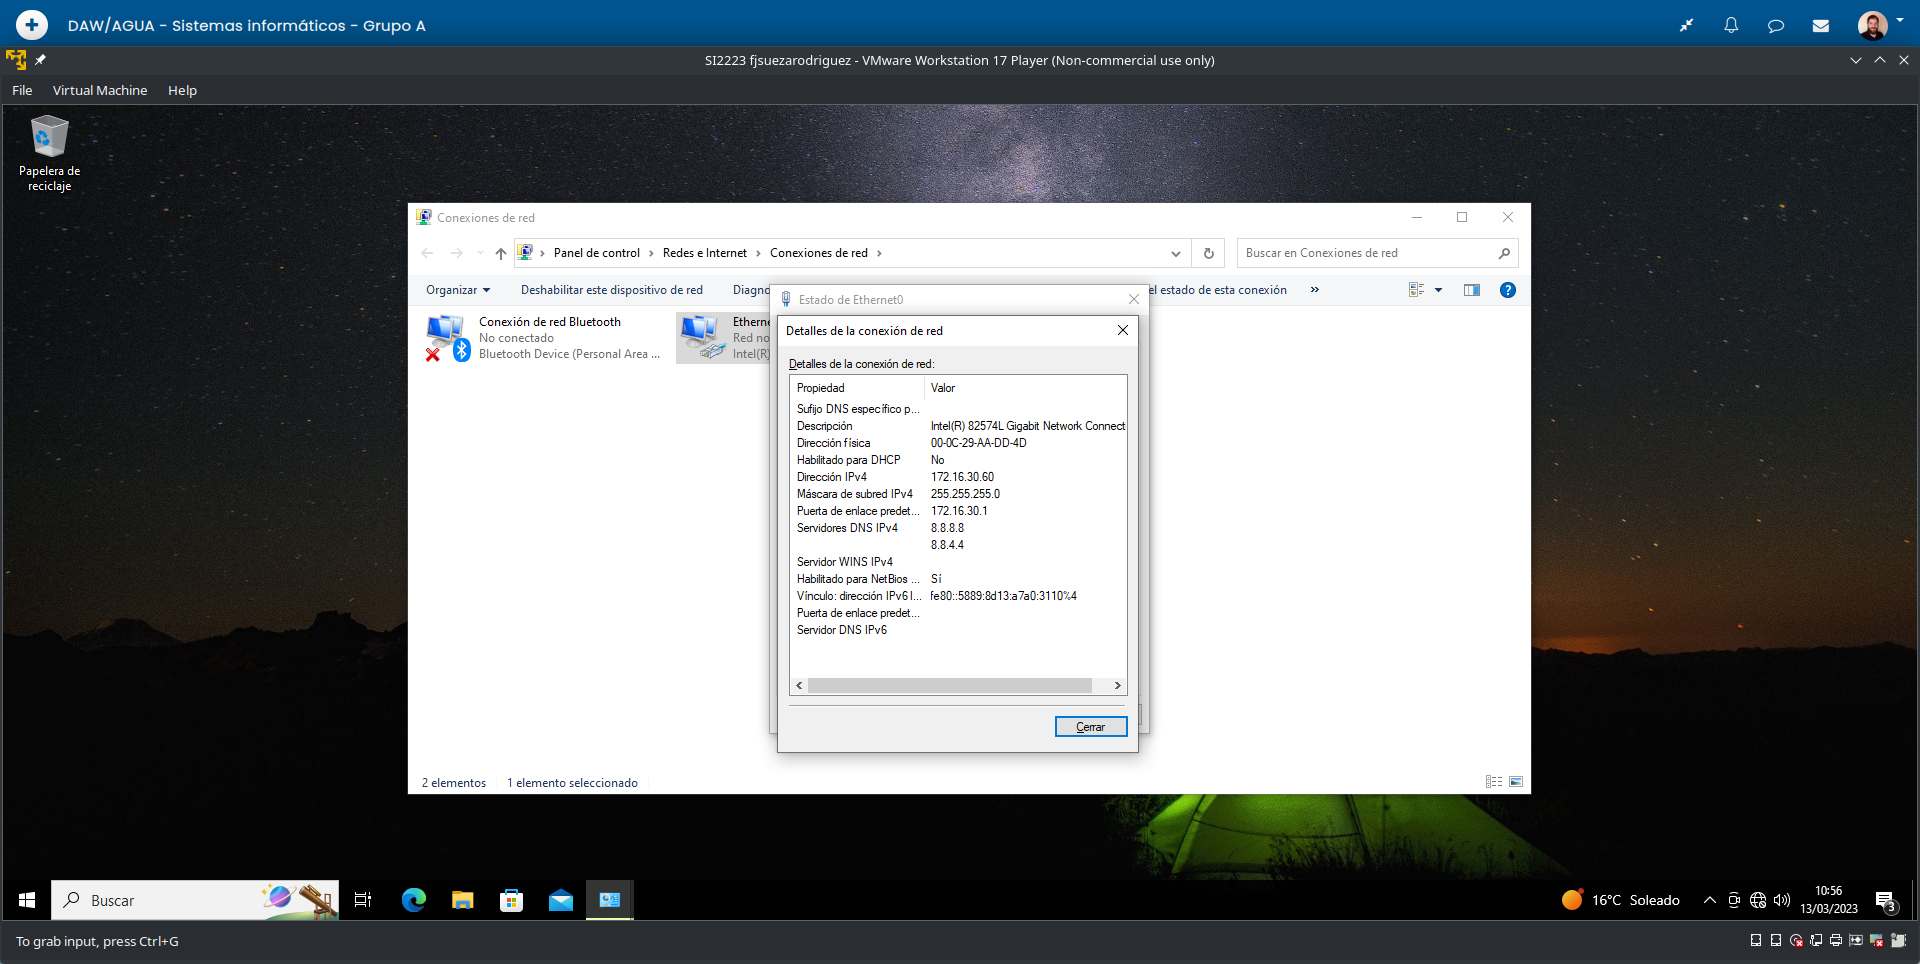
\includegraphics[scale=0.19]{eth0-config-2.png}
        \caption{Información de la interfaz Ethernet0 con los datos se han cambiado}
    \end{figure}

    \item A continuación, vamos a ejecutar una serie de \textbf{comandos de red} y a mostrar y comentar su salida.
    \begin{itemize}
        \item \textbf{ipconfig /all}: este comando nos ha mostrado la configuración de red. En concreto, la configuración \textbf{IP de Windows} y la de todas las interfaces de red que tenemos en el equipo, en nuestro caso, los de la interfaces \textbf{Ethernet0} y de la interfaz \textbf{Bluetooth}, esta última sin conexión a internet.

        \begin{figure}[H]
            \centering
            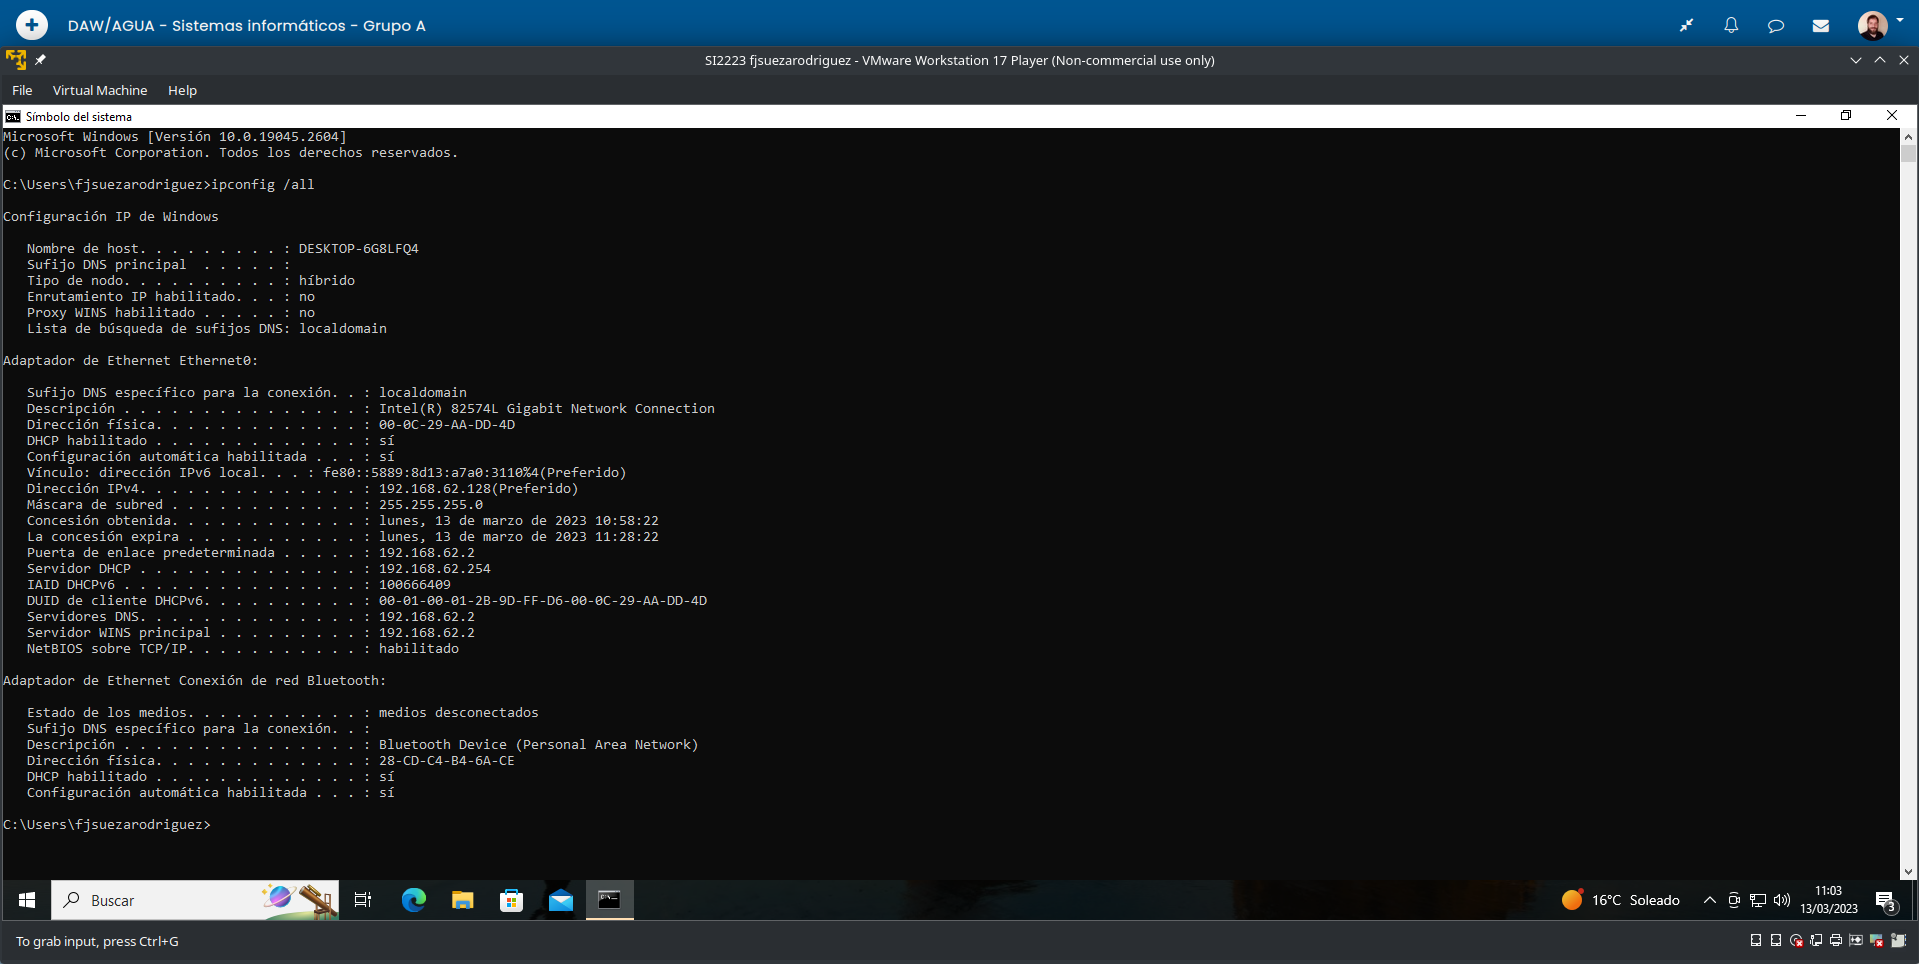
\includegraphics[scale=0.17]{commands-ipconfig.png}
            \caption{Salida del comando ipconfig}
        \end{figure}

        \item \textbf{hostname}: este comando simplemente nos muestra el nombre host de la máquina. En nuestro caso no hemos establecido ninguno por lo que tenemos el que establece por defecto Windows 10.

        \begin{figure}[H]
            \centering
            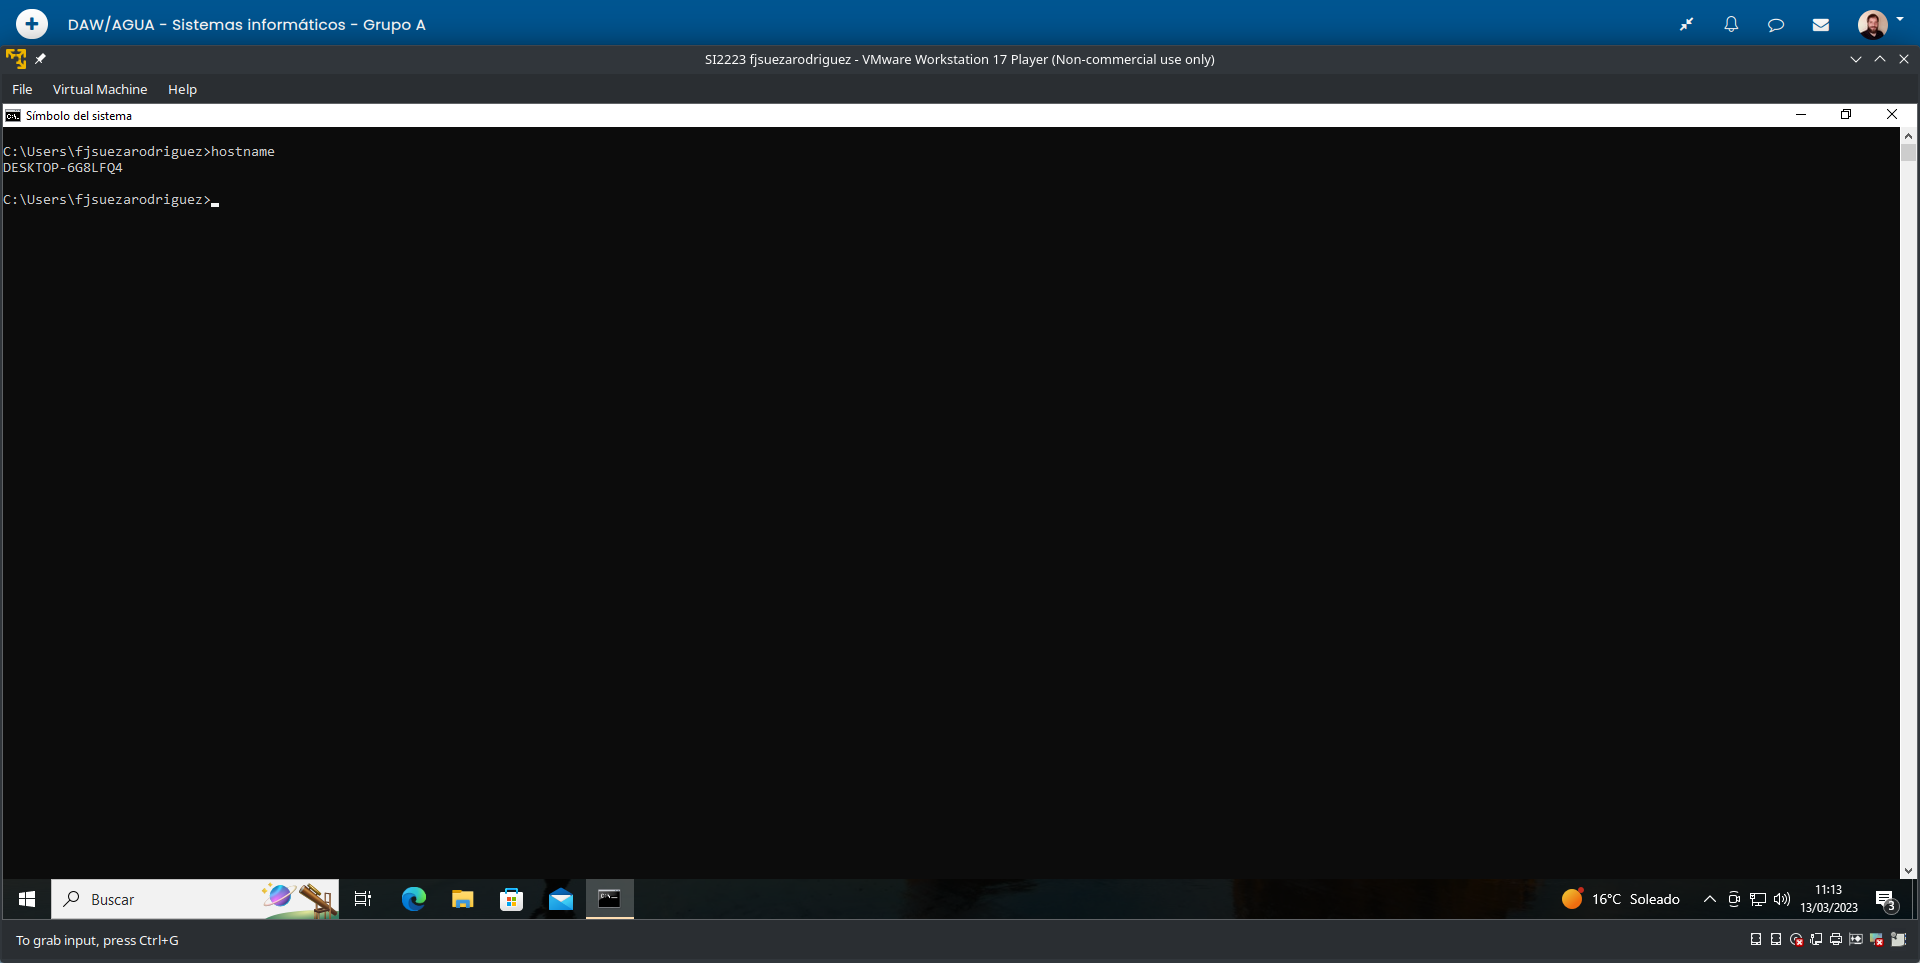
\includegraphics[scale=0.17]{commands-hostname.png}
            \caption{Salida del comando hostname}
        \end{figure}

        \item \textbf{nslookup}: este comando nos muestra información sobre DNS de un dominio o IP determinado. Nosotros hemos ejecutado el comando sobre \textbf{www.google.com}, mostrándonos en la salida información sobre la IP de este dominio.

        \begin{figure}[H]
            \centering
            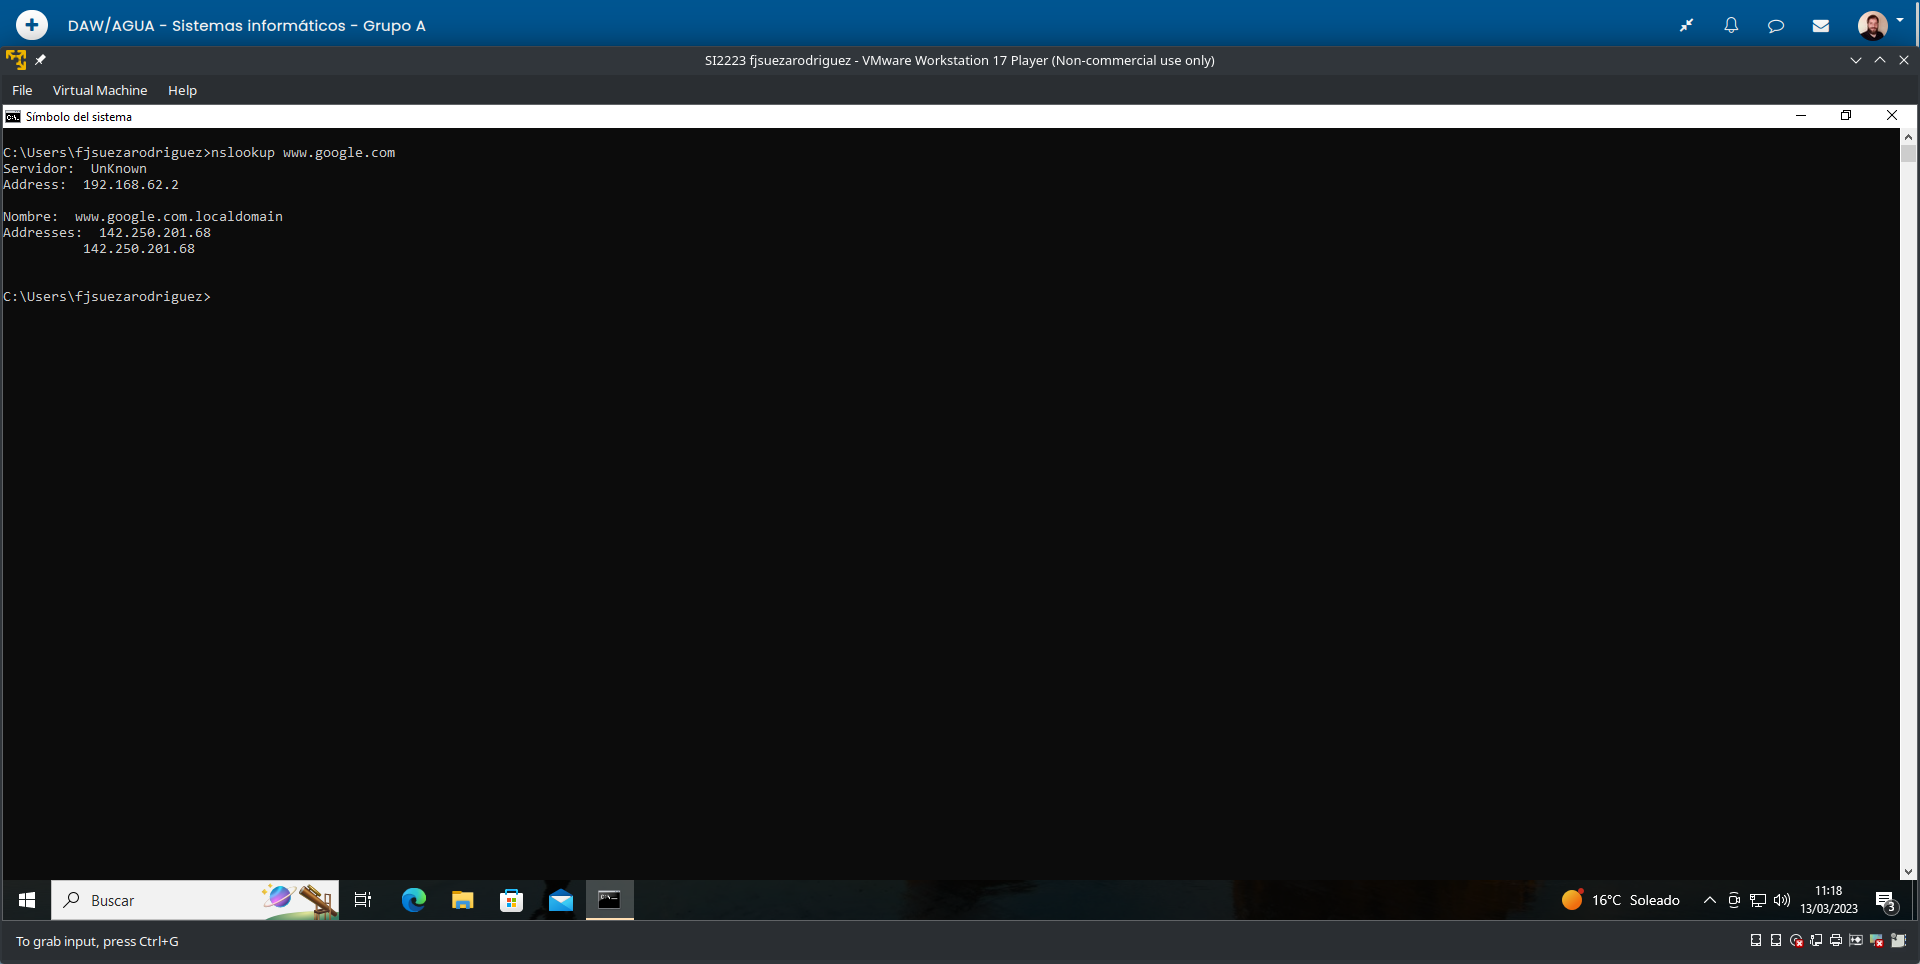
\includegraphics[scale=0.17]{commands-nslookup.png}
            \caption{Salida del comando nslookup}
        \end{figure}

        \item \textbf{ping}: este comando se usa para comprobar si hay conexión entre nuestro ordenador y una dirección de IP remota. Nosotros hemos realizado ping sobre \textbf{www.google.com} y como vemos se hay una conexión perfecta con esta dirección, con 0\% de paquetes perdidos y una \textbf{respuesta mínima de 25ms} y \textbf{máxima de 136ms}.

            \begin{figure}[H]
            \centering
            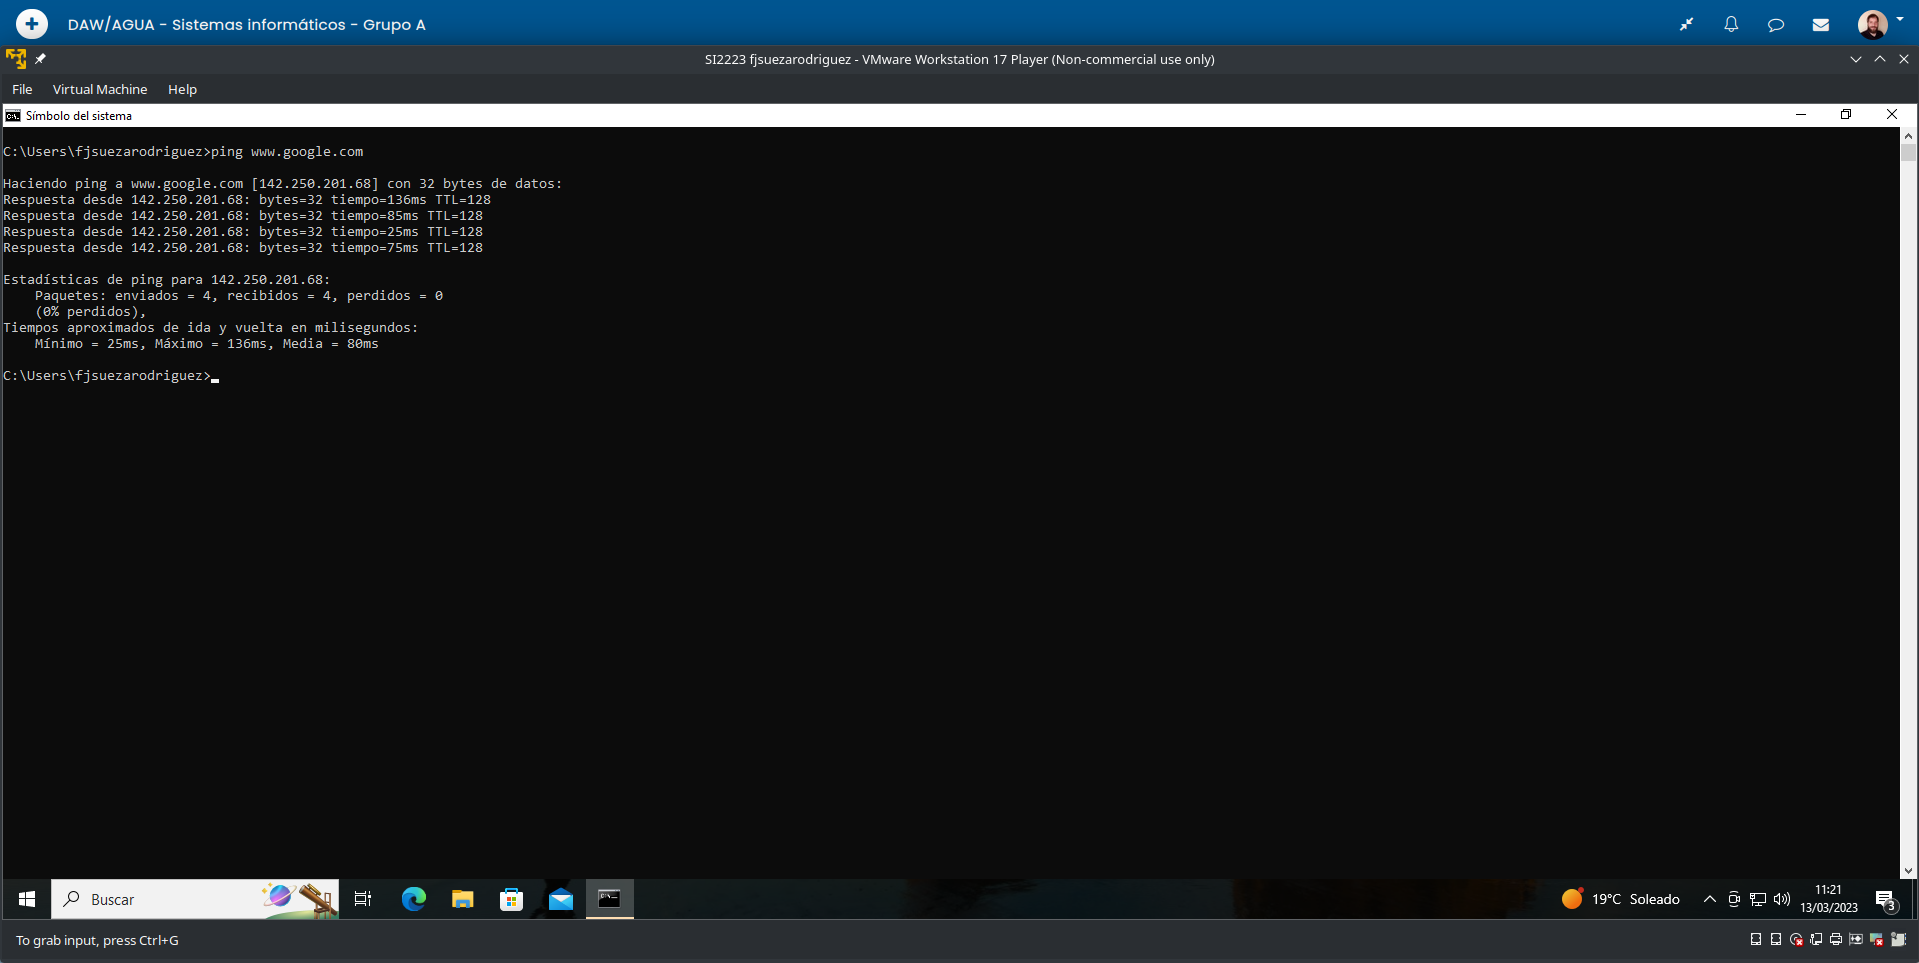
\includegraphics[scale=0.17]{commands-ping.png}
            \caption{Salida del comando ping}
        \end{figure}

        \item \textbf{tracert}: esta utilidad nos muestra todos los saltos que hay entre nuestro ordenador y una dirección ip determinada. En nuestro caso, hemos vuelto a ejecutarla sobre \textbf{wwww.google.com}. En nuestro caso como vemos hay \textbf{9 saltos} entre nuestra dirección y la de google, incluyendo nuestro router (192.168.1.1).

        \begin{figure}[H]
            \centering
            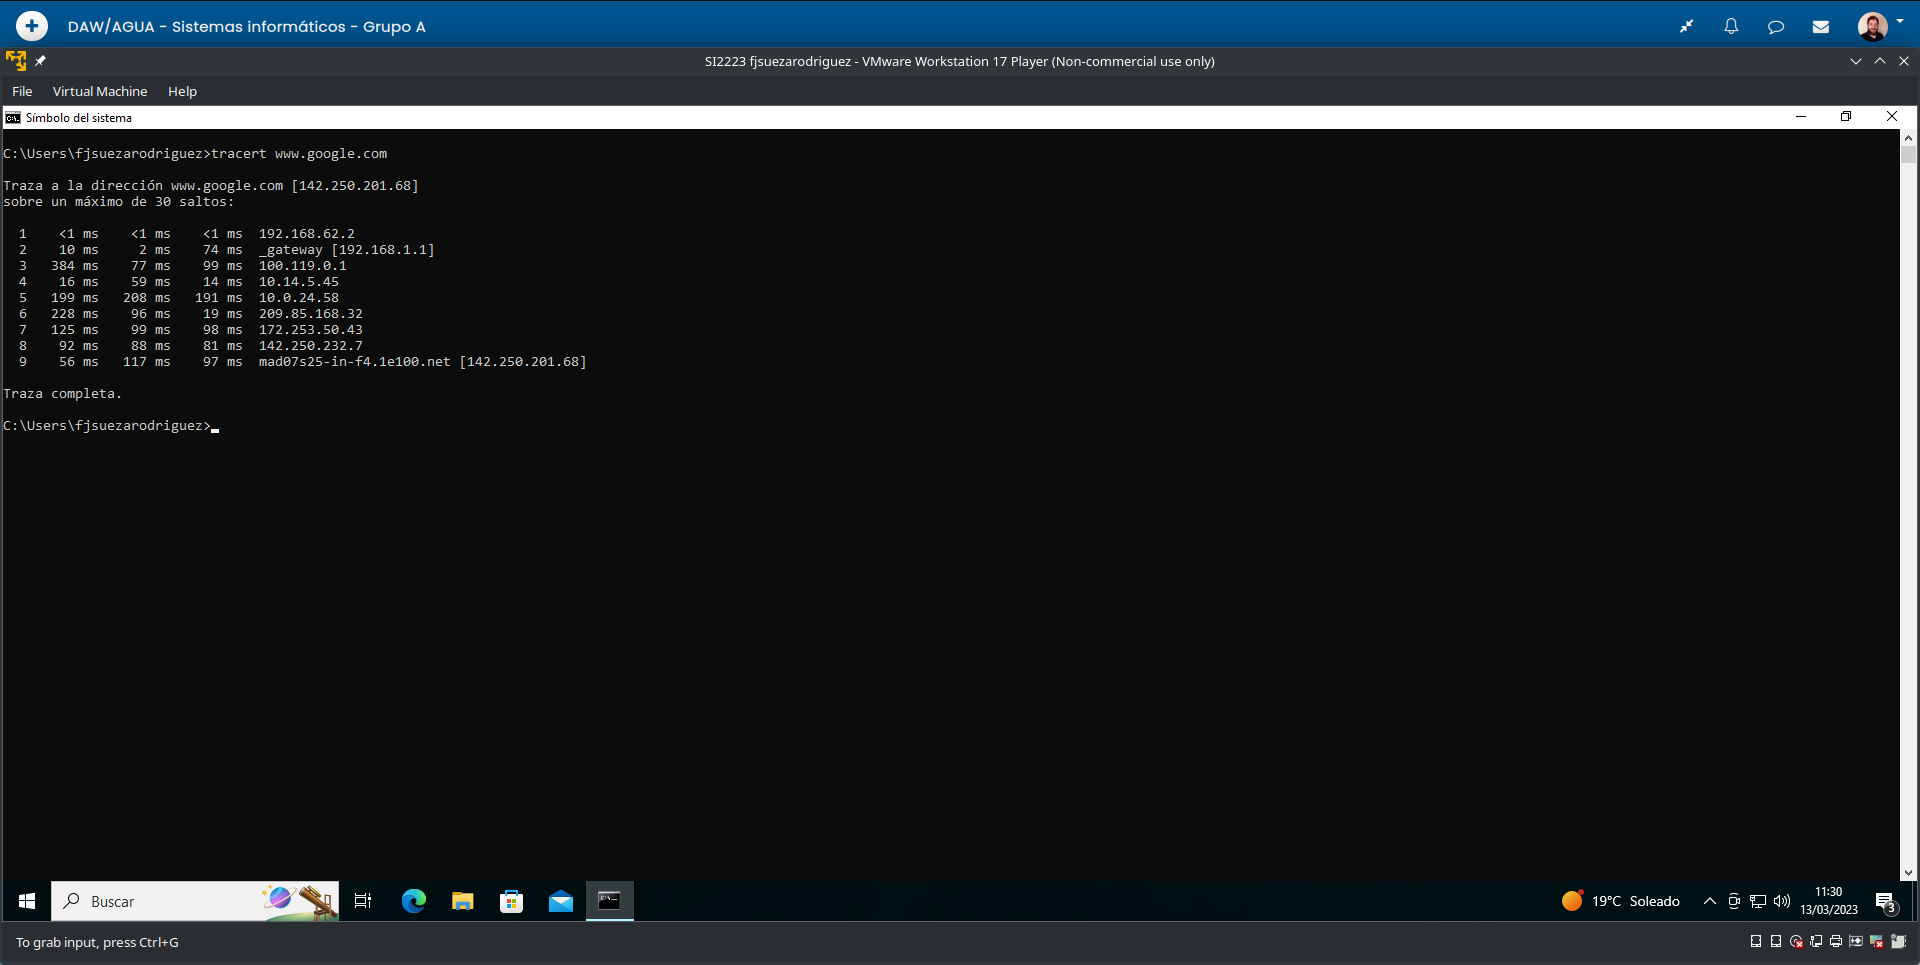
\includegraphics[scale=0.17]{commands-tracert.png}
            \caption{Salida del comando tracert}
        \end{figure}
    \end{itemize}
\end{enumerate}

\subsection{Actividad 2: Comunicar MV y Máquina Anfitriona en Red y Compartir una Carpeta}

\subsubsection{Enunciado}
Para esta actividad debes configurar la MV para que máquina anfitriona y máquina virtual puedan comunicarse a través de un entorno de red local. Puedes hacerlo de diversas maneras, las cuales serán más o menos adecuadas dependiendo de tu entorno de red. Recomendamos una de estas dos opciones:

\begin{itemize}
    \item \textbf{Opción 1}: Estableciendo el adaptador de red de la MV en modo ``puente''. En este caso el software de virtualización simulará que la MV esté conectada directamente al mismo aparato que tu máquina anfitriona. Por ejemplo, si tienes un router casero, será como si la MV estuviese conectada directamente al router con una conexión cableada y pertenecerá a su subred LAN igual que el equipo anfitrión.

    \item \textbf{Opción 2}: Habilitar un segundo adaptador de red en la MV y configurarlo en modo ``sólo-anfitrión''. Esto simula una segunda tarjeta de red en la MV, la cual estaría conectada directamente a otra tarjeta de red en la máquina anfitriona. Para esta conexión la máquina anfitriona utiliza un adaptador de red virtual que se crea durante la instalación del software de virtualización. En el caso de VirtualBox este adaptador se llama ``VirtualBox Host-Only Network'' y por defecto tiene la IP 192.168.56.1/24, por lo que en la máquina virtual tendrías que asegurarte de que el segundo adaptador de red que has añadido tiene una IP que pertenezca a la misma subred. El motivo de tener dos adaptadores de red en este caso es que el primero, configurado en modo NAT (el modo por defecto), permite a la MV tener conexión externa con Internet pero no con el anfitrión, mientras que el segundo, en modo sólo-anfitrión, permite la comunicación entre anfitrión y MV pero no con Internet.
\end{itemize}

Cuando hayas configurado la MV comprueba que existe comunicación entre ambas máquinas realizando dos ``ping'': uno de la MV a la máquina anfitriona y otro al contrario. Es posible que para que funcione el ``ping'' debas activar en las máquinas la opción de ``activar el uso compartido de archivos e impresoras'', o bien una regla en el firewall de Windows que permita el tráfico de ``solicitud de eco ICMP''.

Cuando compruebes que existe comunicación a través de la red entre ambas máquinas, crea una carpeta en la máquina virtual y compártela. Deberás acceder a esta carpeta desde la máquina anfitriona a través de la red y crear un documento en su interior con algún texto de ejemplo. Esta acción de compartir la carpeta no se puede realizar utilizando las herramientas que proveen los programas de virtualización para ello, debe hacerse tal como se haría si se tuviesen dos equipos conectados dentro de una red local.

\textbf{Capturas}:

\begin{itemize}
    \item Configuración del adaptador de red de la máquina virtual en el software de virtualización.
    \item Configuración IP del adaptador de la máquina real que se vaya a usar para la comunicación.
    \item Configuración IP del adaptador de la máquina virtual que se vaya a usar para la comunicación.
    \item Ping máquina virtual > máquina anfitriona.
    \item Ping máquina anfitriona > máquina virtual.
    \item Compartición de la carpeta creada en la MV.
    \item Acceso desde la máquina anfitriona a la carpeta compartida en la MV.
    \item Creación de un documento de texto dentro de la carpeta compartida desde la máquina anfitriona.
\end{itemize}

\subsubsection{Solución}
En este ejercicio vamos a conectar mediante red la máquina anfitriona y la máquina visitante. Nosotros, hemos elegido la \textbf{opción 1} para conectar ambas máquinas, ya nos ha parecido más simple y ciertamente, ha sido bastante rápida y efectiva. A continuación detallamos los pasos que hemos llevado a cabo.

\begin{enumerate}
    \item En primer lugar hemos cambiado la configuración del adaptador ethernet de VMWare, estableciendo el adaptador de red en modo \textbf{bridge} y marcando la casilla \textbf{Replicate physical network connection state}, como se puede ver en la siguiente captura.

    \begin{figure}[H]
        \centering
        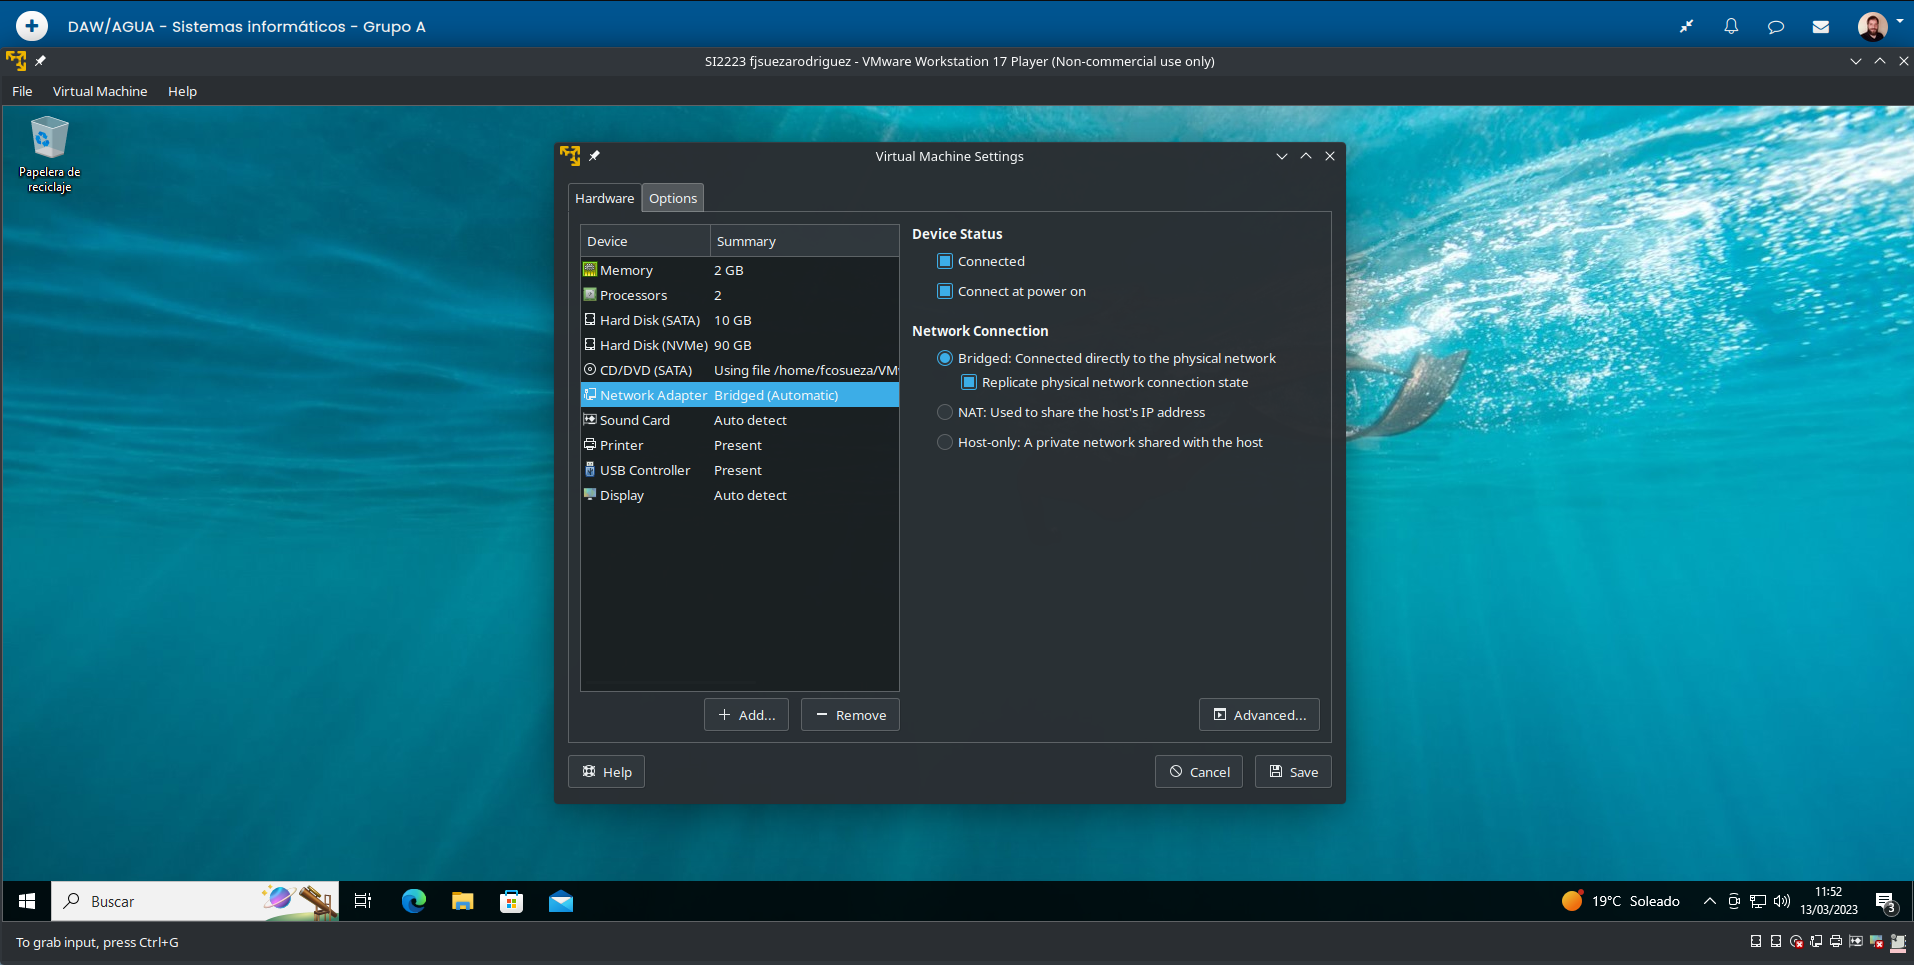
\includegraphics[scale=0.18]{connect-1.png}
        \caption{Estableciendo el adaptador de red de VMWare en modo bridge}
    \end{figure}

    \item En este paso, \textbf{no hemos tenido} que hacer ninguna \textbf{configuración de los adaptadores} del red ni del sistema host ni del guest, ya que al establecer el adaptador de VMWare en modo bridge el \textbf{sistema invitado se conecta} a la red como \textbf{una máquina más de la red}. Aun así, aquí se muestran 2 capturas con la configuración que tiene cada una de las máquinas.

    \begin{figure}[H]
        \centering
        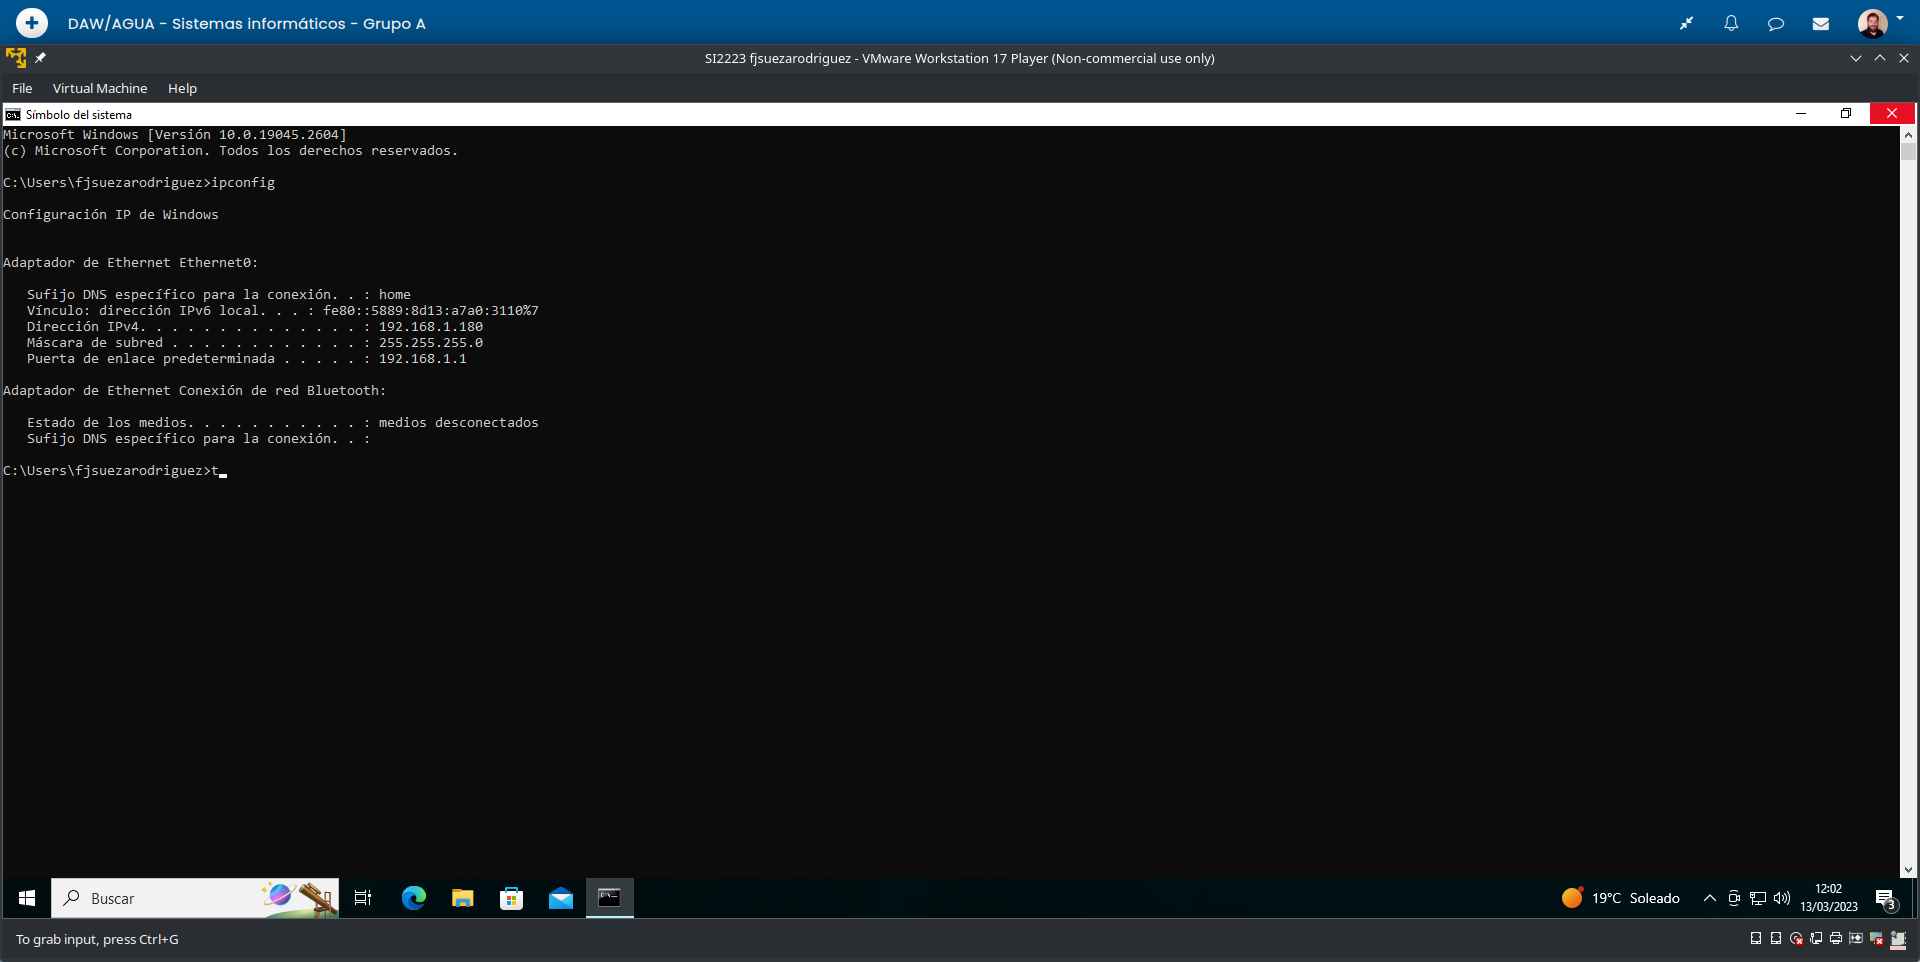
\includegraphics[scale=0.18]{connect-2.png}
        \caption{Configuración de la interfaz de red del invitado}
    \end{figure}

    \begin{figure}[H]
        \centering
        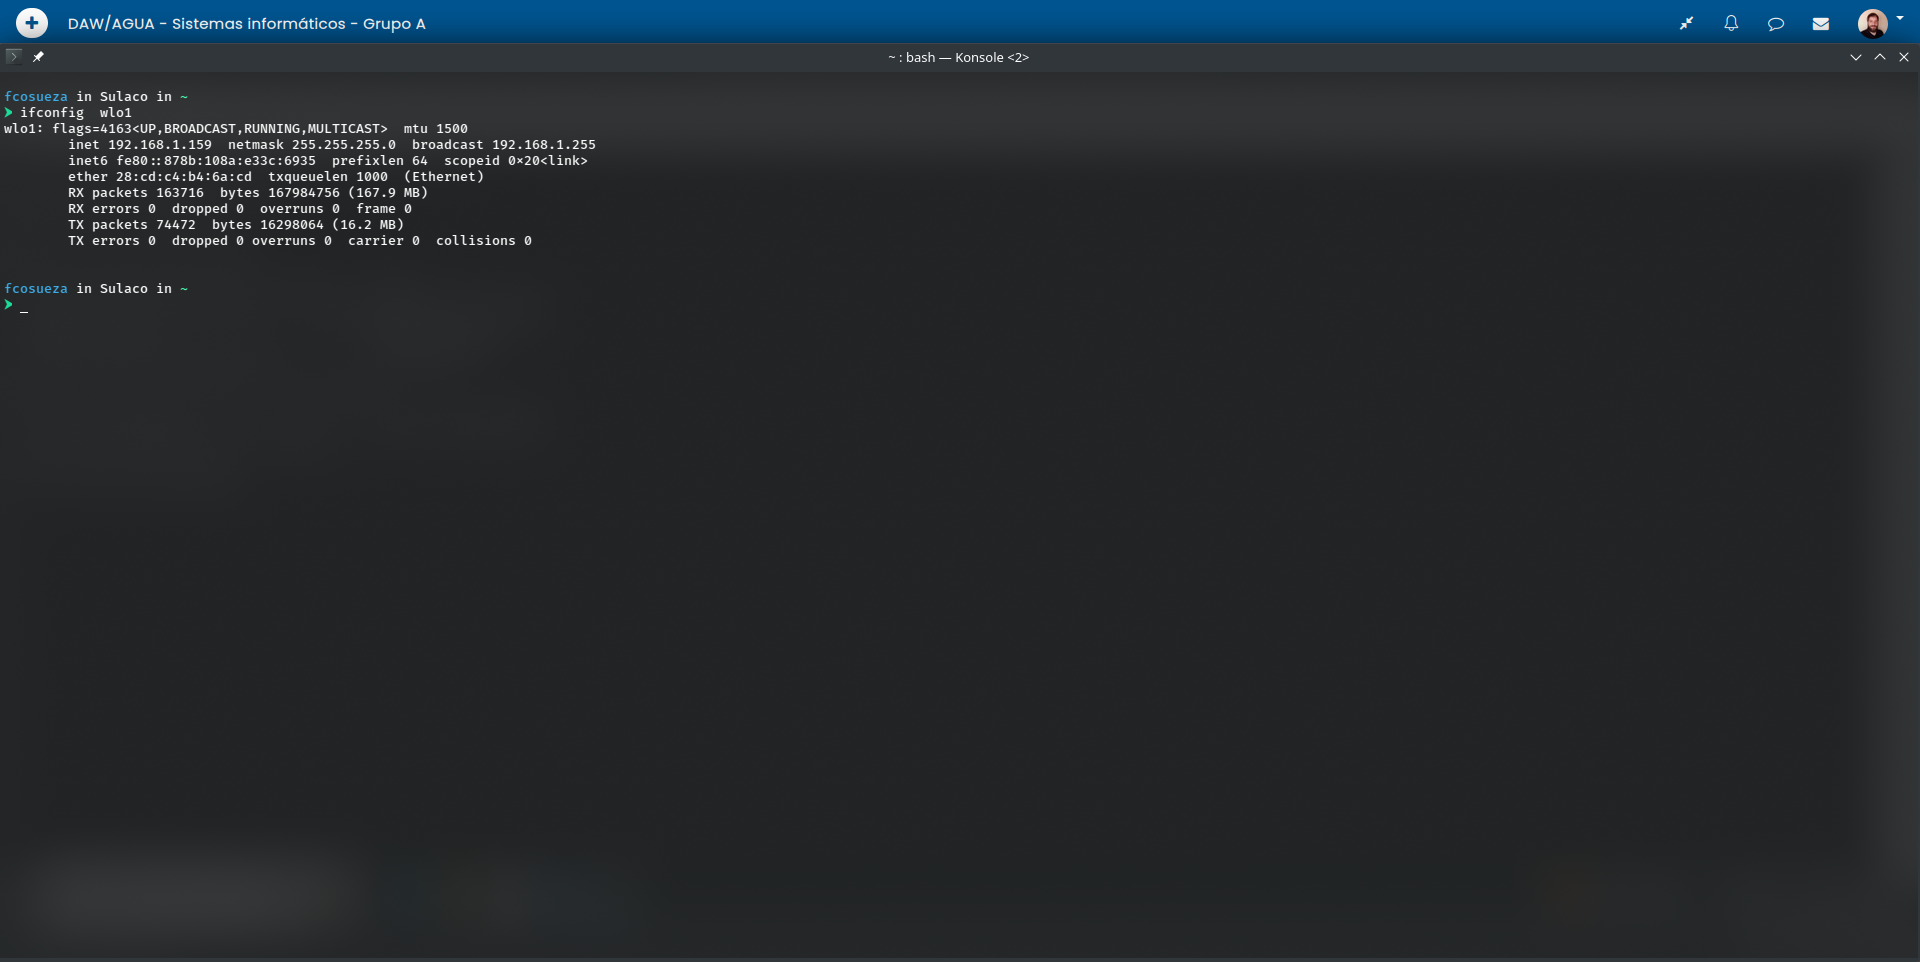
\includegraphics[scale=0.18]{connect-3.png}
        \caption{Configuración de la interfaz de red del anfitrión}
    \end{figure}

    \item Para comprobar que se ha establecido la conexión correctamente, hemos usado el comando \textbf{ping} entre las dos máquinas. Cabe destacar que para que funcione el comando, hemos tenido que activar la opción \textbf{Activar uso compartido de archivos e impresoras} en el sistema invitado. Una vez hecho esto, las máquinas se han reconocido correctamente, como vemos en las siguientes capturas.

    \begin{figure}[H]
        \centering
        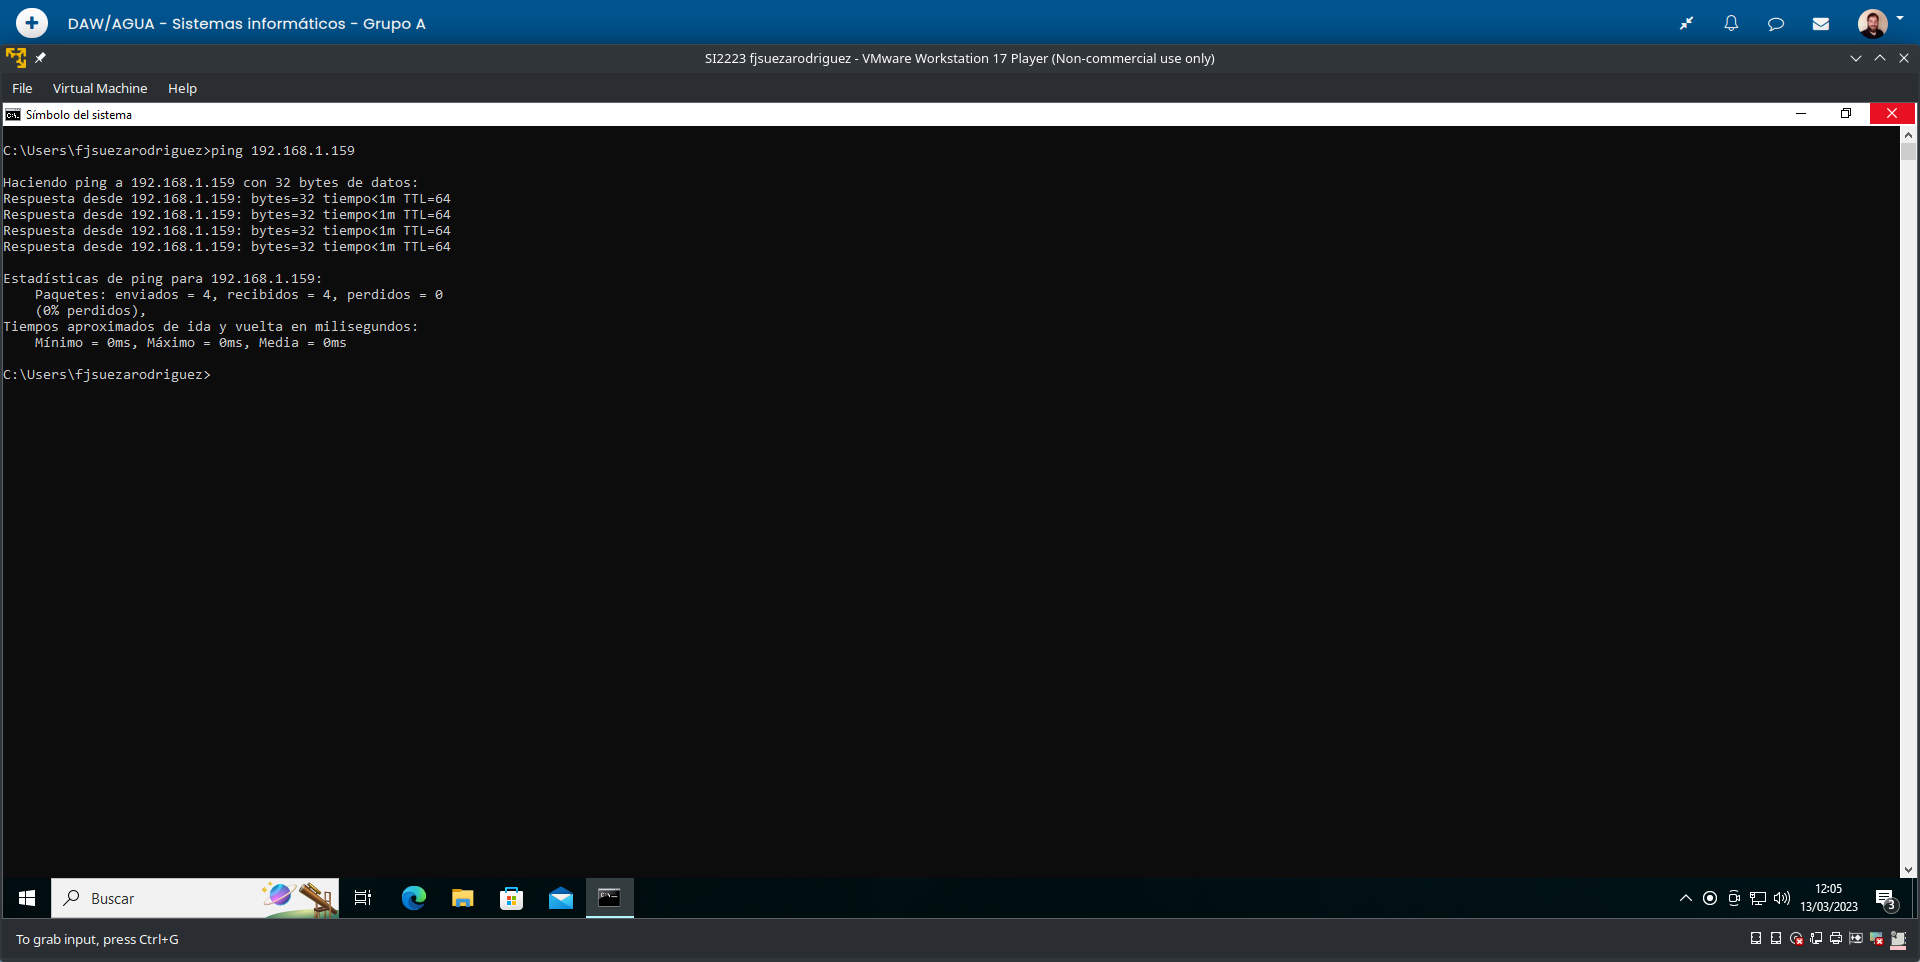
\includegraphics[scale=0.18]{connect-4.png}
        \caption{Ping desde el sistema invitado al anfitrión}
    \end{figure}

    \begin{figure}[H]
        \centering
        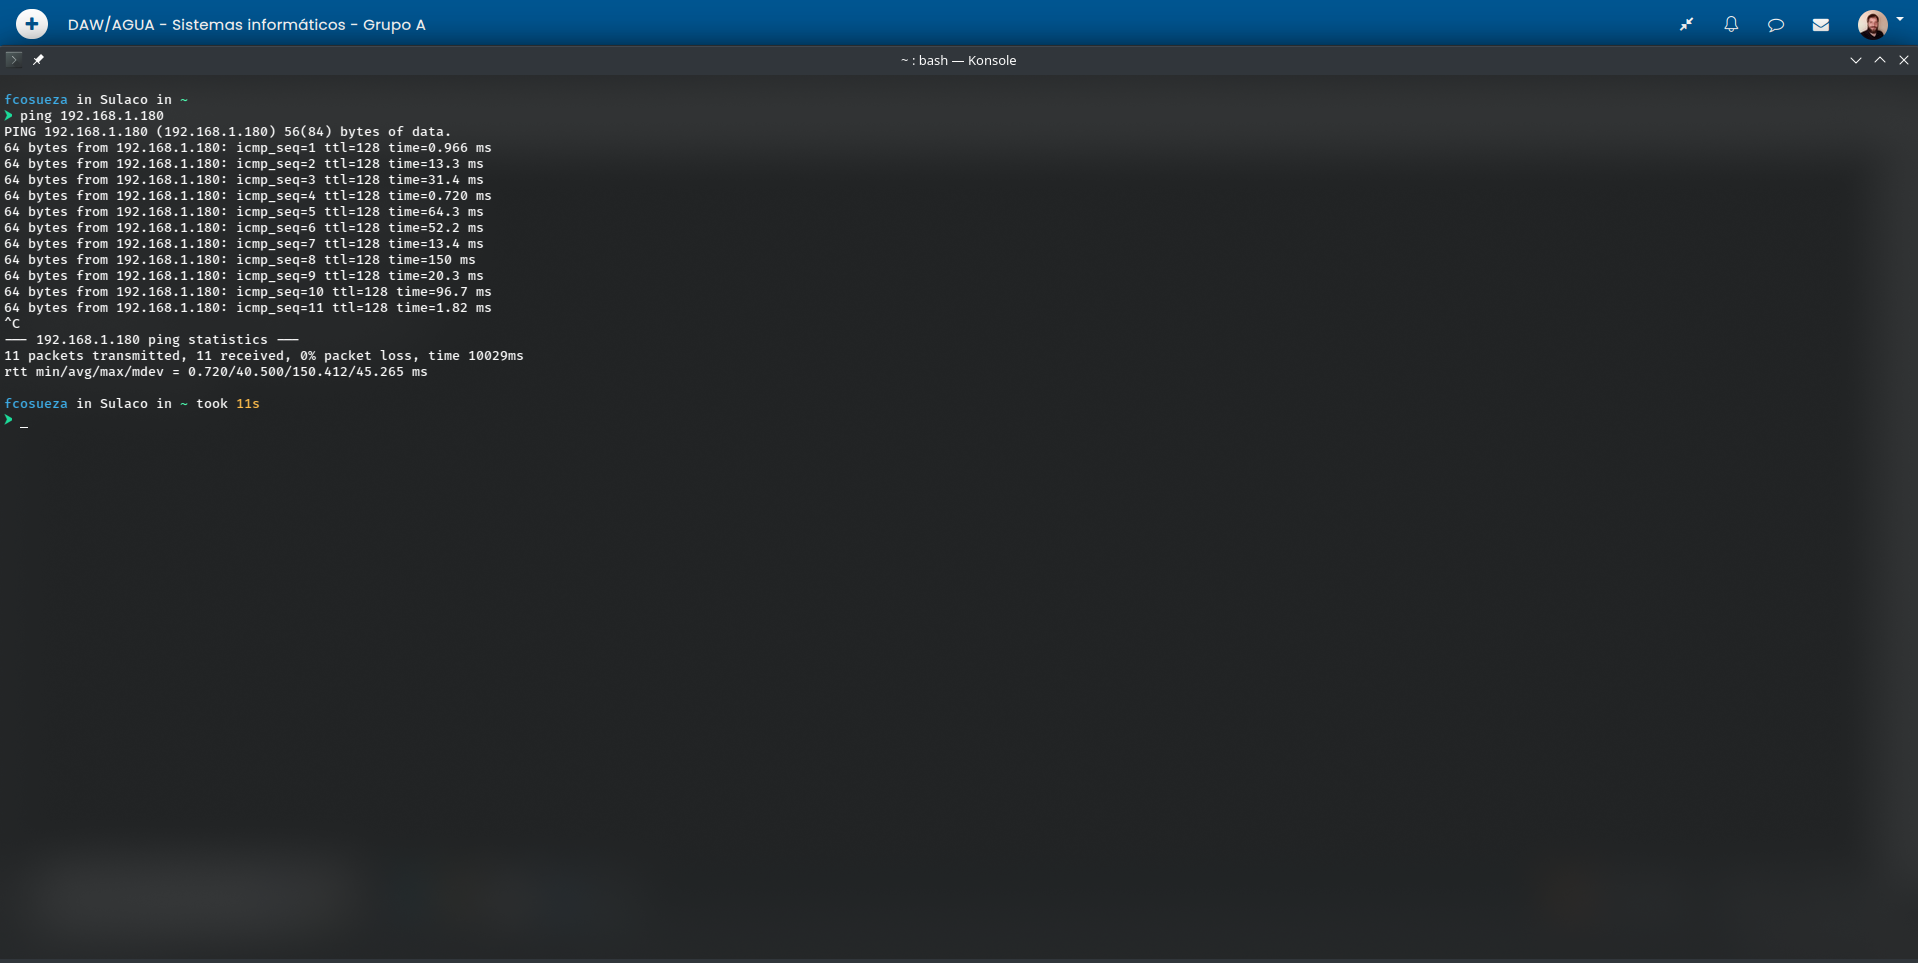
\includegraphics[scale=0.18]{connect-5.png}
        \caption{Ping desde el sistema anfitrión al invitado}
    \end{figure}

    \item Por último, hemos creado una carpeta compartida, que en un alarde de originalidad hemos llamado \textbf{Compartida}, en Windows 10 (sistema invitado). Pulsando en el botón derecho sobre la carpeta hemos accedido a \textbf{Propiedades}, y en la ventana que se nos abre a la pestaña \textbf{Compartir}. Hemos configurado la carpeta para que se comparta mediante la red, añadiendo permisos de escritura y lectura a todos los usuarios, entre otras cosas.

    En sistema anfitrión, una \textbf{Kubuntu 22.04}, hemos tenido que instalar \textbf{samba}, para poder acceder a estas carpeta, aunque aquí no vamos a entrar en detalles. Pero como podemos ver en la siguiente captura, ya podemos visualizar y acceder a la carpeta compartida desde Windows 10.

    \begin{figure}[H]
        \centering
        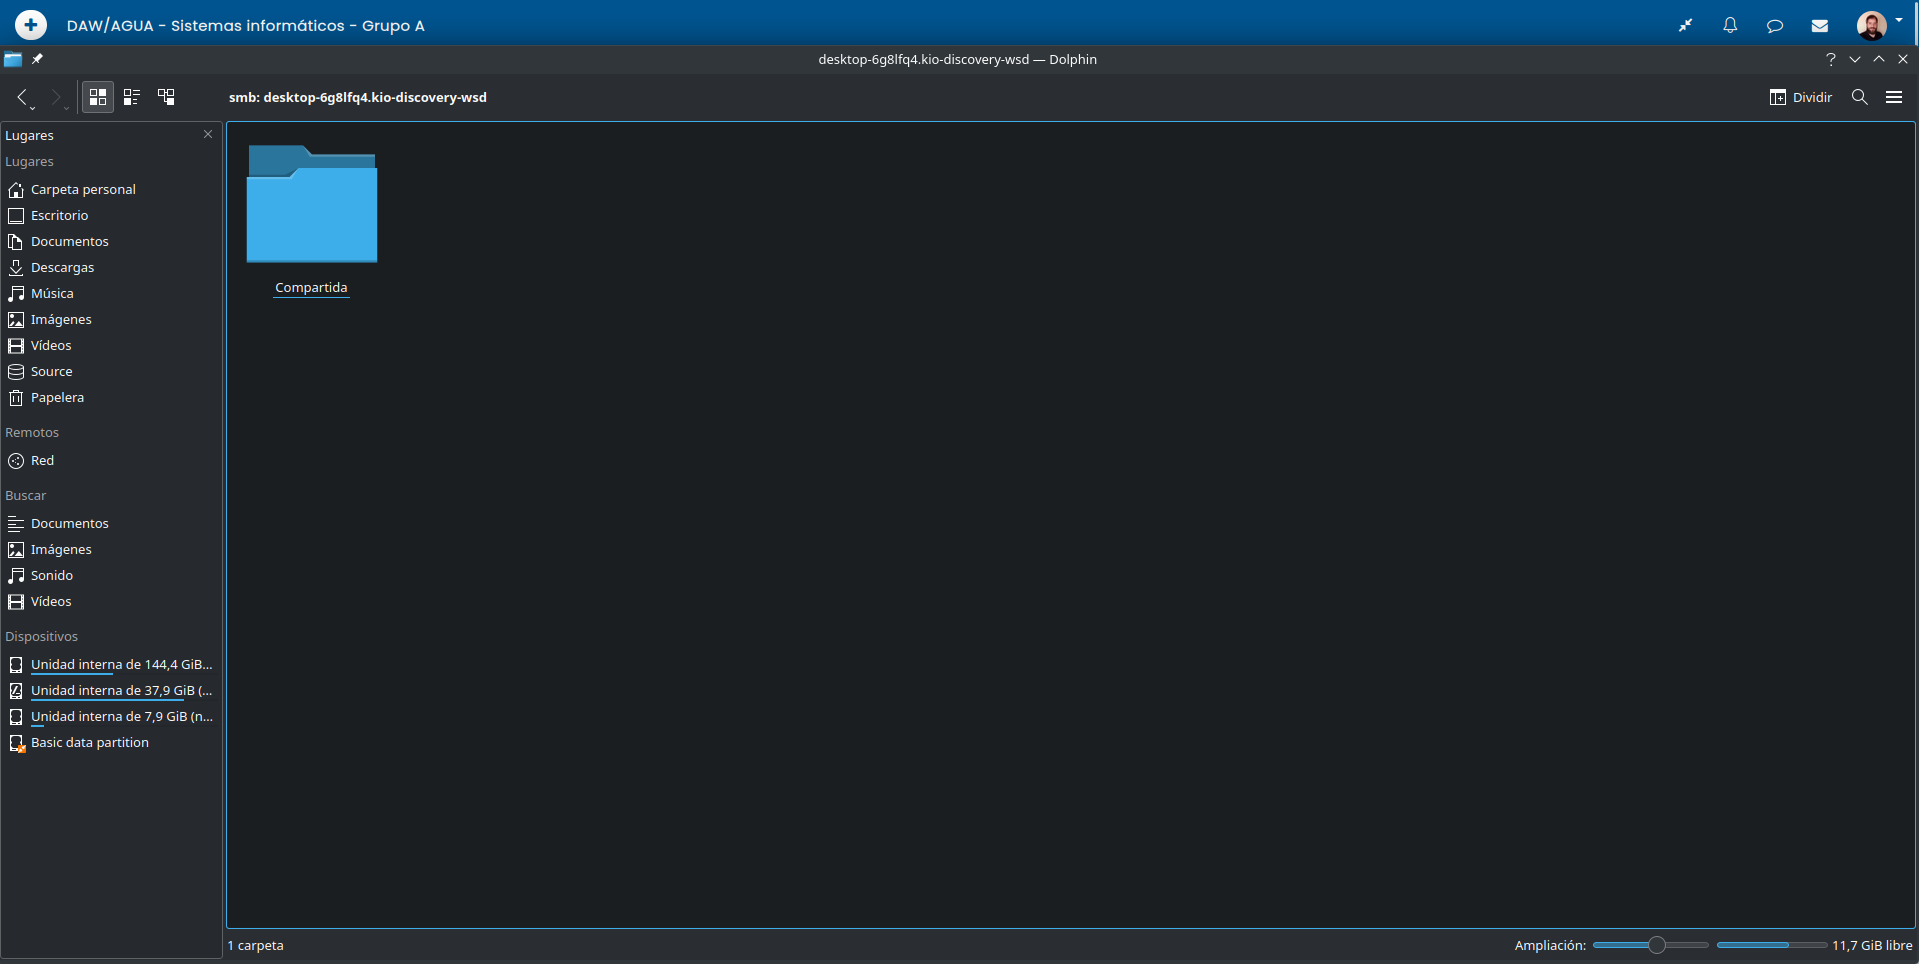
\includegraphics[scale=0.18]{connect-6.png}
        \caption{Carpeta compartida visible desde el anfitrión}
    \end{figure}

    A continuación hemos creado un archivo de texto desde el anfitrión y lo hemos abierto desde el invitado, para comprobar que se había creado correctamente.

    \begin{figure}[H]
        \centering
        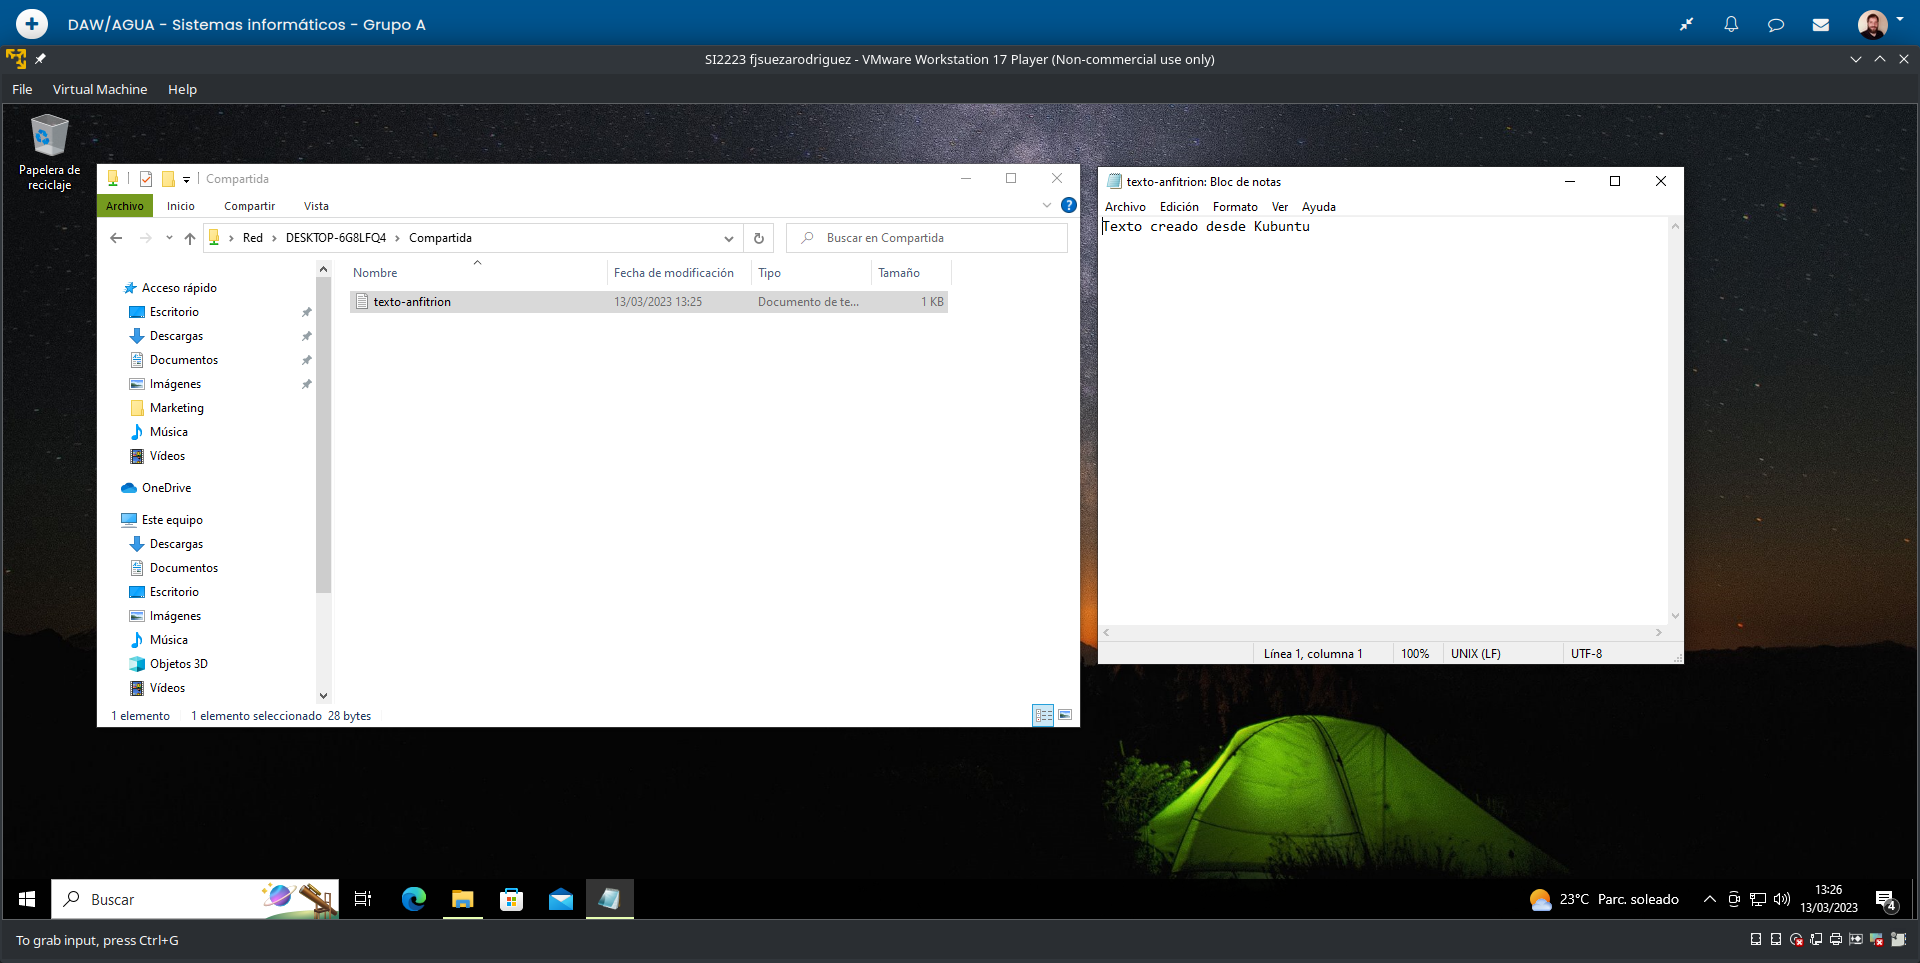
\includegraphics[scale=0.18]{connect-7.png}
        \caption{Archivo creado desde el sistema anfitrión abierto en el invitado}
    \end{figure}
\end{enumerate}

\subsection{Actividad 3: Establece un Servidor FTP Básico en Windows 10}

\subsubsection{Enunciado}
Instala y configura en la MV un servidor FTP con el servicio de FTP que suministra Windows, con autenticación básica y requiriendo TLS/SSL (para ello se puede utilizar un certificado autofirmado). El nombre del sitio FTP será ``SI\_<inicial de tu nombre y primer apellido>''. Por ejemplo, para un alumno llamado Pablo Rodríguez Campos, el nombre de su sitio FTP será ``SI\_prodriguez''. Si tienes problemas para conseguir que funcione la conexión mediante TLS/SSL utiliza el foro de la unidad para consultarlo.

El acceso a dicho servidor lo realizarás desde la máquina anfitriona utilizando un cliente FTP como Filezilla. Una vez conectado al servidor realiza dos transferencias de ficheros: una descarga (MV > anfitrión) y una subida (anfitrión > MV).

Recuerda, el acceso será desde la máquina anfitriona (cliente FTP Filezilla) a la MV (servidor FTP incluido en Windows 10).

\textbf{Capturas}:

\begin{itemize}
    \item Creación y asignación de permisos a la carpeta usada para el directorio raíz del FTP.
    \item Activación de las características de Windows necesarias para el servicio FTP y su configuración.
    \item Creación del sitio FTP incluyendo: Nombre del sitio FTP y ruta de acceso física; Dirección IP de acceso, requerimiento de SSL y certificado; Tipo de autenticación, autorización de usuarios y permisos.
    \item Conexión del cliente FTP con el servidor. Se debe mostrar que esta conexión es segura mediante TLS/SSL.
    \item Descarga y subida de un fichero. Se debe ver en la consola de Filezilla que las transferencias han sido correctas.
\end{itemize}

\subsubsection{Solución}

En este ejercicio vamos a crear un servidor FTP en la máquina invitada con Windows 10 y posteriormente acceder a este desde la máquina anfitriona usando el cliente Filezilla. Para comprobar que el servidor funciona correctamente, haremos un par de transferencias de archivos.

\begin{enumerate}
    \item En primer lugar hemos creado la carpeta que será la raíz del servidor FTP. La carpeta creada se llama \textbf{SI\_fjsueza} y la hemos creado en el \textbf{Escritorio} de Windows. No ha sido necesario añadir permisos extra a dicha carpeta ya que vamos a usar el usuario que creamos al principio, \textbf{fjsuezarodriguez}, para acceder al servidor FTP, el cual ya tiene todos los permisos sobre dicha carpeta.

    \begin{figure}[H]
        \centering
        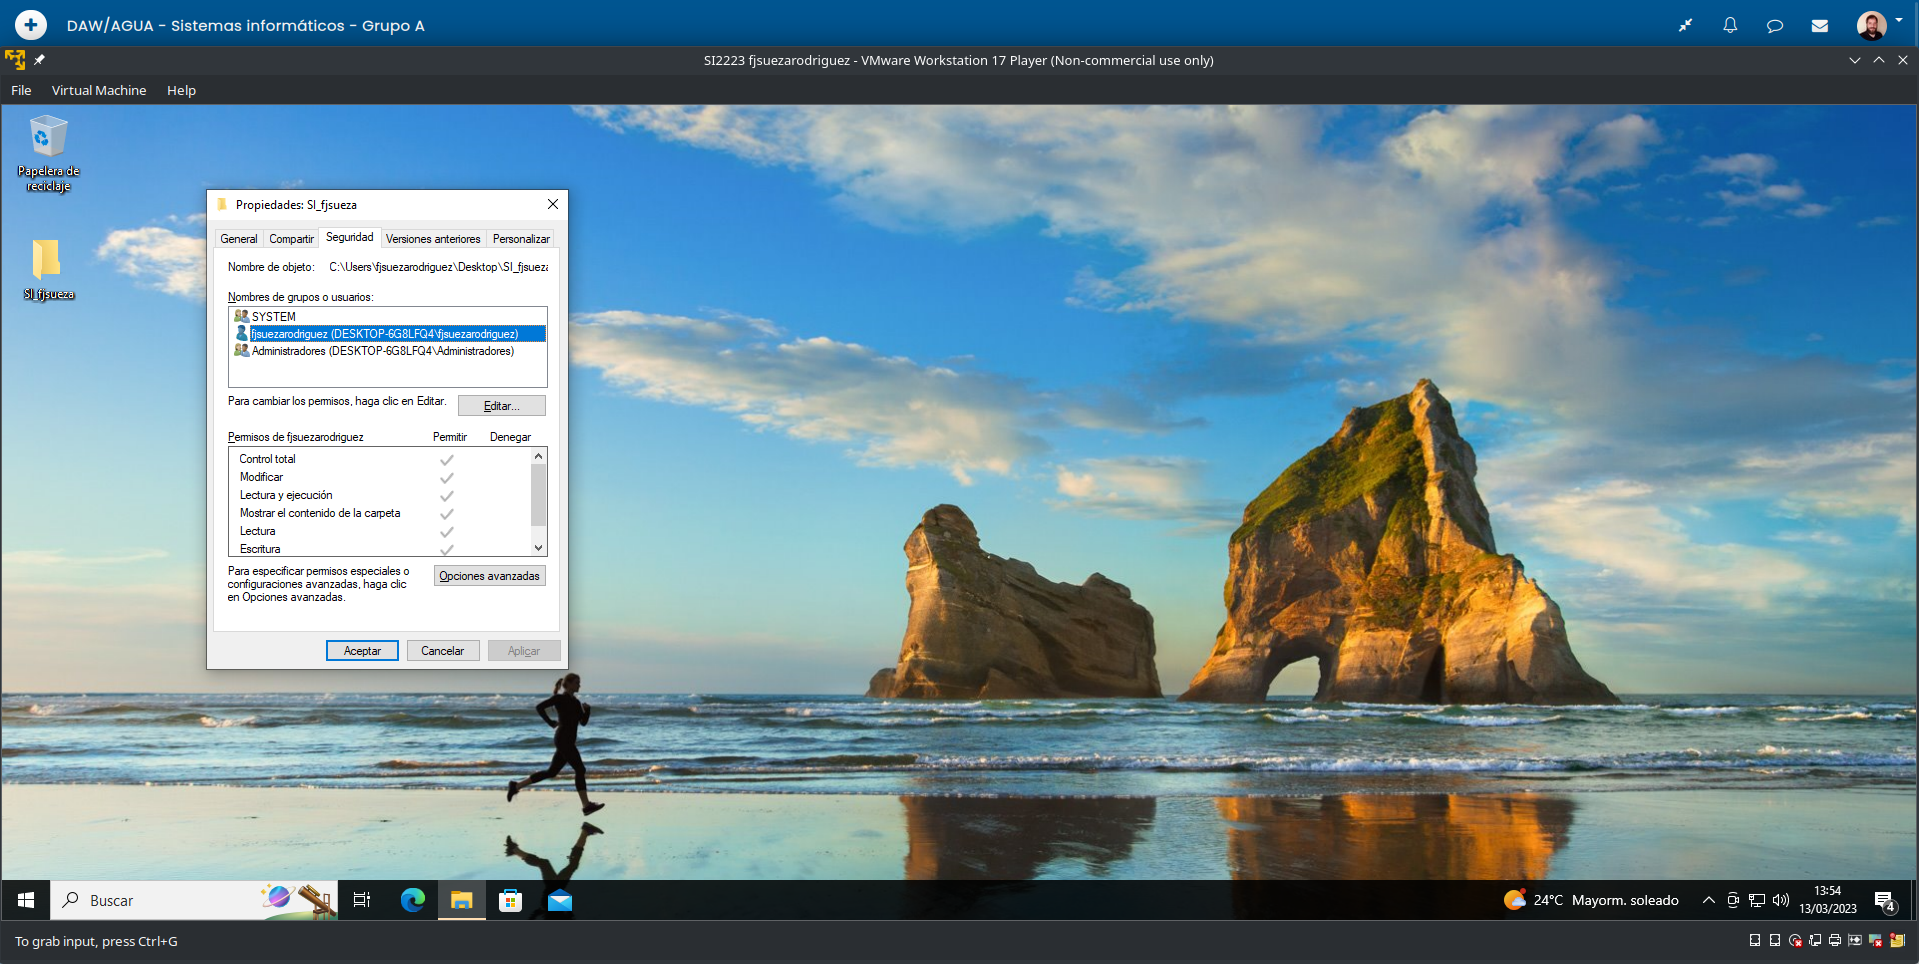
\includegraphics[scale=0.18]{ftp-1.png}
        \caption{Creación de carpeta raiz del servidor FTP}
    \end{figure}

    \item El siguiente paso consiste en activar el \textbf{servicio de FTP} en Windows 10.

    Para ello, hemos abierto el \textbf{Panel de Control} y pulsado en la opción \textbf{Programas}. En la ventana que se nos abre, hemos pulsado en la opción \textbf{Activar o desactivar características de Windows}, debajo del apartado \textbf{Programas y Características}. Se nos abrirá una nueva ventana con un conjunto de carpetas que podemos que ir desplegando y activando. En nuestro caso, nos interesa la carpeta \textbf{Internet Information Services}. Desplegamos esta carpeta y activamos \textbf{Servidor FTP}, que por defecto activará \textbf{Extensibilidad de FTP} y \textbf{Servicio FTP}. Dejaremos estas dos opciones marcadas.

    \begin{figure}[H]
        \centering
        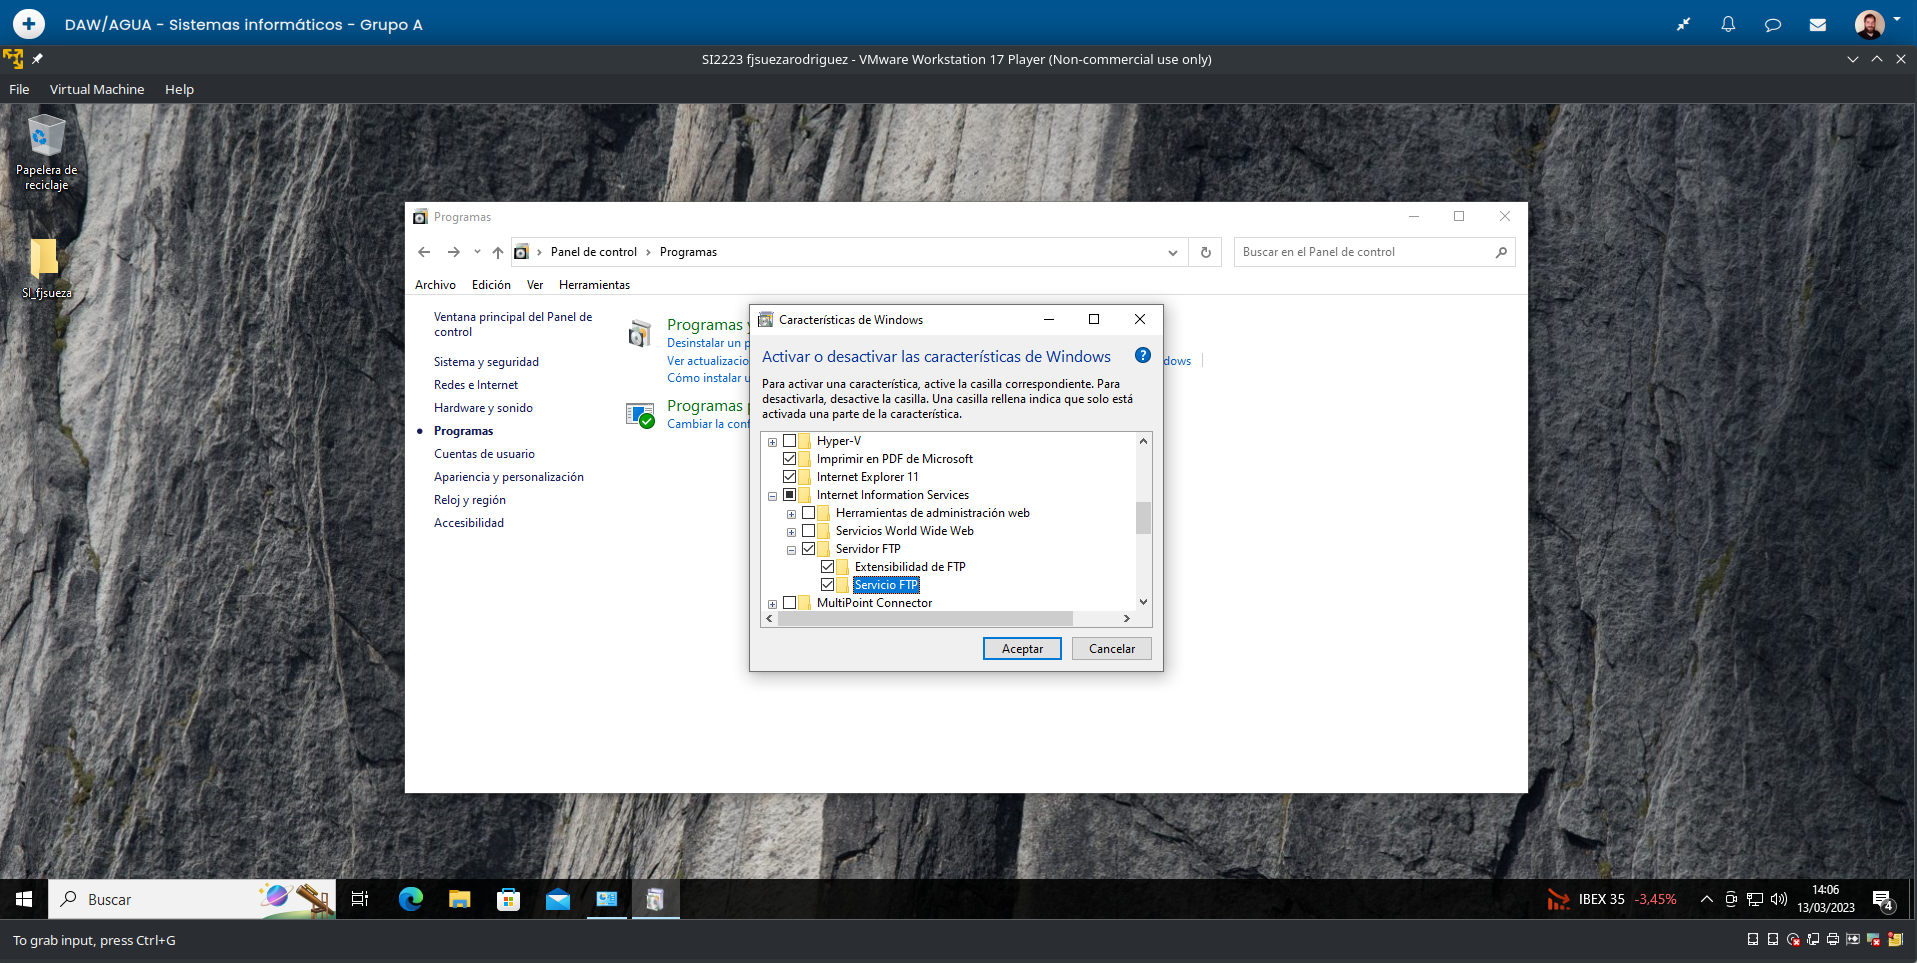
\includegraphics[scale=0.18]{ftp-2.png}
        \caption{Activación de características de Windows 10}
    \end{figure}

    \item  A continuación, vamos a crear el servidor FTP, configurando su nombre, método de autenticación, etc. Para ellos debemos acceder al \textbf{Administrador de Internet Information Services (ISS)}, al cual podemos acceder desde \textbf{Panel de Control ---> Herramientas Administrativas}.

    Una vez aquí, desplegamos el menú de la izquierda, donde figura el hostname de nuestro ordenador, y damos con el botón derecho sobre el elemento \textbf{Sitios}, pulsando sobre la opción \textbf{Agregar sitio FTP...} que se nos mostrará. Se nos abrirá una ventana donde nos guiarán en la creación del servidor FTP, permitiéndonos introducir todos los datos que se nos pide en el enunciado.

    Cabe destacar que antes del último paso, hemos \textbf{creado un certificado SSL autofirmado} usando la opción \textbf{Certificados de servidor} del administrador de Internet Information Services.

    En las siguientes capturas, podemos ver todos los datos introducidos en la creación del servidor FTP.

    \begin{figure}[H]
        \centering
        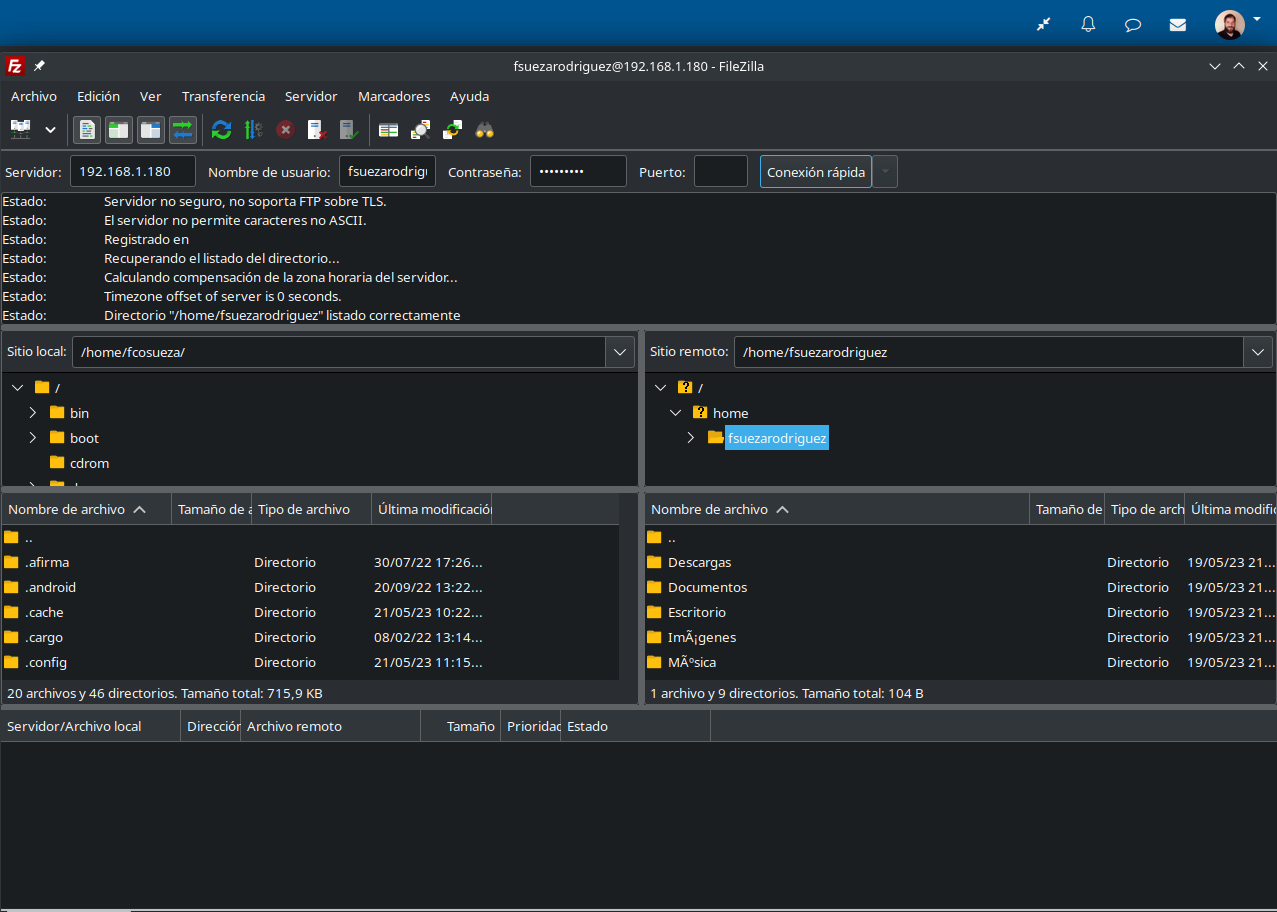
\includegraphics[scale=0.18]{ftp-3.png}
        \caption{Creación FTP: nombre y ruta}
    \end{figure}

        \begin{figure}[H]
        \centering
        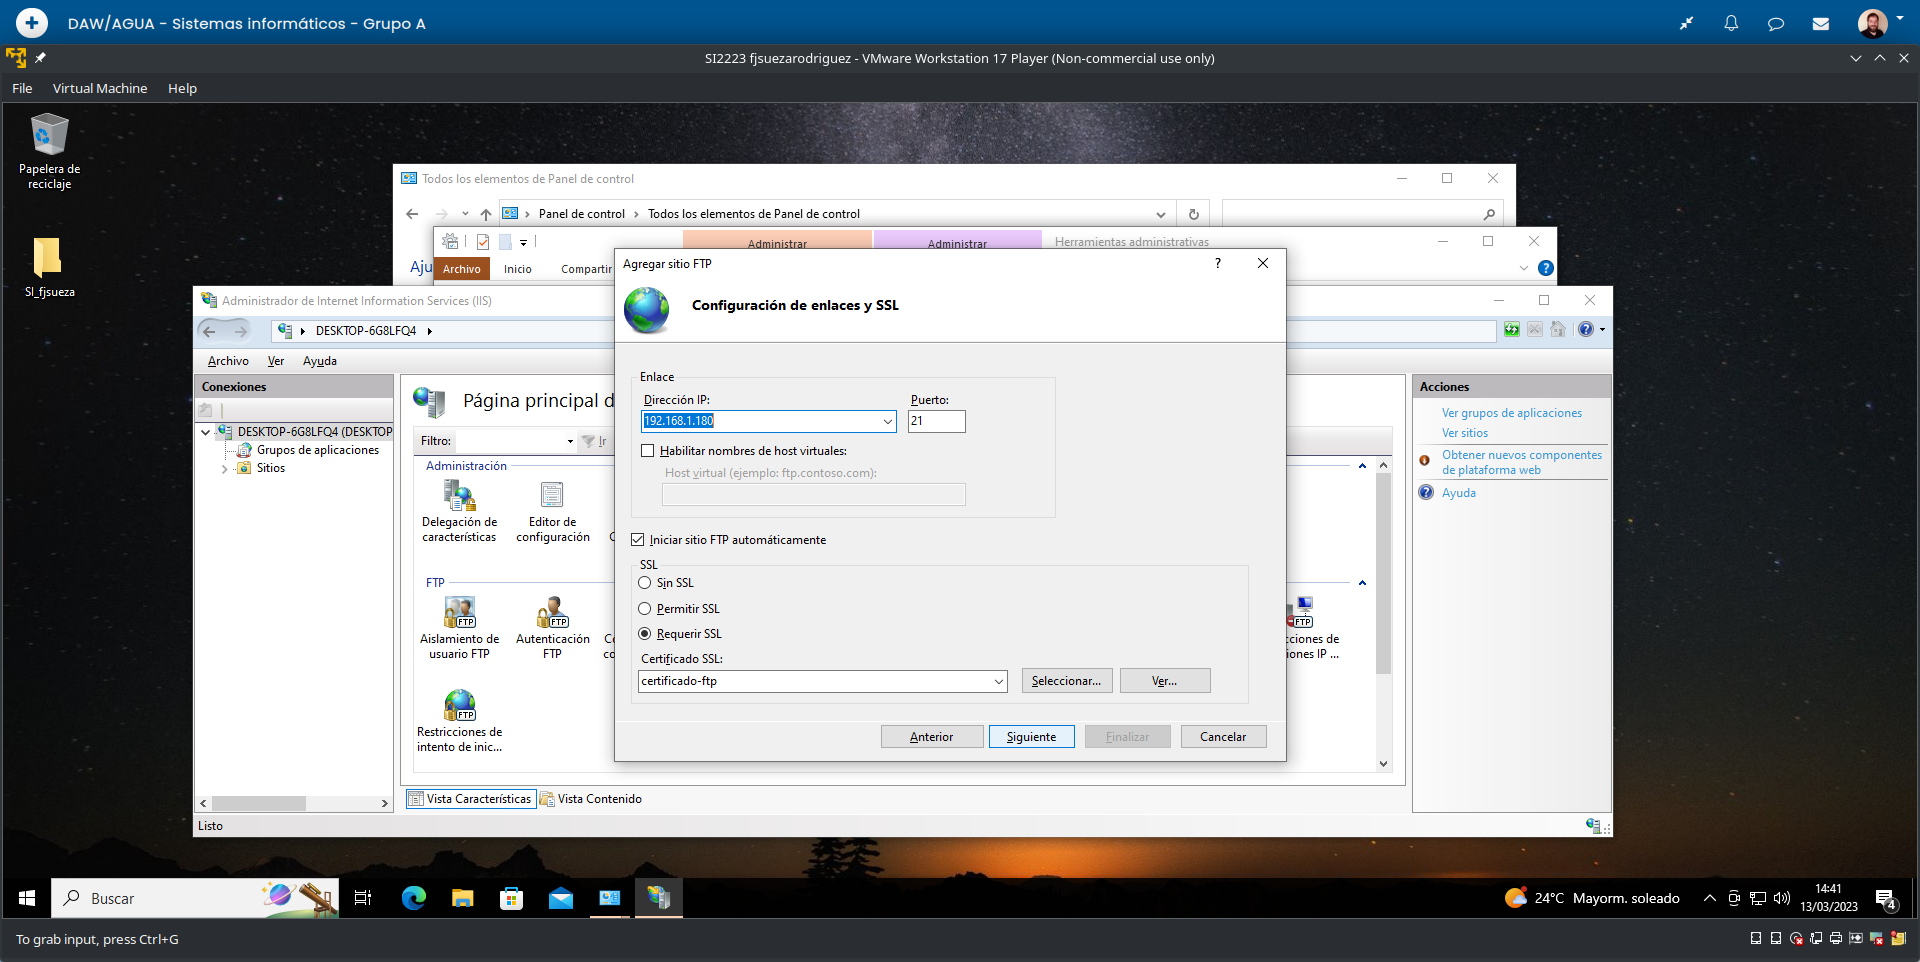
\includegraphics[scale=0.18]{ftp-4.png}
        \caption{Creación FTP: ip y certificado SSL}
    \end{figure}

    \begin{figure}[H]
        \centering
        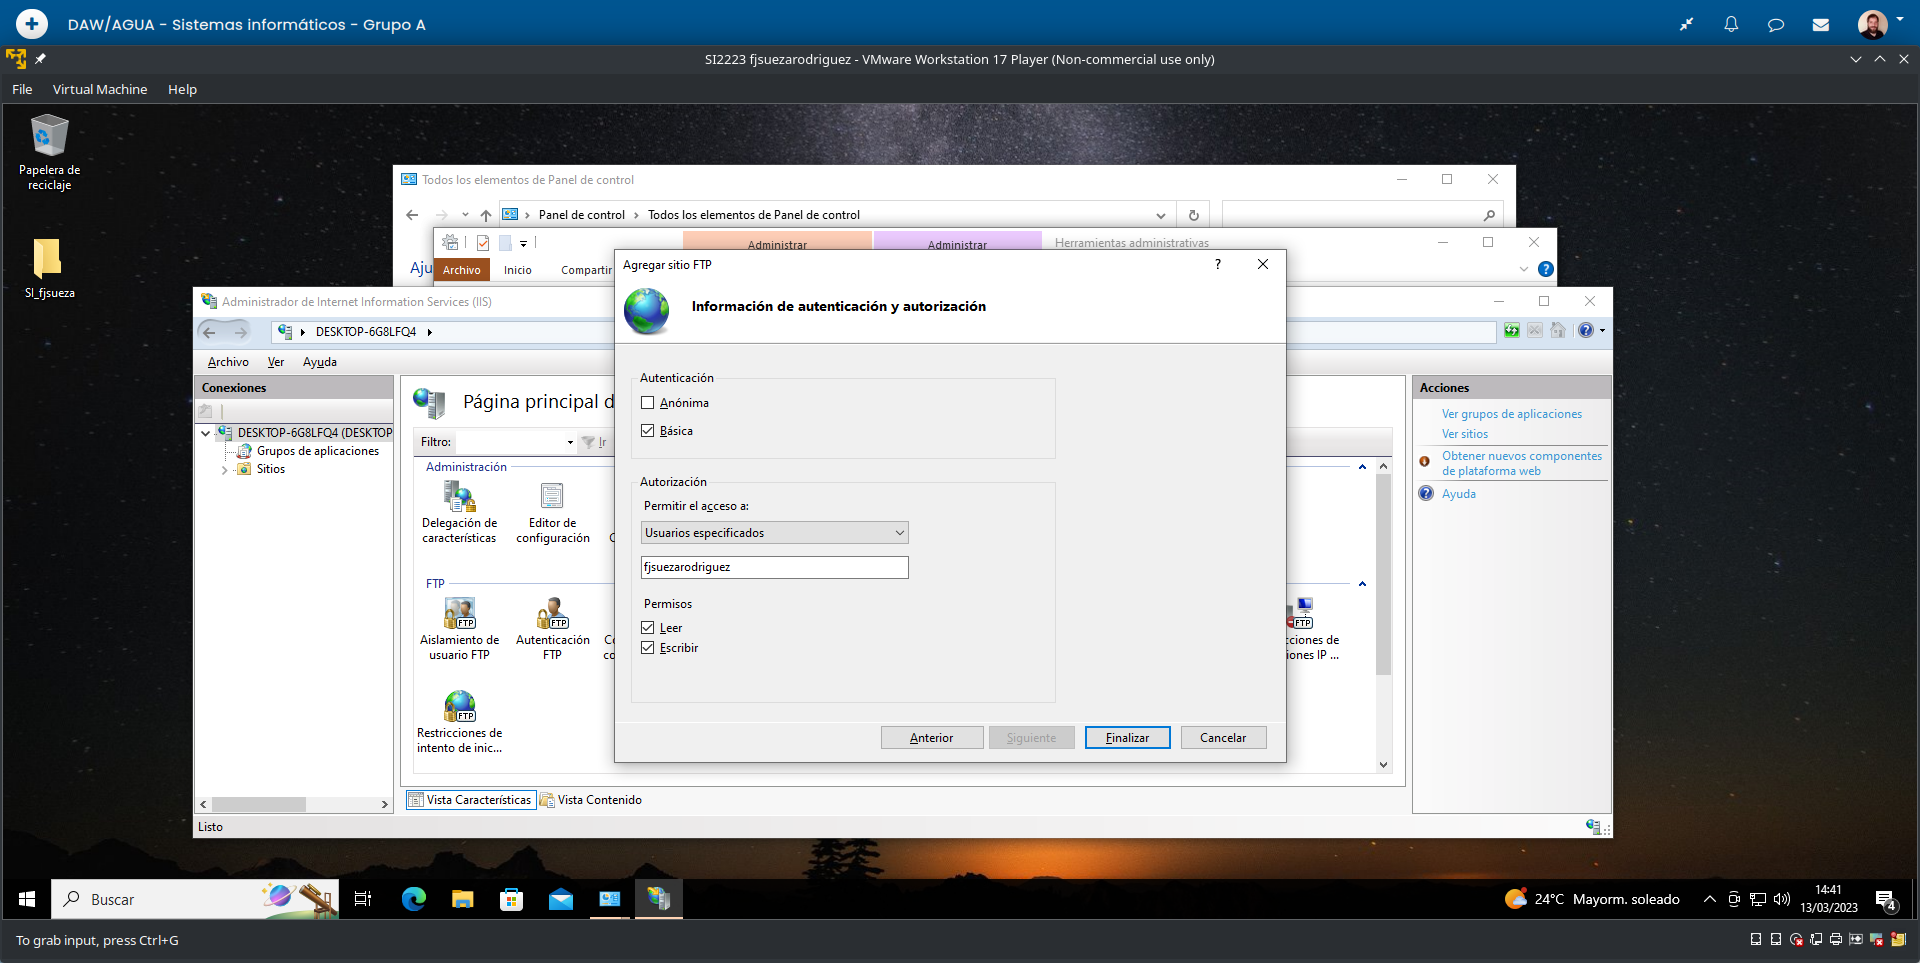
\includegraphics[scale=0.18]{ftp-5.png}
        \caption{Creación FTP: método y usuarios}
    \end{figure}

    \item Para comprobar que el servidor se ha creado correctamente, vamos a acceder a el desde el sistema anfitrión, usando la aplicación \textbf{Filezilla}. Después de introducir los datos en Filezilla, hemos \textbf{realizado la conexión correctamente}, como podemos ver en la siguiente captura.

    \begin{figure}[H]
        \centering
        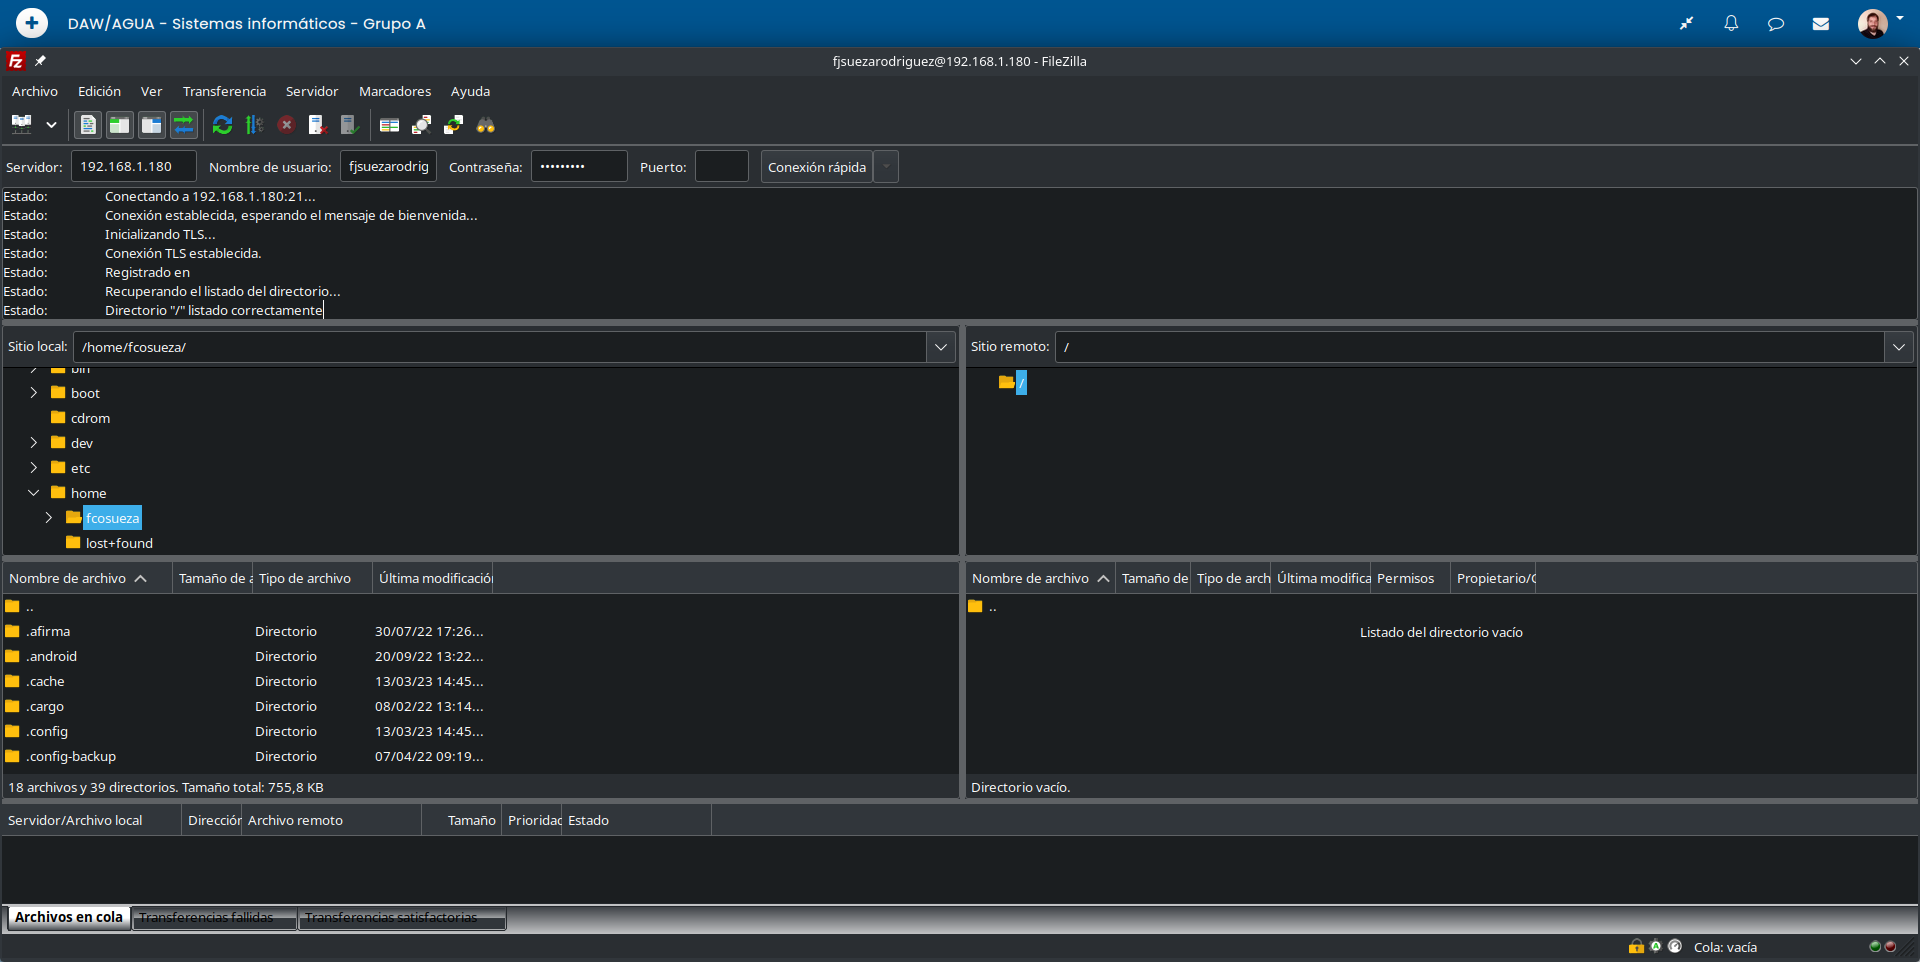
\includegraphics[scale=0.18]{ftp-6.png}
        \caption{Conexión al FTP desde la máquina anfitrión en Filezilla}
    \end{figure}

    \item Por último, hemos creado una imagen de mapa de bits en el directorio del FTP, para descargarla con el cliente, y hemos también subido un libro al FTP. Las dos operaciones se han realizado con éxito, como podemos ver en la siguiente captura.

    \begin{figure}[H]
        \centering
        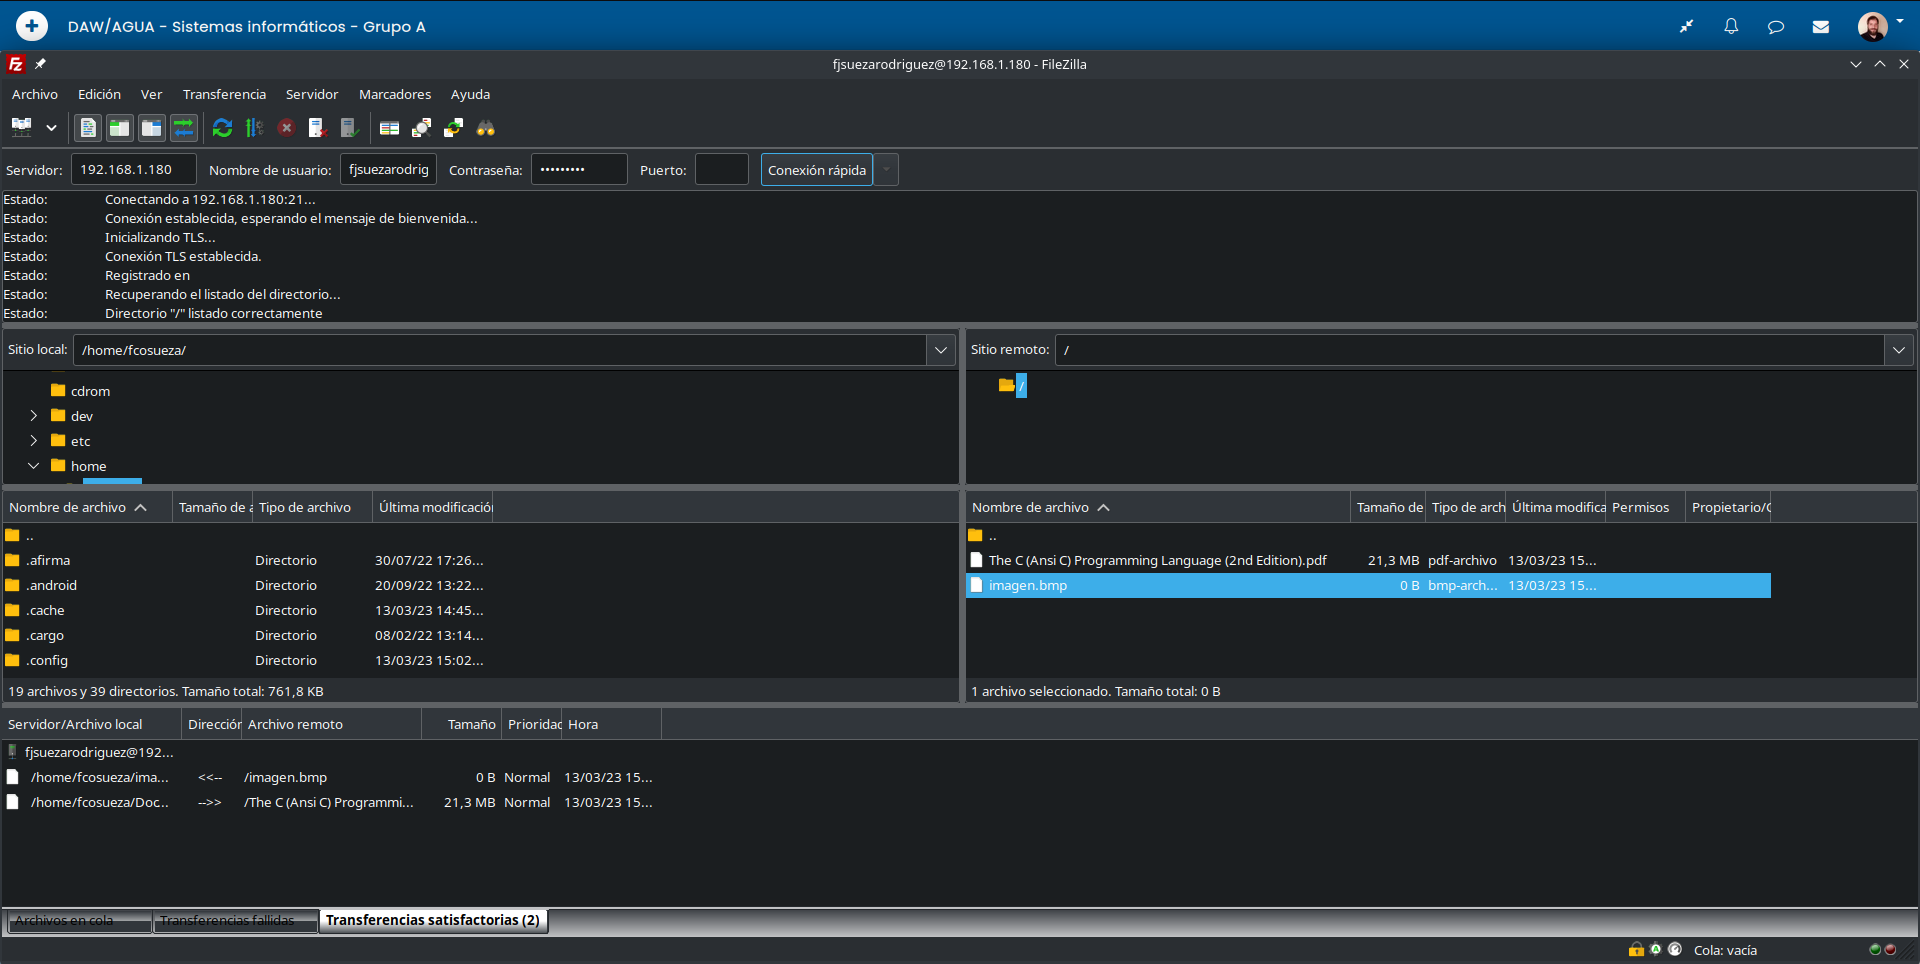
\includegraphics[scale=0.18]{ftp-7.png}
        \caption{Descarga y subida de archivos al servidor FTP desde Filezilla}
    \end{figure}
\end{enumerate}

\subsection{Actividad 4: Servidor Web en Windows 10}

\subsubsection{Enunciado}
Instala y configura el entorno de servidor web ``XAMPP'' en la MV. Una vez activados los servicios, en la carpeta pública del servidor Apache (``htdocs'') crea una carpeta llamada ``miweb'', en la cual guardarás una fotografía tuya  y un archivo ``.html'' con el siguiente código:

\begin{figure}[H]
    \centering
    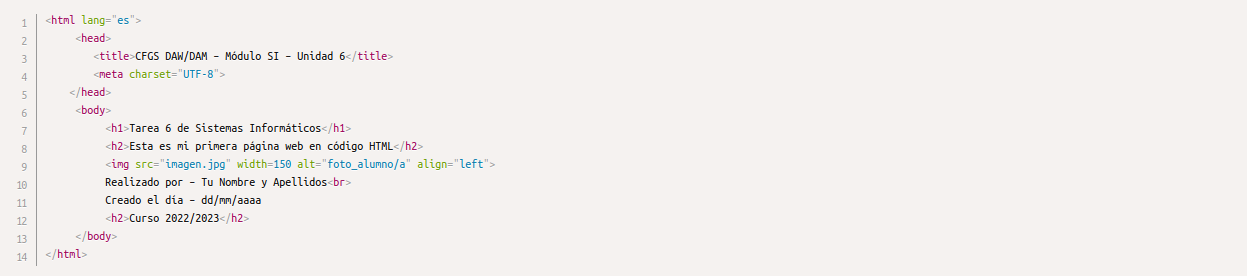
\includegraphics[scale=0.50]{codigo-web.png}
    \caption{Código de la página web}
\end{figure}

Para ello, abre un editor simple de texto, copia las líneas de código HTML personalizándolo con tu nombre y referenciando la imagen correctamente. Por último, guarda el archivo como ``miprimeraweb.html'' en la carpeta ``miweb'' y añade a la misma una foto tuya de tamaño carnet para que se visualice al abrir la página.

A continuación accede a dicha página web desde un navegador web en la máquina anfitriona usando esta URL: ``http://<IP\_de\_la\_MV>/miweb/miprimeraweb.html''.

Recuerda, el acceso será desde la máquina anfitriona (navegador web) a la MV (servidor web).

\textbf{Capturas}:

\begin{itemize}
    \item XAMPP instalado y con el servicio Apache en marcha.
    \item Creación del archivo ``miprimeraweb.html'' en un editor de texto (se debe ver el código HTML).
    \item Archivo ``miprimeraweb.html'' y archivo de fotografía situados en la carpeta ``miweb''.
    \item Acceso a la página web creada desde un navegador web en la máquina anfitriona (se debe ver en la barra de direcciones la URL que se ha usado para acceder).
\end{itemize}

\subsubsection{Solución}
En este ejercicio vamos a instalar el bundle \textbf{XAMPP}, que nos permite instalar al mismo tiempo \textbf{Apache} con \textbf{MySQL}, \textbf{PHP} y \textbf{Perl}.

\begin{enumerate}
    \item En primer lugar, hemos descargado XAMPP desde \href{https://www.apachefriends.org/es/index.html}{su página oficial} y hemos procedido a instalarlo, mediante el instalador que nos hemos descargado.

    Una vez instalado, se ha abierto el \textbf{Panel de Control de XAMPP} y hemos activado el servidor web \textbf{Apache}, como podemos ver en la siguiente imagen.

    \begin{figure}[H]
        \centering
        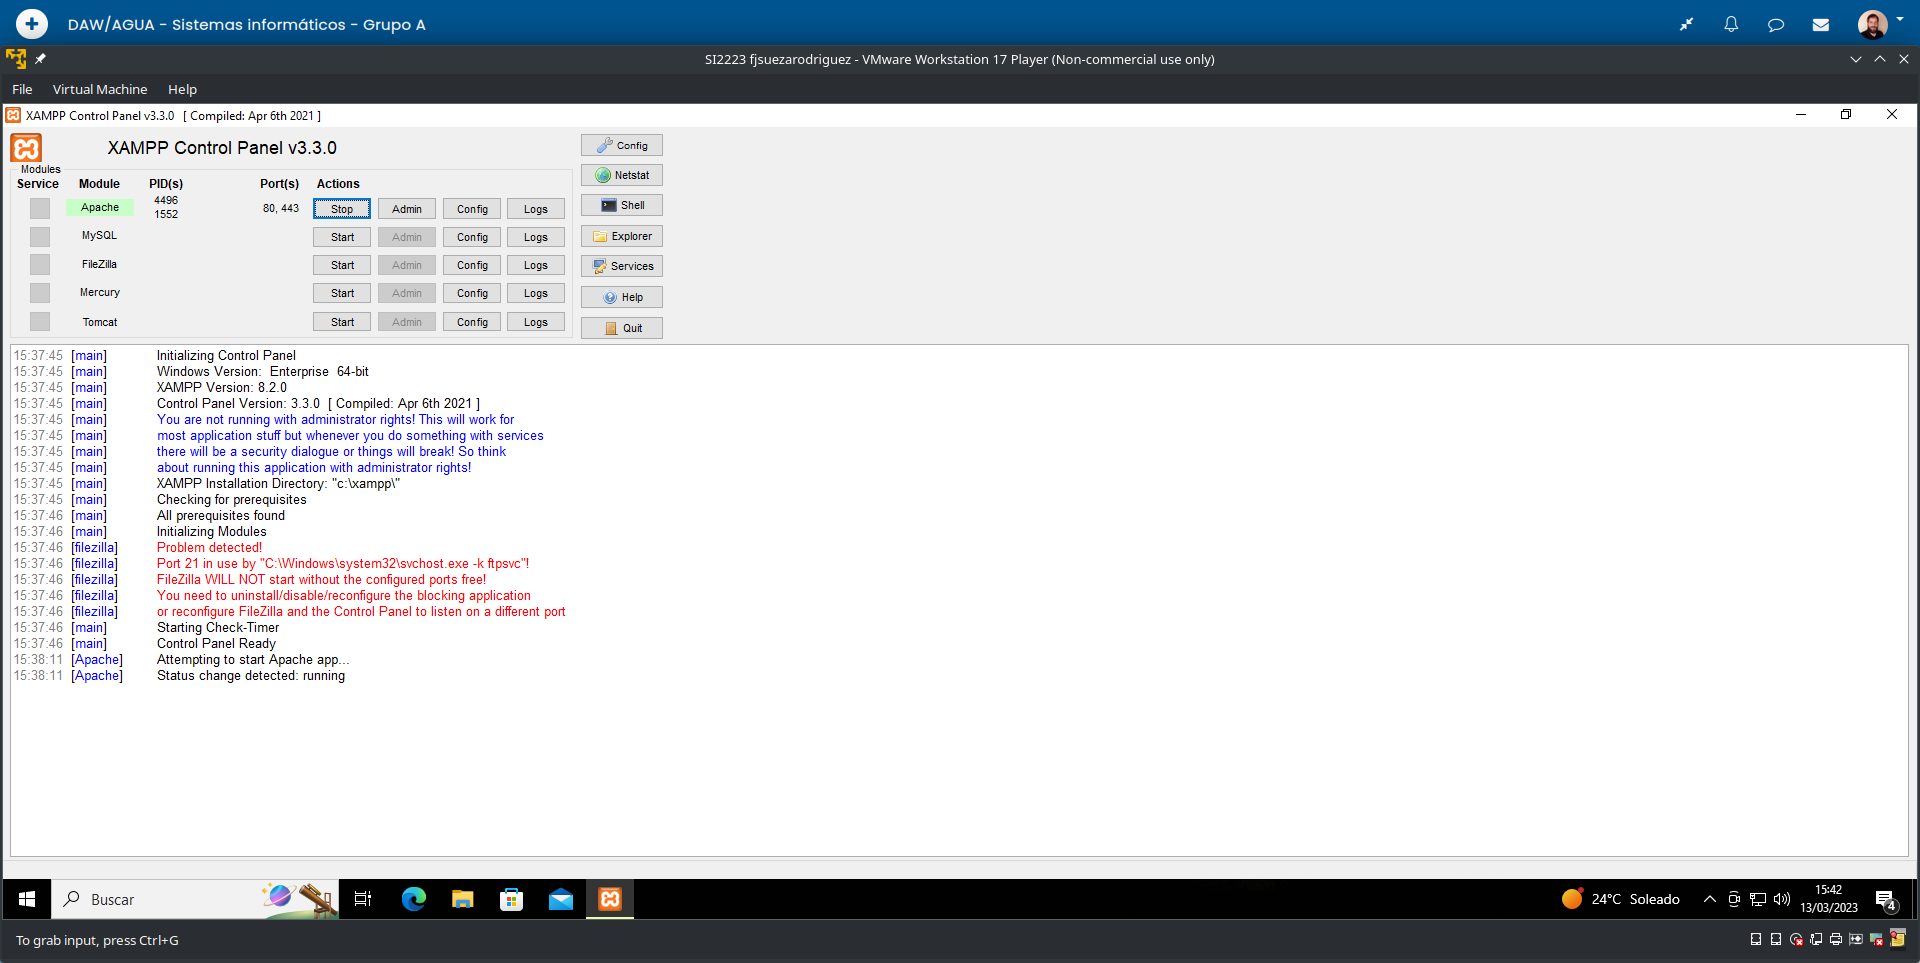
\includegraphics[scale=0.18]{web-server-1.png}
        \caption{XAMPP instalado y con Apache ejecutándose}
    \end{figure}

    \item Una vez instalado correctamente XAMPP, hemos creado la que será nuestra página de prueba, usando para el \textbf{Notepad}, ya que es una web muy sencilla y no necesitamos editores mas complejos. En la siguiente imagen se muestra el código creado en Notepad.

    \begin{figure}[H]
        \centering
        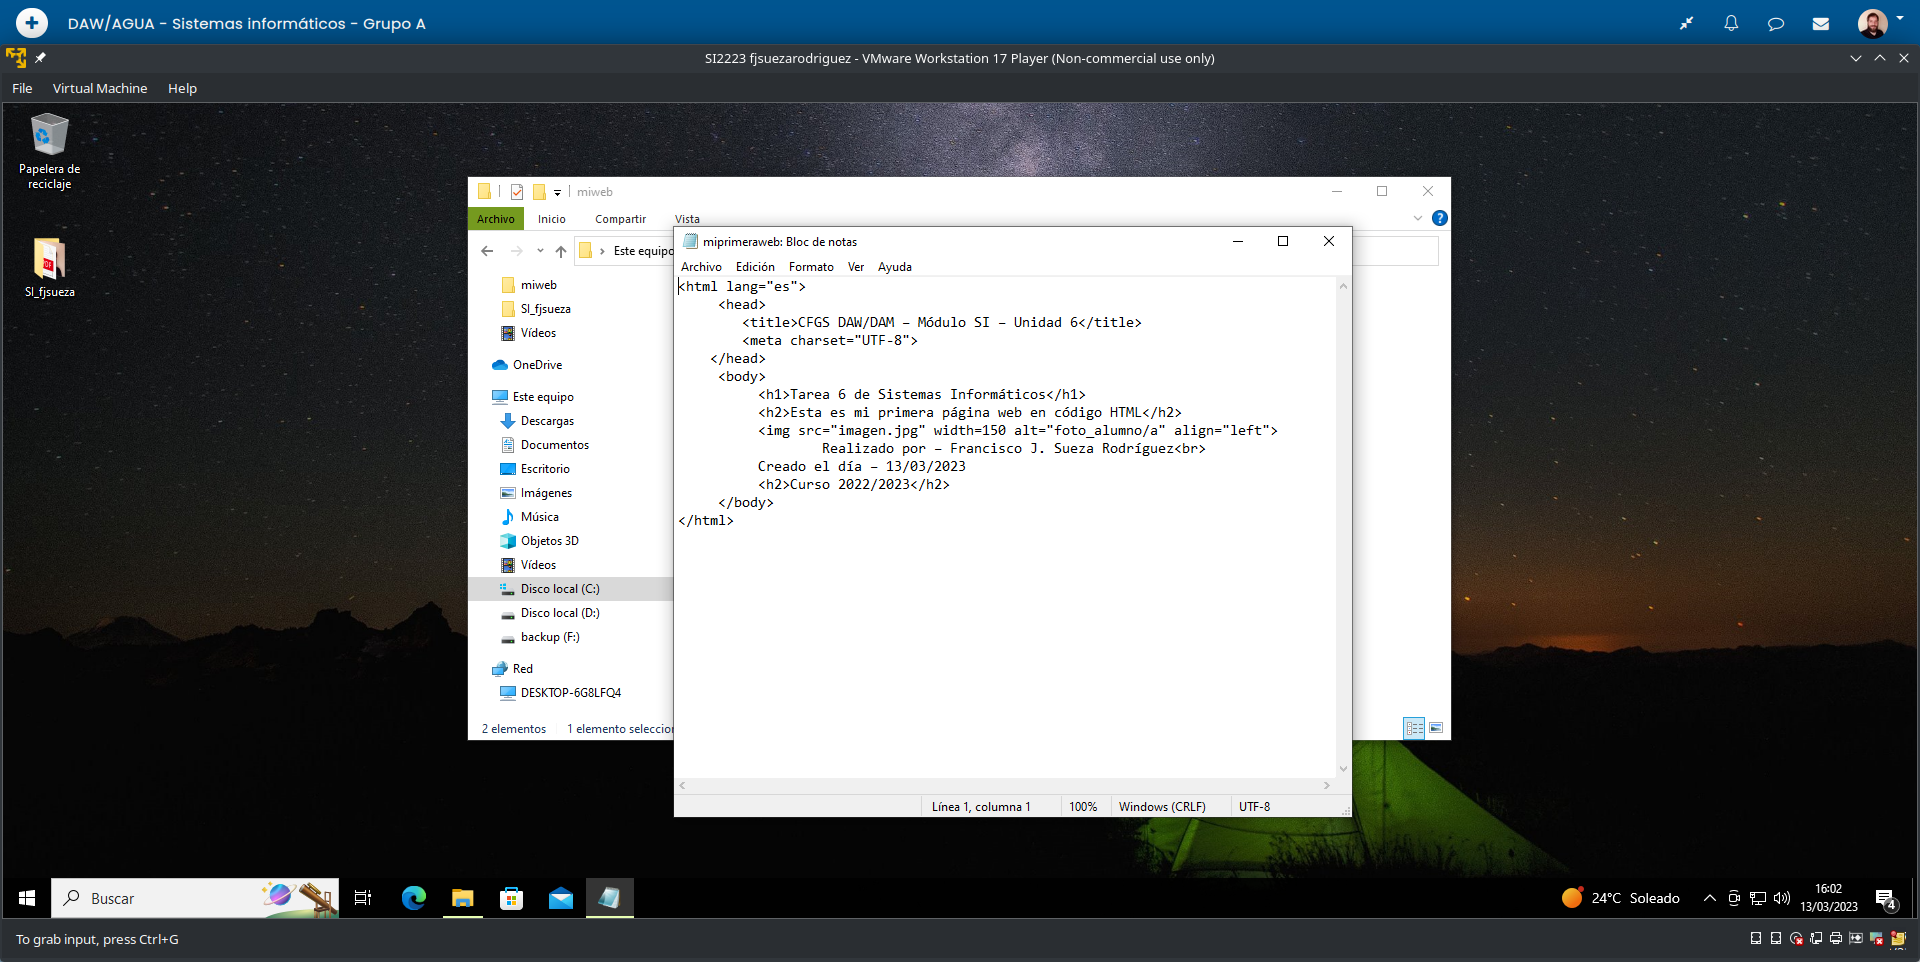
\includegraphics[scale=0.18]{web-server-2.png}
        \caption{Creación del fichero HTML}
    \end{figure}

    \item Hemos creado un directorio dentro del directorio \textbf{htdocs}, llamado \textbf{miweb}, y hemos agregado el archivo HTML creado en el paso anterior y una imagen personal tamaño carnet.

    \begin{figure}[H]
        \centering
        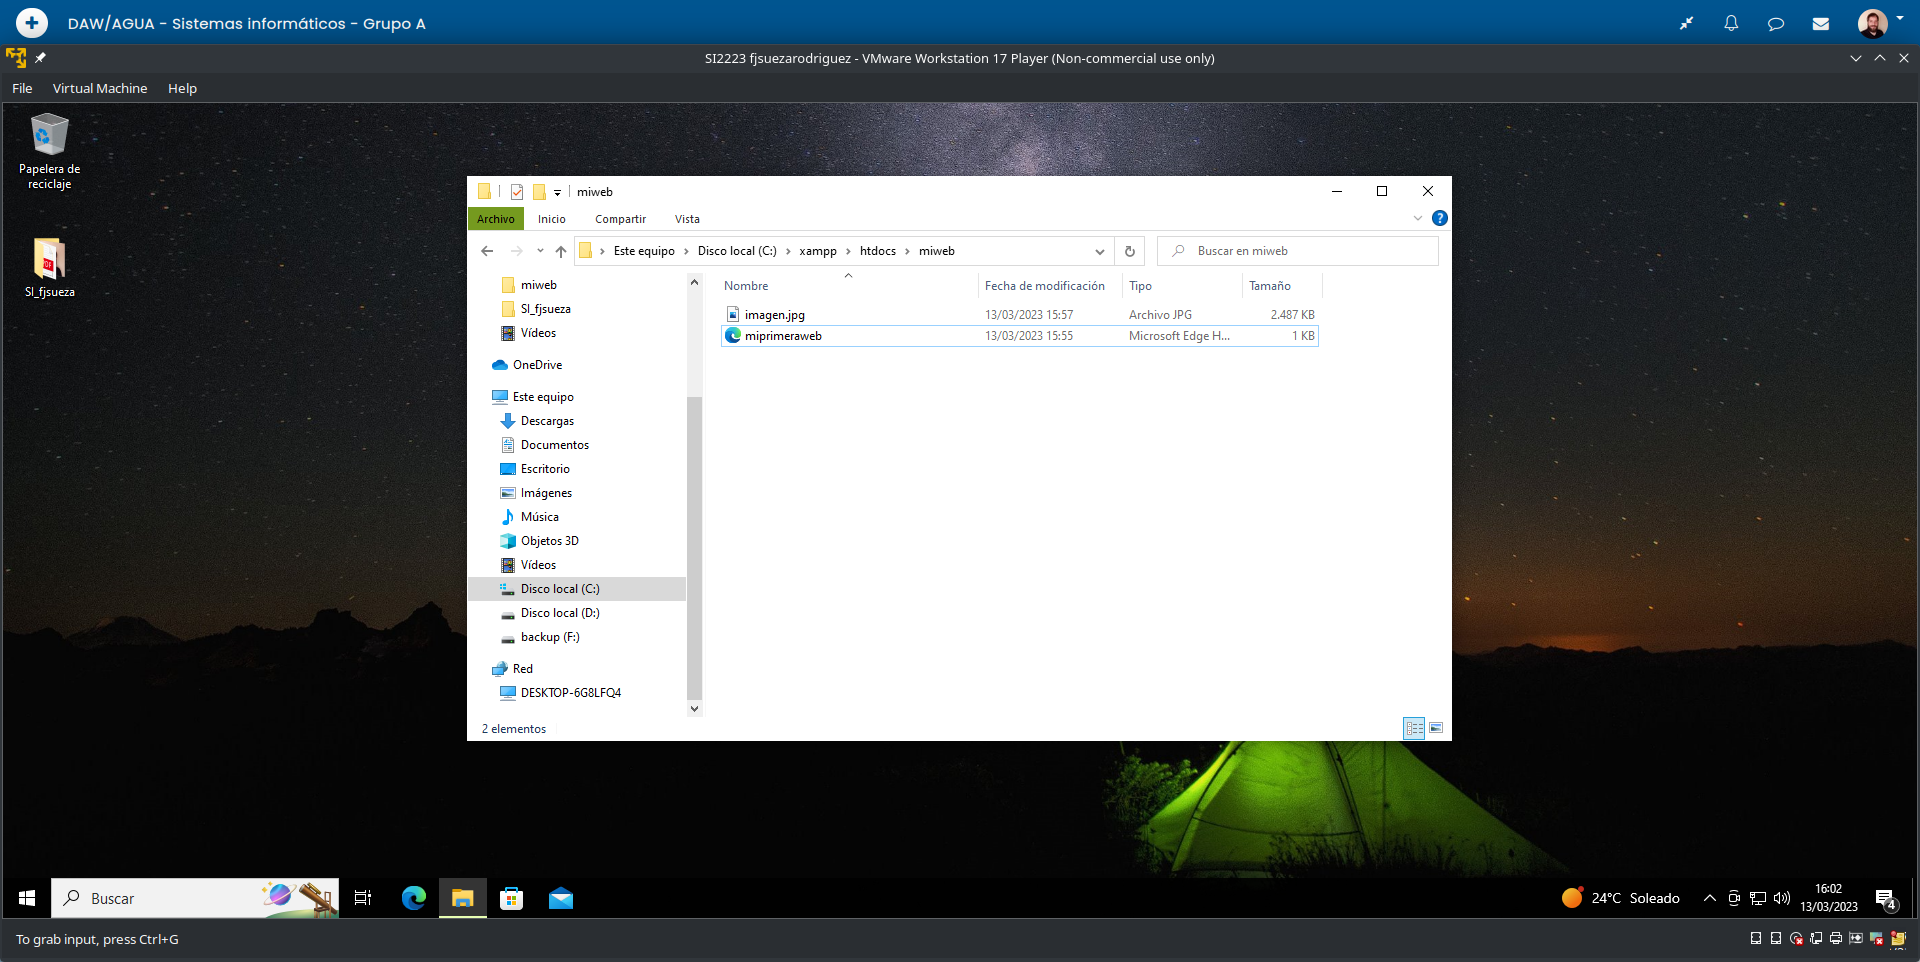
\includegraphics[scale=0.18]{web-server-3.png}
        \caption{Archivos dentro de la carpeta miweb}
    \end{figure}

    \item Por último, hemos\textbf{ accedido a la página web} creada desde el el sistema anfitrión, específicamente desde el navegador web Firefox. En la siguiente captura, se puede ver el acceso a la página a través de la red.

    \begin{figure}[H]
        \centering
        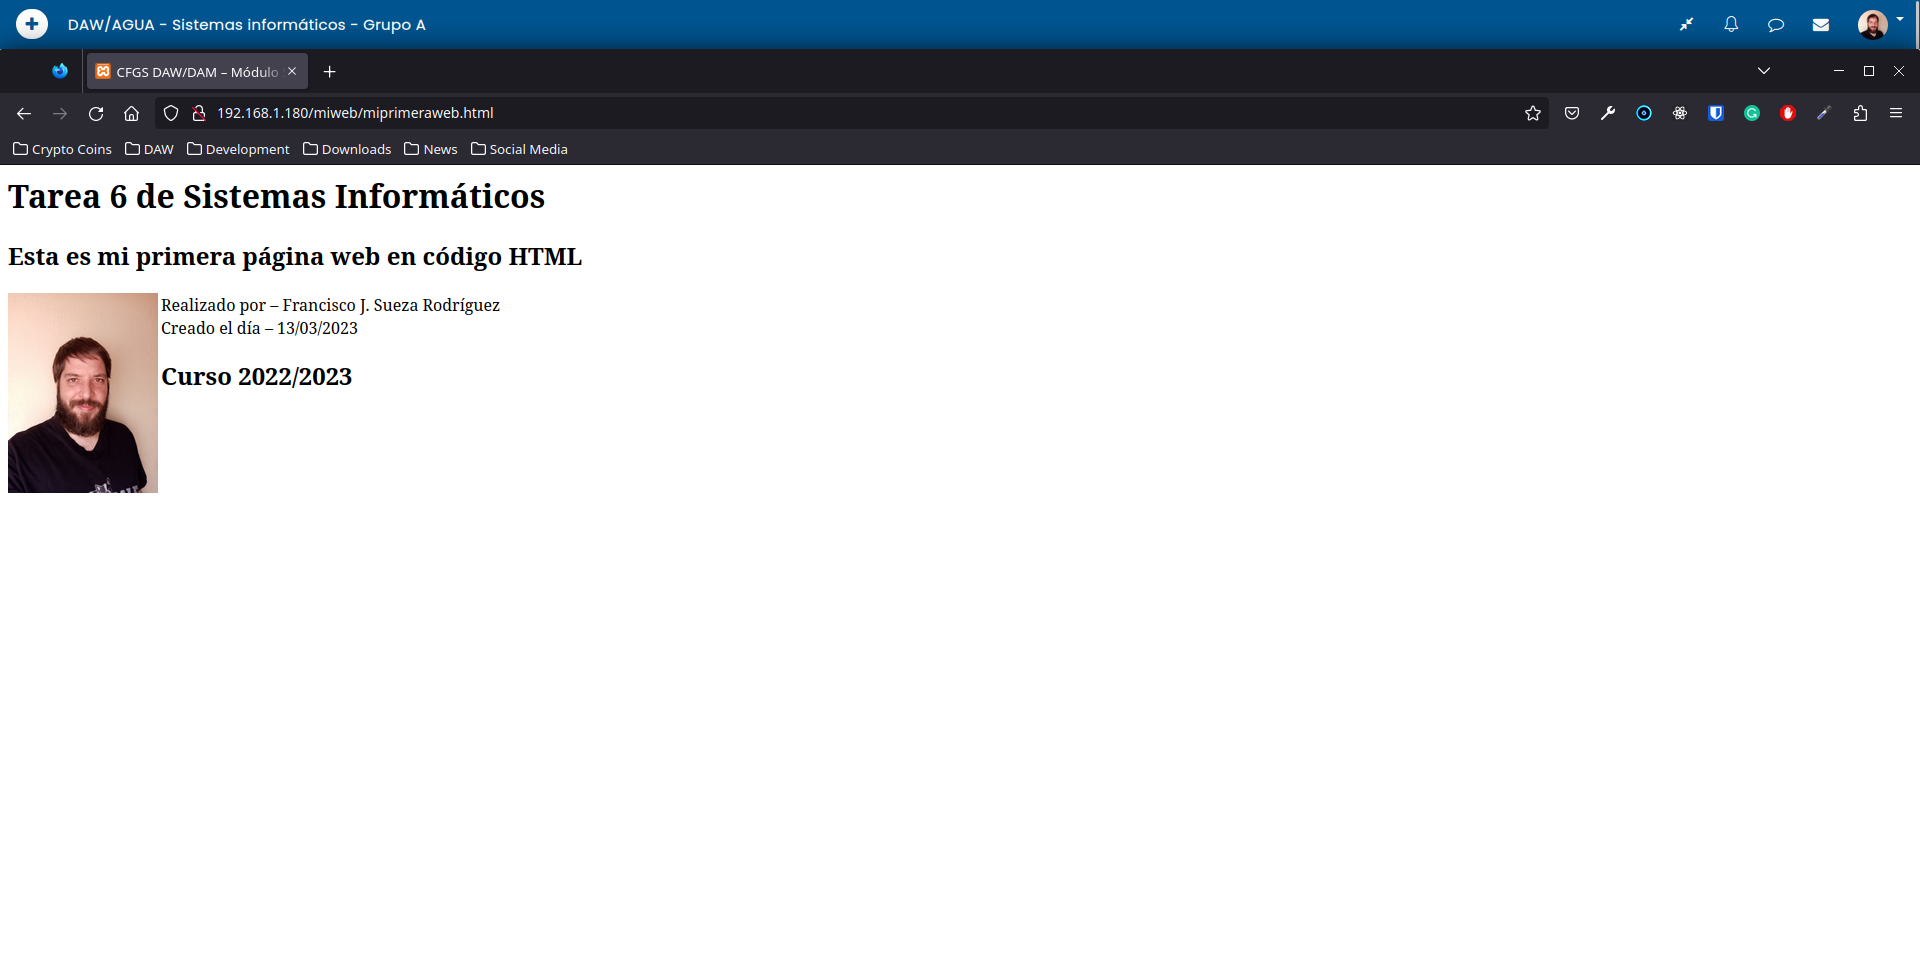
\includegraphics[scale=0.18]{web-server-4.png}
        \caption{Acceso a la página web desde el sistema anfitrión}
    \end{figure}
\end{enumerate}

\subsection{Actividad 5: Utilización de Antivirus}

\subsubsection{Enunciado}
Utilizando un antivirus, realiza lo siguiente:

\begin{enumerate}
    \item Analiza una memoria USB que tengas conectada al ordenador. Comenta el resultado del análisis y qué se haría en caso de haber encontrado alguna amenaza.
    \item Configura un análisis completo programado para que se ejecute semanalmente todos los lunes a las 5:00 horas. Nombra la tarea como 'ANÁLISIS SEMANAL - <tu nombre completo y apellidos>'.
\end{enumerate}

Para hacer esta actividad necesitas tener instalado un programa antivirus o puedes utilizar el propio "Windows Defender" incluido con Windows 10. Estos son algunos antivirus gratuitos que puedes instalar:

\begin{itemize}
    \item Avast! Free Antivirus.
    \item Avira Free Antivirus.
    \item AVG Anti-virus Free Edition.
\end{itemize}

\textbf{Capturas}:

\begin{itemize}
    \item Acción para iniciar el análisis de la memoria USB.
    \item Resultado del análisis de dicha memoria.
    \item Programación del análisis semanal.
\end{itemize}

\subsubsection{Solución}
En este punto vamos a utilizar un \textbf{antivirus} para \textbf{analizar una memoria usb} y también vamos a \textbf{configurar análisis semanales} para mantener nuestro sistema seguro y libre virus. Nosotros hemos optado por usar \textbf{Windows Defender}, ya que es el software que viene por defecto en Windows 10.

\begin{enumerate}
    \item En primer ligar hemos analizado un dispositivo USB. En nuestro caso, no contábamos con ningún pendrive, así que hemos conectado un \textbf{disco duro externo Seagate de 1 TB}.

    Una vez conectado el disco,  hemos abierto el \textbf{Explorador de archivos} y pulsado con el botón derecho sobre el dispositivo conectado, llamado \textbf{Multimedia} y con la letra \textbf{G} asignada. Cuando se despliega el menú contextual, podemos seleccionar la opción \textbf{Examinar con Windows Defender}, que una vez pulsada iniciará automáticamente un análisis de la unidad.

    \begin{figure}[H]
        \centering
        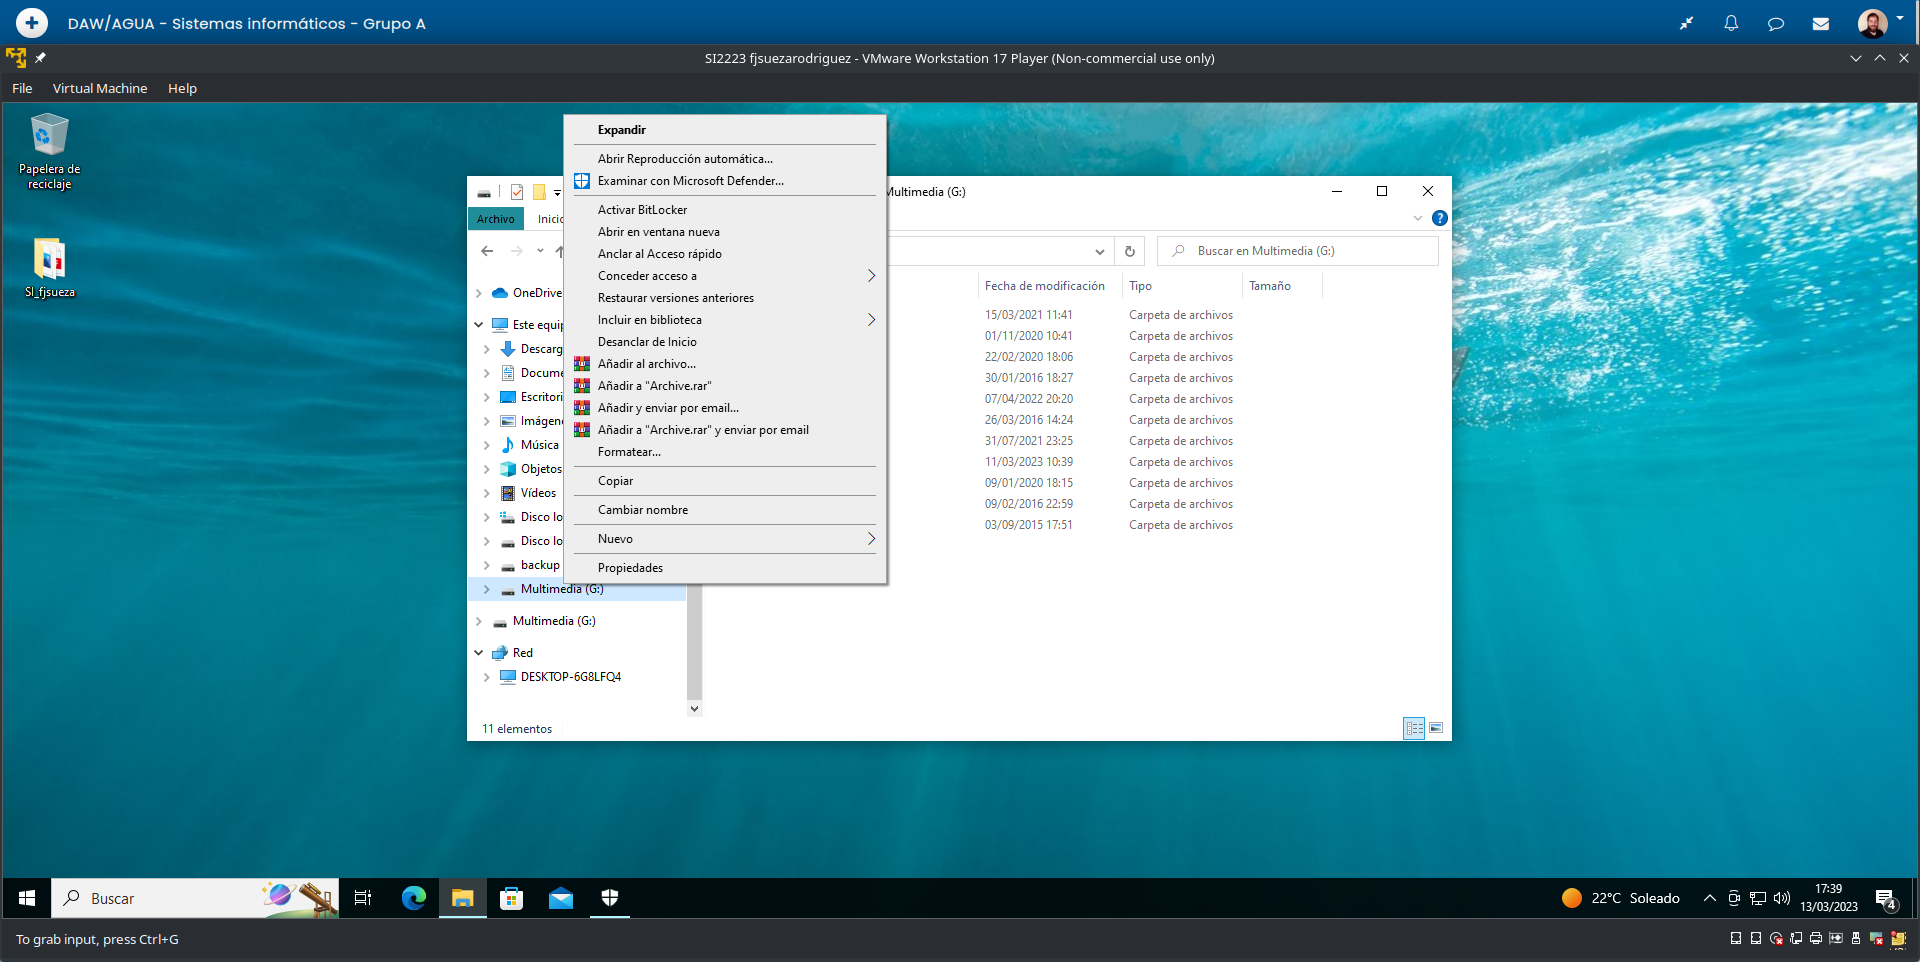
\includegraphics[scale=0.18]{antivirus-1.png}
        \caption{Menu contextual de la unidad USB conectada}
    \end{figure}

    \item Una vez realizado el examen, se nos ha notificado que \textbf{no existen amenazas}, pero en el caso de que las existieran, Windows Defender nos daría diferentes acciones a realizar, siendo las principales \textbf{eliminar los archivos infectados} o \textbf{poner estos en cuarentena}. En la siguiente imagen, vemos el resultado del análisis.

    \begin{figure}[H]
        \centering
        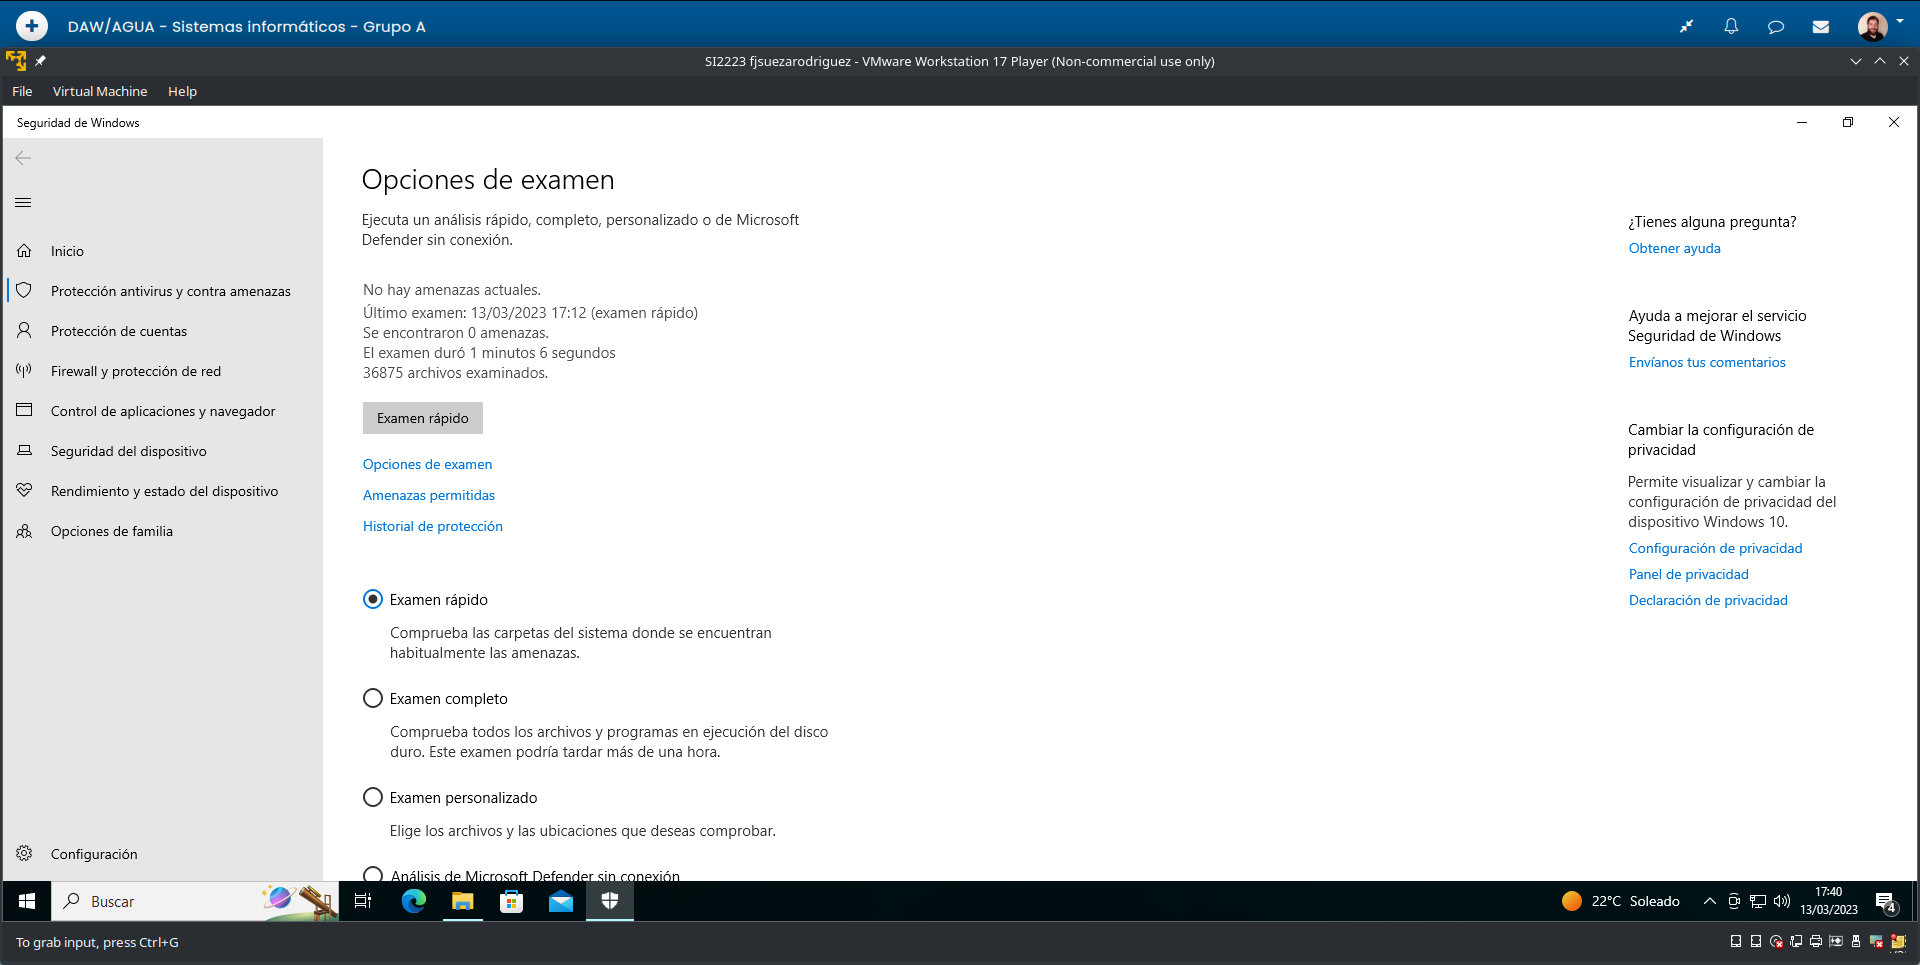
\includegraphics[scale=0.18]{antivirus-2.png}
        \caption{Resultado del análisis del dispositivo USB}
    \end{figure}

    \item Por último, vamos a \textbf{programar una tarea} para que Windows Defender realice un análisis del sistema todos \textbf{Lunes a las 5:00h}. Para ello, en primer lugar, hemos abierto el \textbf{Programador de Tareas}. En la \textbf{Biblioteca el Programador de Tareas} en el apartado \textbf{Microsoft}, buscamos y seleccionamos la carpeta de \textbf{Windows Defender}.

    Desde aquí, podemos crear la nueva tarea, añadiendo un \textbf{desencadenador} para que se ejecute en la fecha deseada e indicando que se debe ejecutar la aplicación \textbf{Windows Defender Scheduled Scan}. Además de el resto de datos. En la siguiente imagen se puede ver la tarea ya correctamente programada.

    \begin{figure}[H]
        \centering
        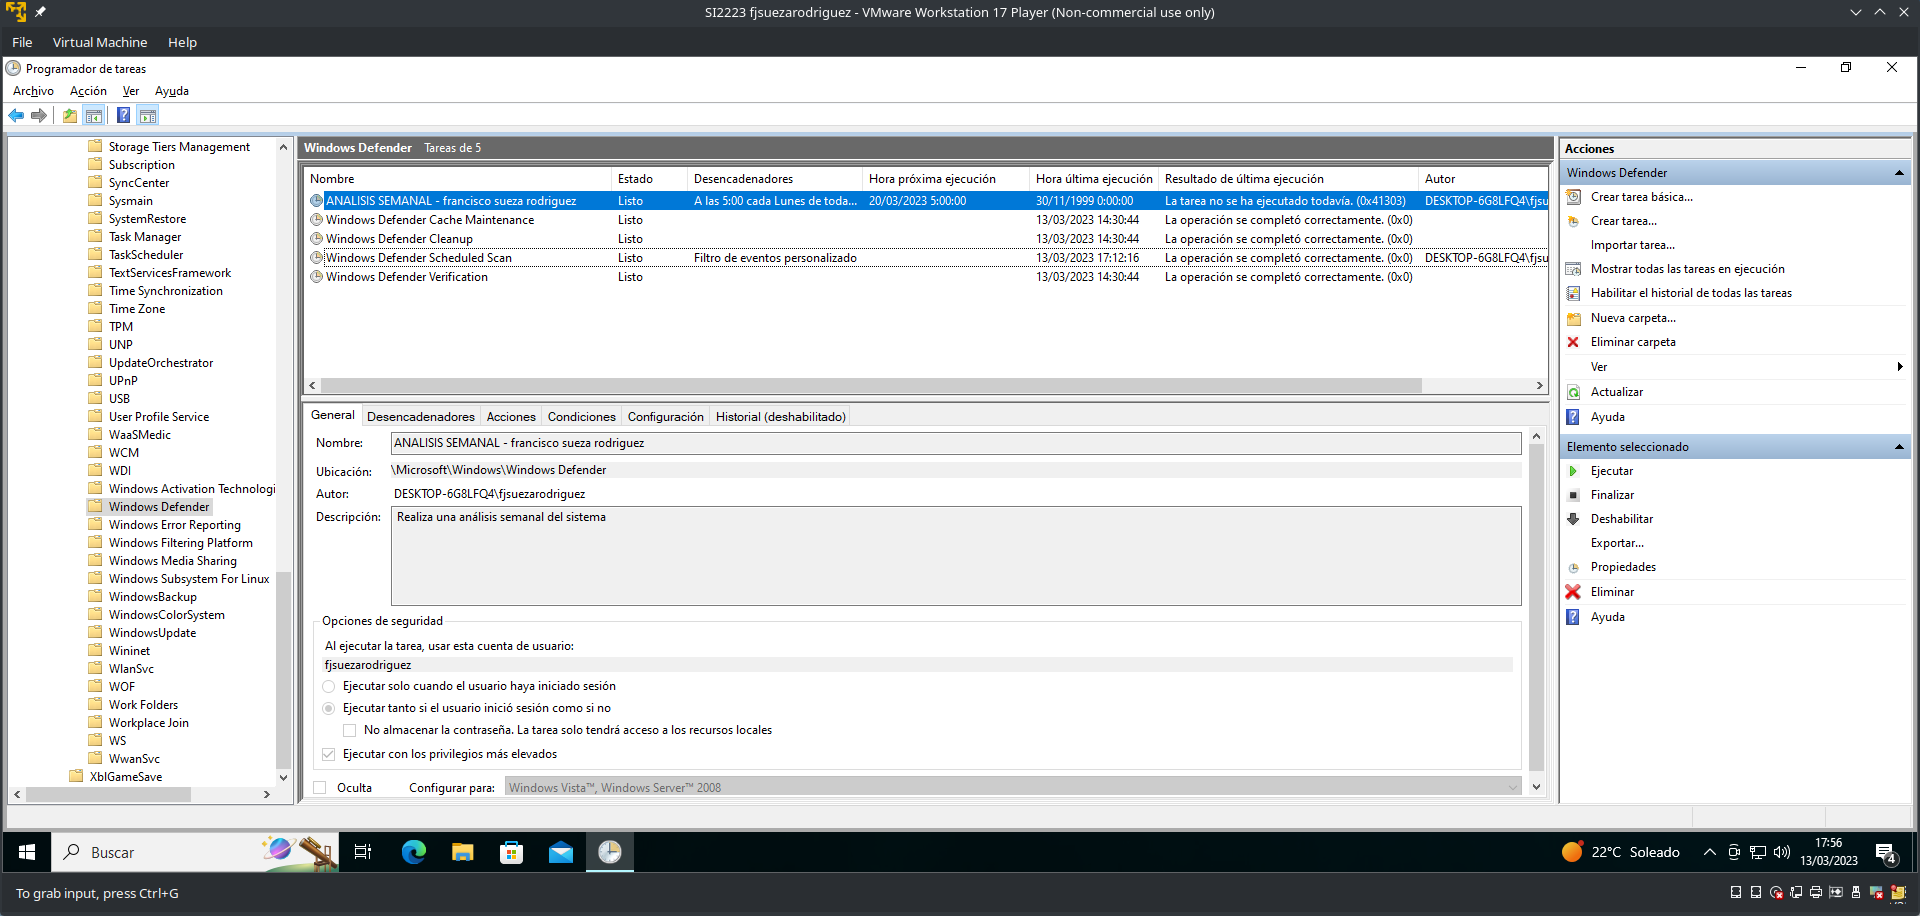
\includegraphics[scale=0.18]{antivirus-3.png}
        \caption{Tarea para el análisis semanal con Windows Defender programada}
    \end{figure}
\end{enumerate}

\subsection{Actividad 6: Configuración de la Red Wi-Fi en un Router Inalámbrico y Conexión}

\subsubsection{Enunciado}
Accede a un punto de acceso o router inalámbrico y muestra cómo se realizarían las siguientes operaciones:

\begin{enumerate}
    \item Configuración de la clave de acceso al panel de configuración del router.
    \item Configuración de la clave de red inalámbrica. Si aún no dispones de clave, establécela.
    \item Configuración del tipo de cifrado. Cambia el cifrado a WPA2-Personal si no lo tienes así.
    \item Muestra cómo se activaría el filtrado de direcciones MAC para los equipos de tu red. Averigua la dirección MAC del equipo que estés usando o un dispositivo móvil de tu red y explica cómo se añadiría a la lista de filtrado por MAC. No es necesario que apliques y guardes estos cambios, basta con explicarlo y mostrar las ventanas donde se realiza.
\end{enumerate}

\textbf{Capturas}:

\begin{itemize}
    \item Acceso al punto de acceso inalámbrico a través de un navegador web (se debe ver la URL usada para acceder).
    \item Configuración de la clave de acceso al panel de configuración del router.
    \item Configuración de la clave de red inalámbrica.
    \item Configuración del cifrado en WPA2-Personal.
    \item Dirección MAC del equipo que estás usando o de otro equipo de tu red.
    \item Configuración del filtrado de direcciones MAC.
    \item Conexión a dicha red inalámbrica desde un cliente Windows (debe verse cómo se selecciona la red indicada).
\end{itemize}

\subsubsection{Solución}
En esta última actividad vamos a realizar diferentes \textbf{tareas de administración} de nuestro \textbf{router Wi-Fi}. Las tareas que hemos realizado son las siguientes:

\begin{enumerate}
    \item En primer lugar nos hemos conectado al router a través de la su interfaz web. Para ello, hemos introducido la dirección \textbf{192.168.1.1} en el navegador web y a continuación hemos introducido los credenciales de acceso al router. En nuestro caso, ya habíamos cambiado la contraseña que viene por defecto, no así el usuario. Muestro router es un  modelo \textbf{Sagecomm Fast 5657}.

   \begin{figure}[H]
        \centering
        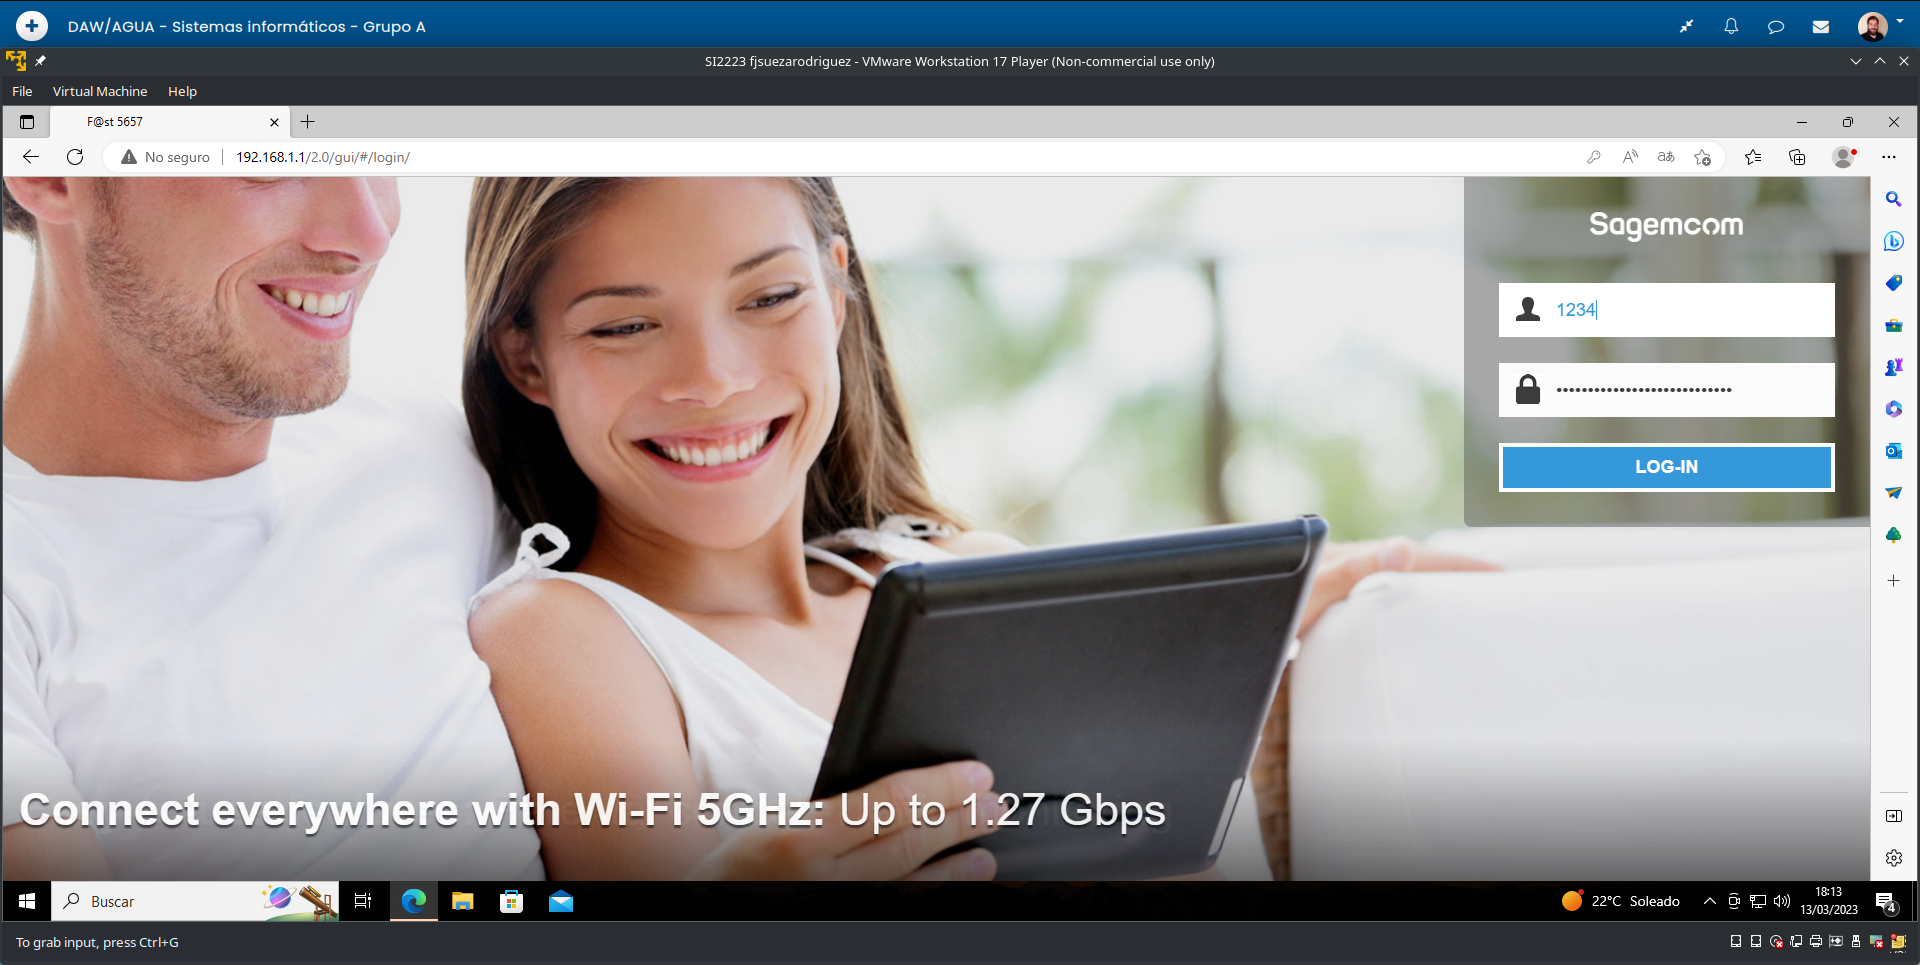
\includegraphics[scale=0.18]{router-1.png}
        \caption{Acceso al router con su interfaz web}
    \end{figure}

    \item El siguiente paso es sería cambiar la \textbf{contraseña de acceso} al router. En este ruter, hay que pulsar en la opción \textbf{Access Control} y después en la pestaña \textbf{User}, lo que nos desplegará un formulario con el que podremos cambiar la contraseña de acceso.

    \begin{figure}[H]
        \centering
        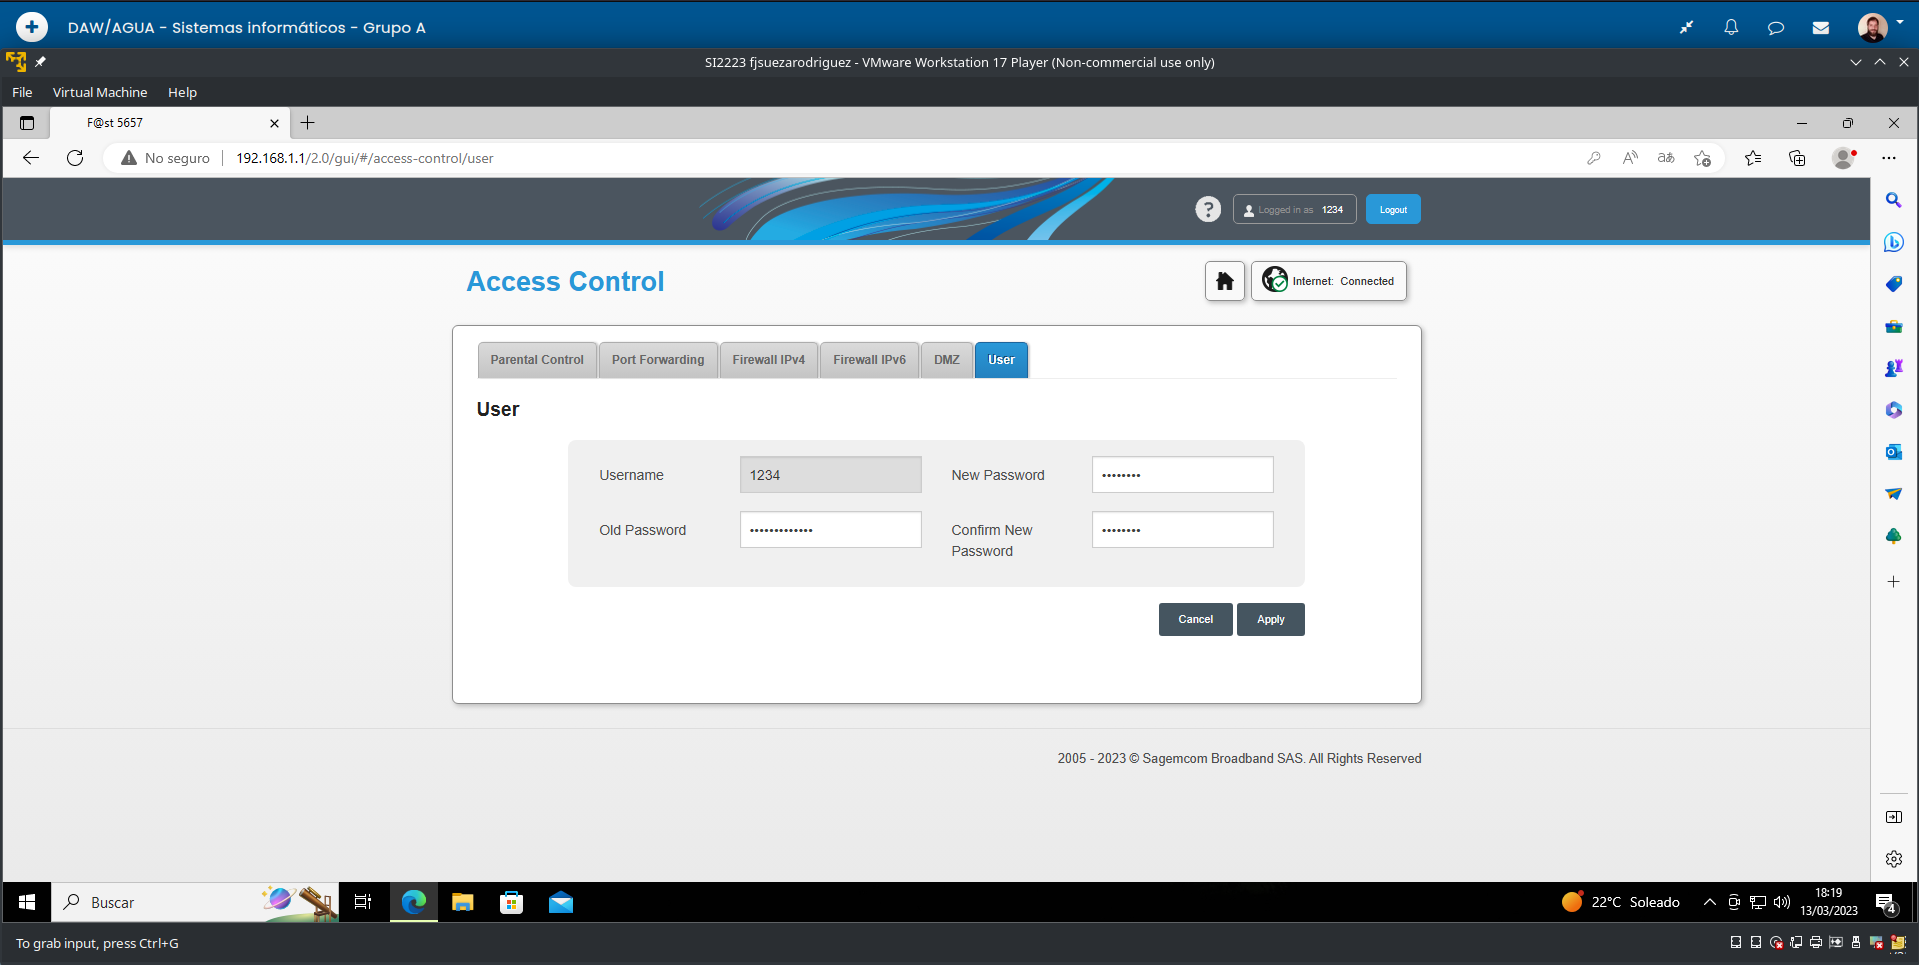
\includegraphics[scale=0.18]{router-2.png}
        \caption{Cambio de contraseña de acceso al router}
    \end{figure}

    \item A continuación vamos a cambiar la \textbf{contraseña de la red inalámbrica}. Para cambiarla, debemos pulsar en el \textbf{icono de una rueda} que aparece en la interfaz principal, al lado del nombre de la red. En la siguiente imagen, se muestra dicho icono, que también servirá para futuros pasos.

    \begin{figure}[H]
        \centering
        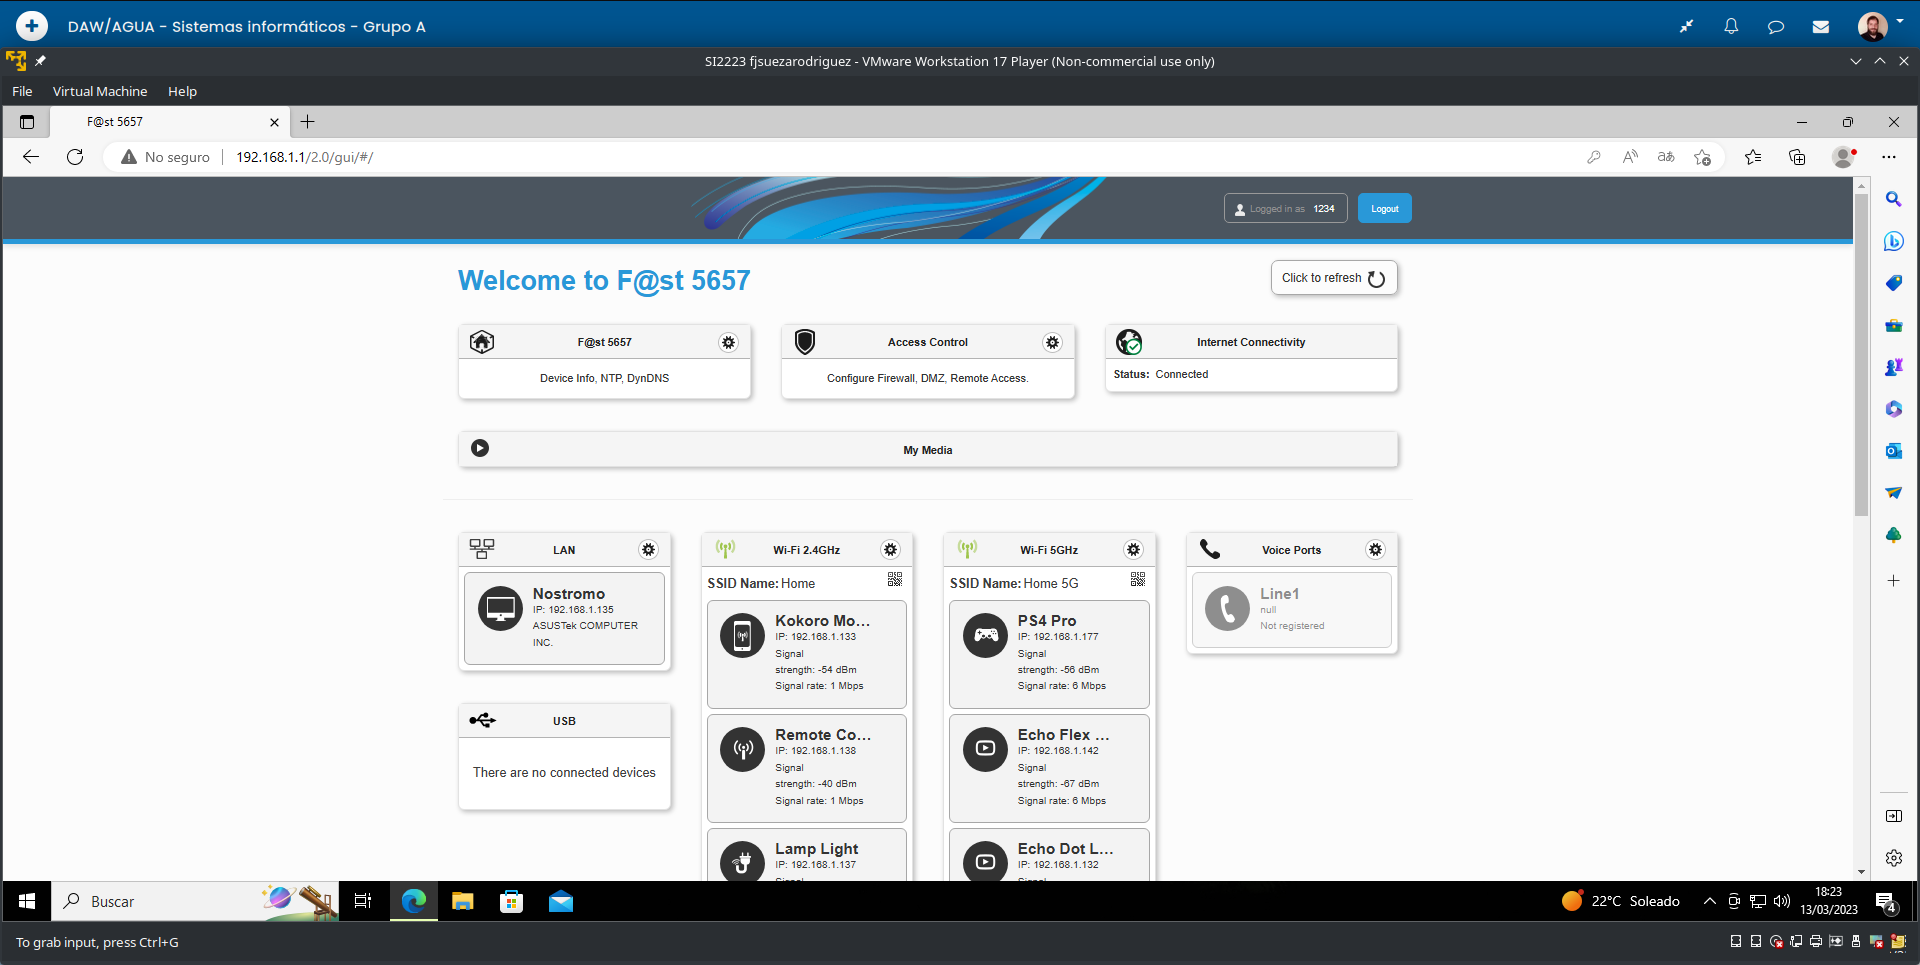
\includegraphics[scale=0.18]{router-3.png}
        \caption{Interfaz principal del router}
    \end{figure}

    En la ventana que se nos carga, en la parte inferior, podemos \textbf{cambiar la contraseña de la red}. Si queremos, podemos establecer diferentes contraseñas para la red 2.4 Ghz y la 5Ghz.

    \begin{figure}[H]
        \centering
        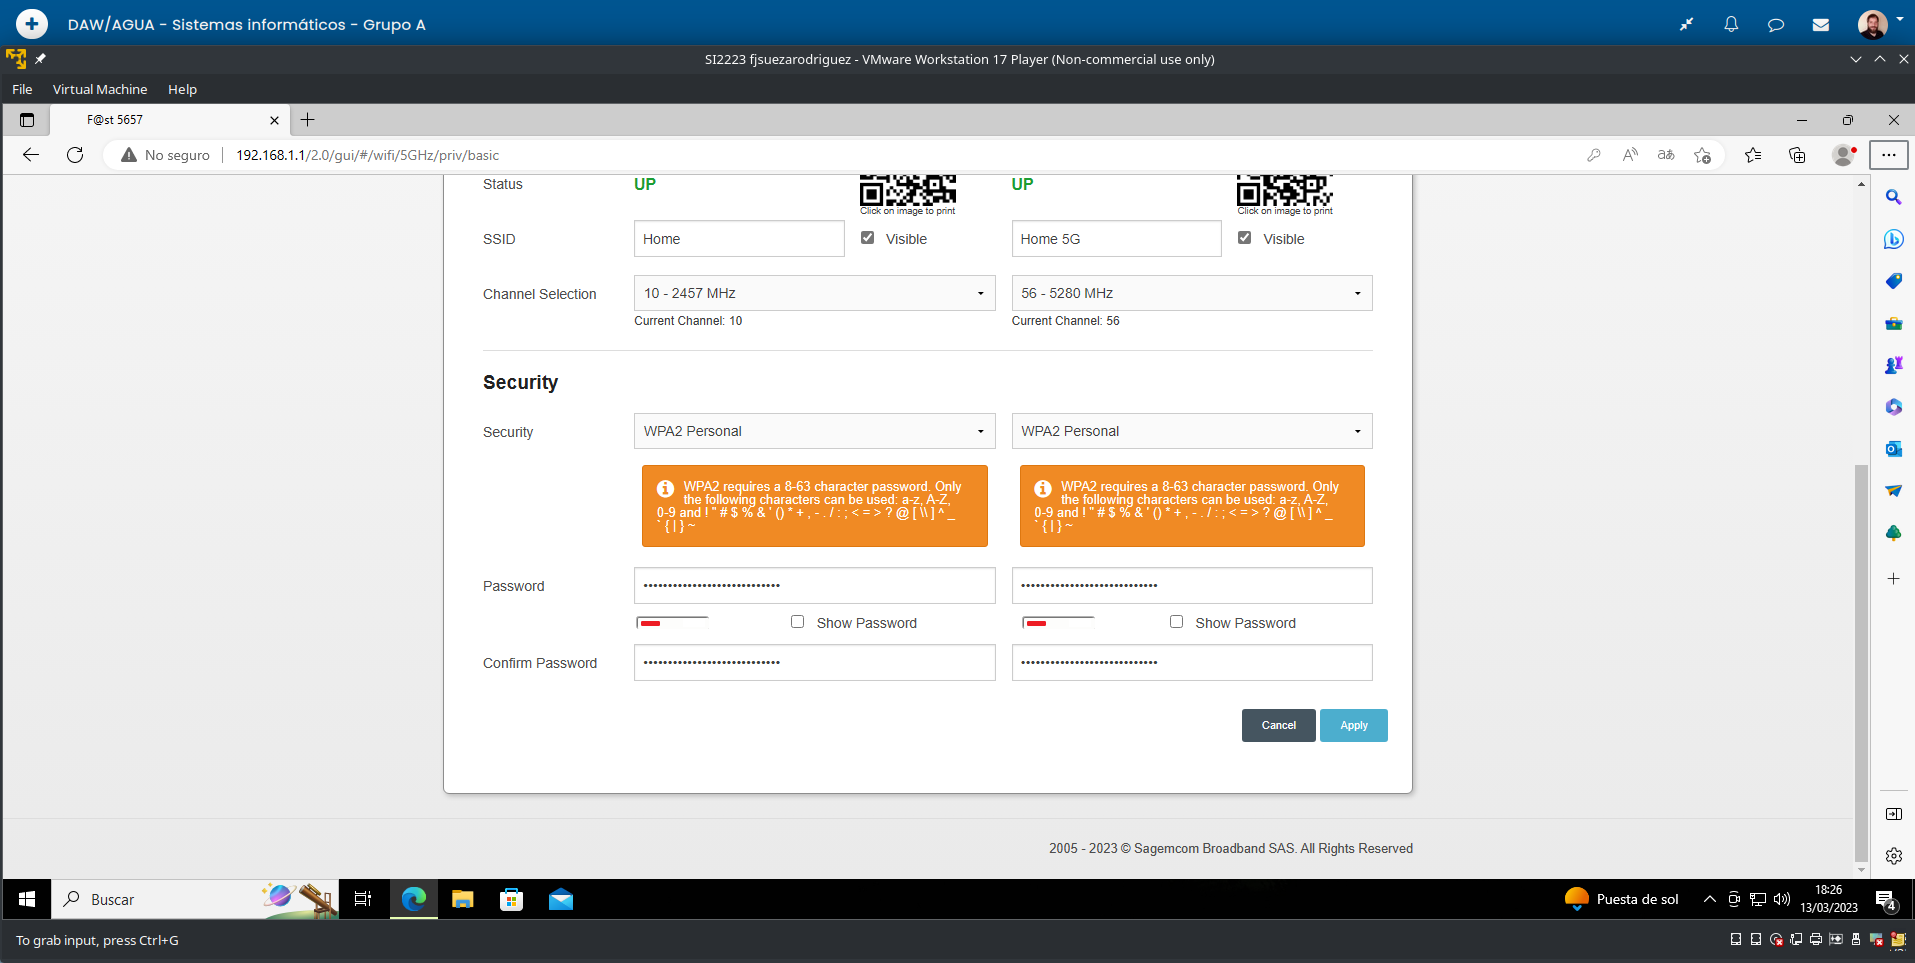
\includegraphics[scale=0.18]{router-4.png}
        \caption{Cambio de contraseña de red}
    \end{figure}

    \item En la misma ventana donde nos encontrábamos en el punto anterior, podemos cambiar el \textbf{cifrado} a \textbf{WPA2 Personal}. Como podemos ver en la siguiente captura (y en la anterior), la contraseña ya tiene es tipo de cifrado.

    \begin{figure}[H]
        \centering
        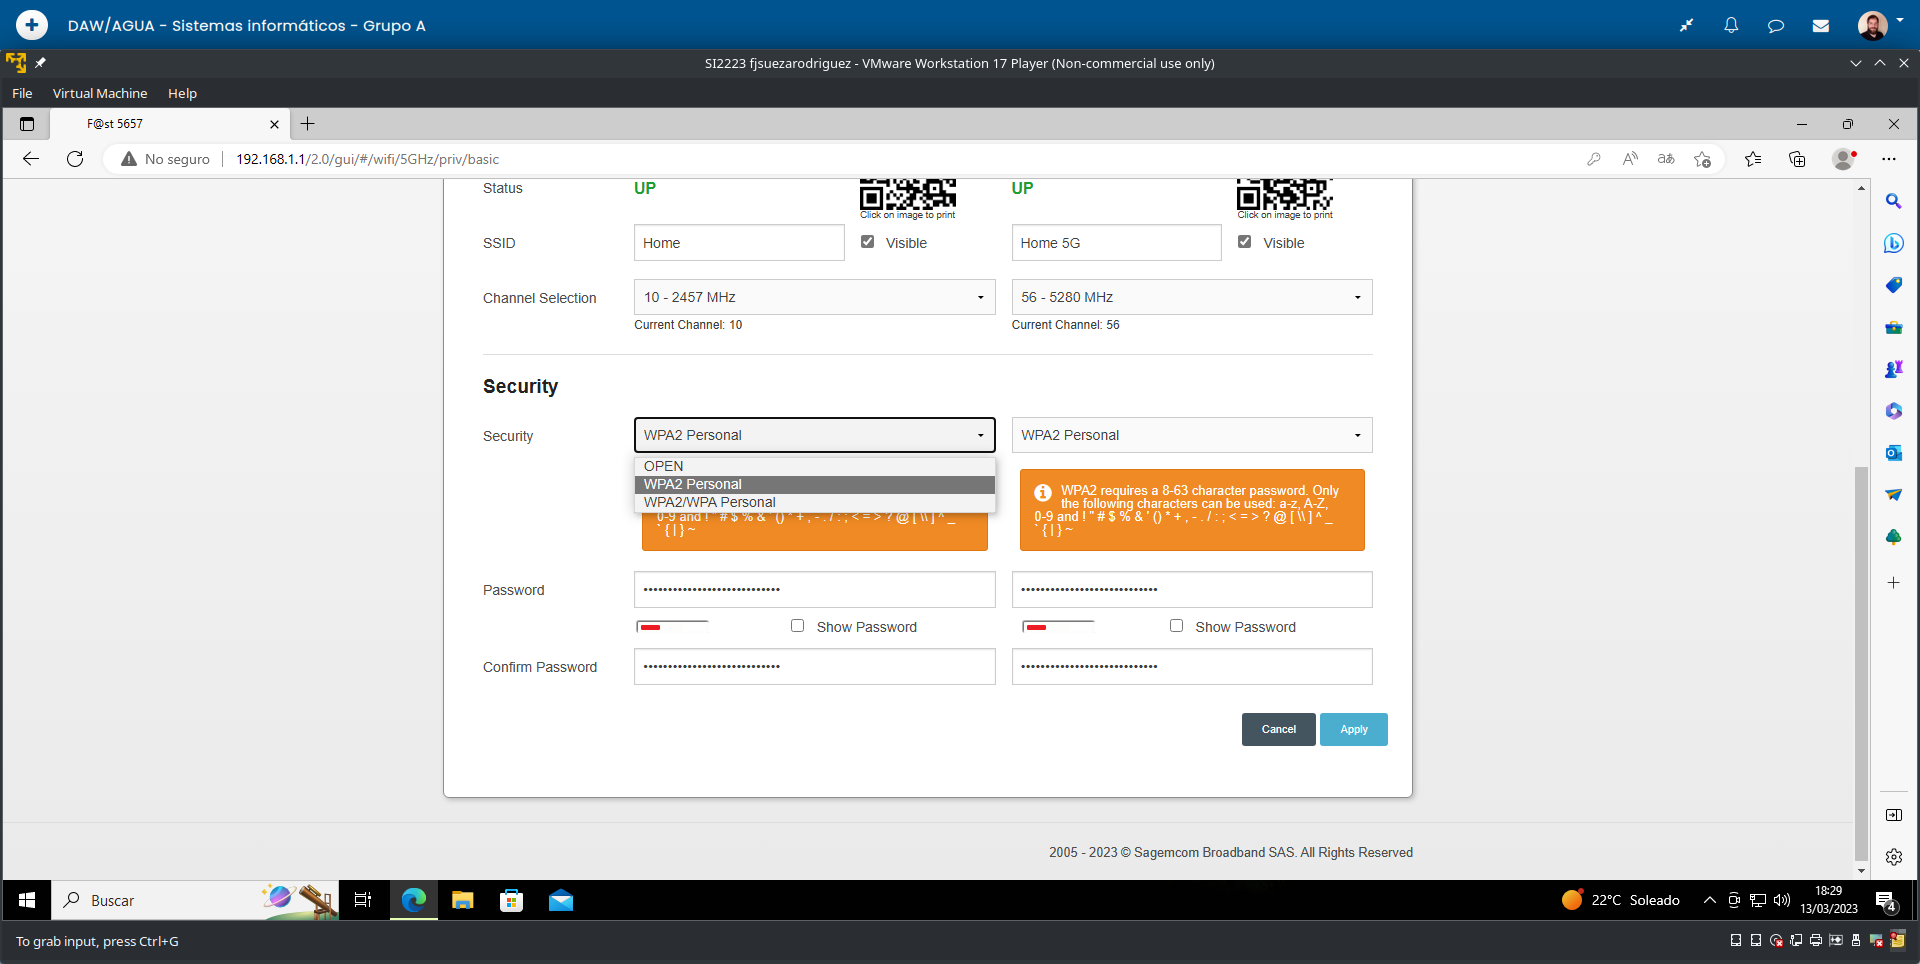
\includegraphics[scale=0.18]{router-5.png}
        \caption{Cambio del cifrado de la contraseña Wi-Fi}
    \end{figure}

    \item A continuación vamos a ver la cual es la \textbf{dirección MAC }de alguno de los dispositivos conectados a la red. Desde la \textbf{interfaz principal} del router, que hemos mostrado en la \textbf{figura 2.33}, podemos pulsar en alguno de los dispositivos que se muestran conectados a la red 2.4Ghz o a la 5Ghz. Nosotros hemos pulsado en uno y se nos muestra una pantalla con información relevante al dispositivo y su conexión con el router, entre esta información, esta la dirección MAC.

    En concreto, la dirección MAC del dispositivo elegido es \textbf{BC:CE:25:FB:B7:CC}, como vemos en la siguiente captura.

    \begin{figure}[H]
        \centering
        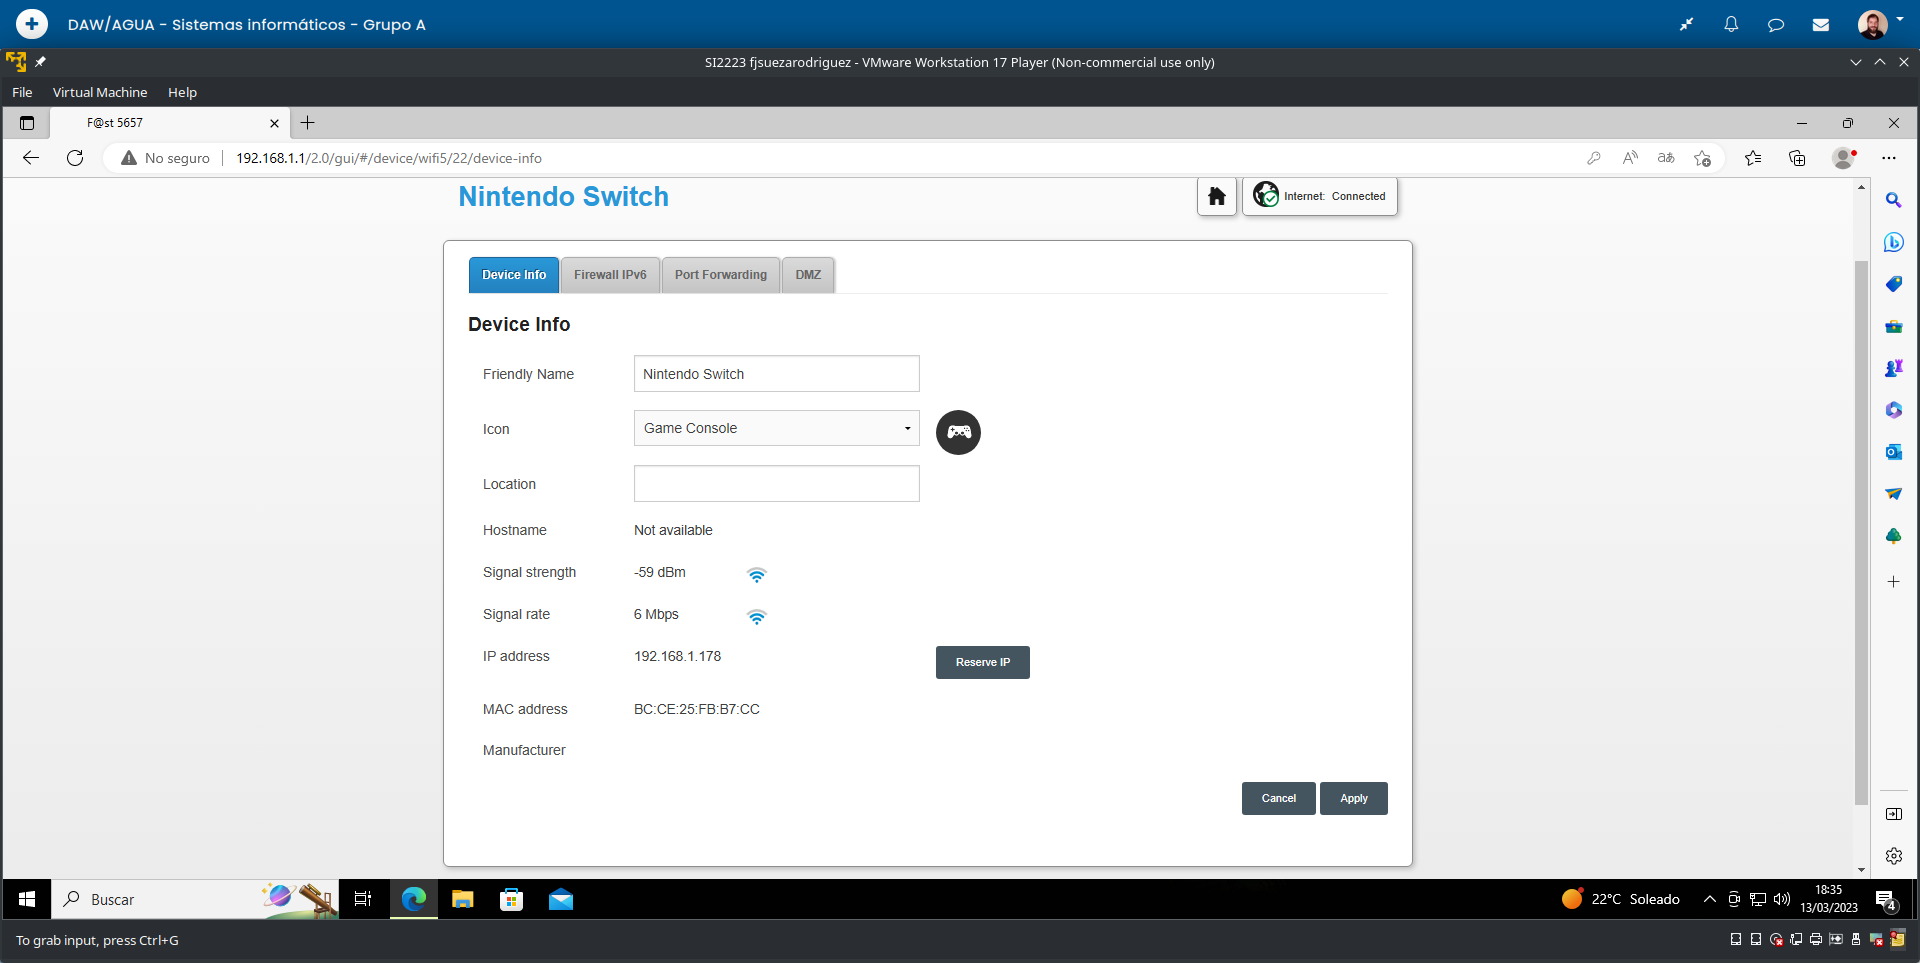
\includegraphics[scale=0.18]{router-6.png}
        \caption{Dirección MAC de un dispositivo conectado a la red}
    \end{figure}

    \item Ahora vamos a usar esa dirección en el \textbf{filtrado de direcciones MAC}. Pulsamos en el icono de la rueda, al lado del nombre de alguna de las dos redes, y en la ventana que se nos carga, en la pestaña \textbf{MAC Filter}. Aquí podemos seleccionar el modo de filtrado. Si seleccionamos \textbf{Allow All}, permitirá a cualquier dispositivo conectar. En cambio si seleccionamos \textbf{Allow} solo permitirá conectarse a los dispositivos de la tabla inferior y por último si seleccionamos \textbf{Deny}, denegará el acceso a los dispositivos introducidos.

    Nosotros hemos seleccionado \textbf{Deny} e introducido la dirección MAC del dispositivo del punto anterior.

    \begin{figure}[H]
        \centering
        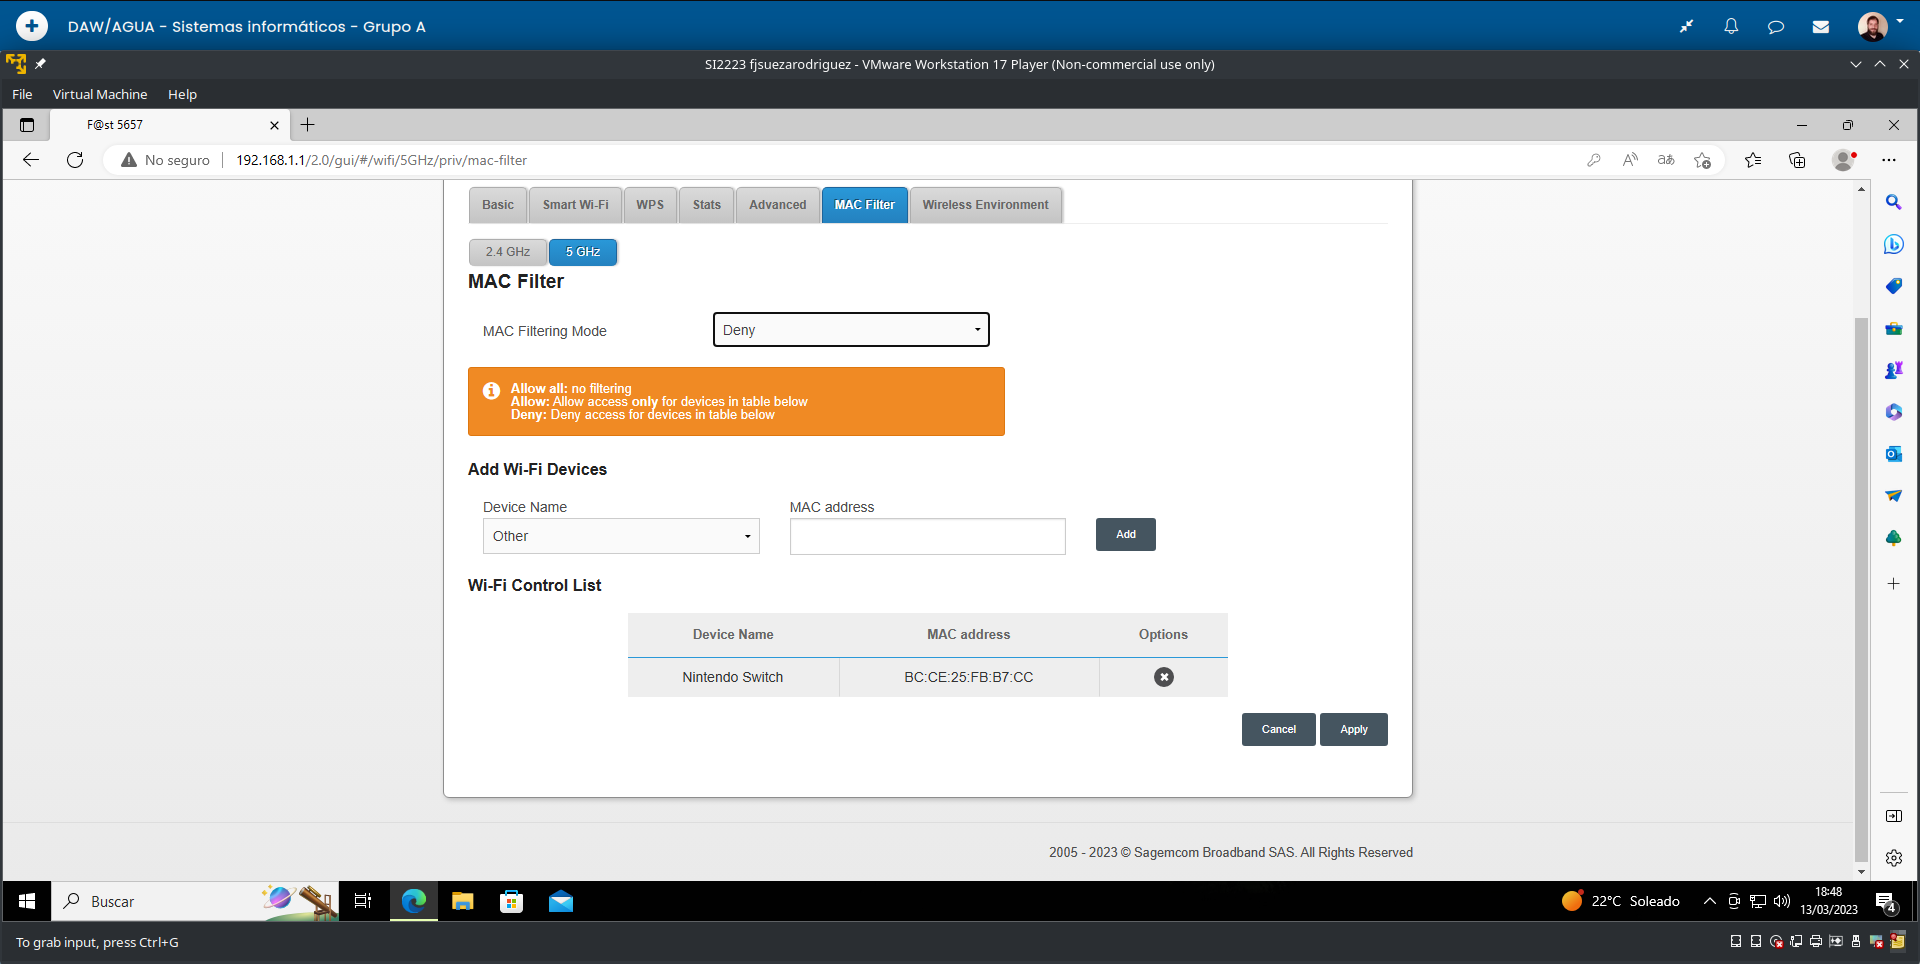
\includegraphics[scale=0.18]{router-7.png}
        \caption{Configuración del filtrado MAC}
    \end{figure}

    \item Por último,, para conectar a una red Wi-Fi, solo tenemos que pulsar en icono de red, y si tenemos una tarjeta wireless, se nos mostrará el conjunto de redes detectado, pulsamos en la red seleccionada y nos pedirá que introduzcamos los credenciales. Si los tenemos, los introducimos y podremos conectar a la red.

    \textbf{NOTA}: Esta captura esta realizada en Linux, pero el proceso es exactamente igual que en Windows.

   \begin{figure}[H]
        \centering
        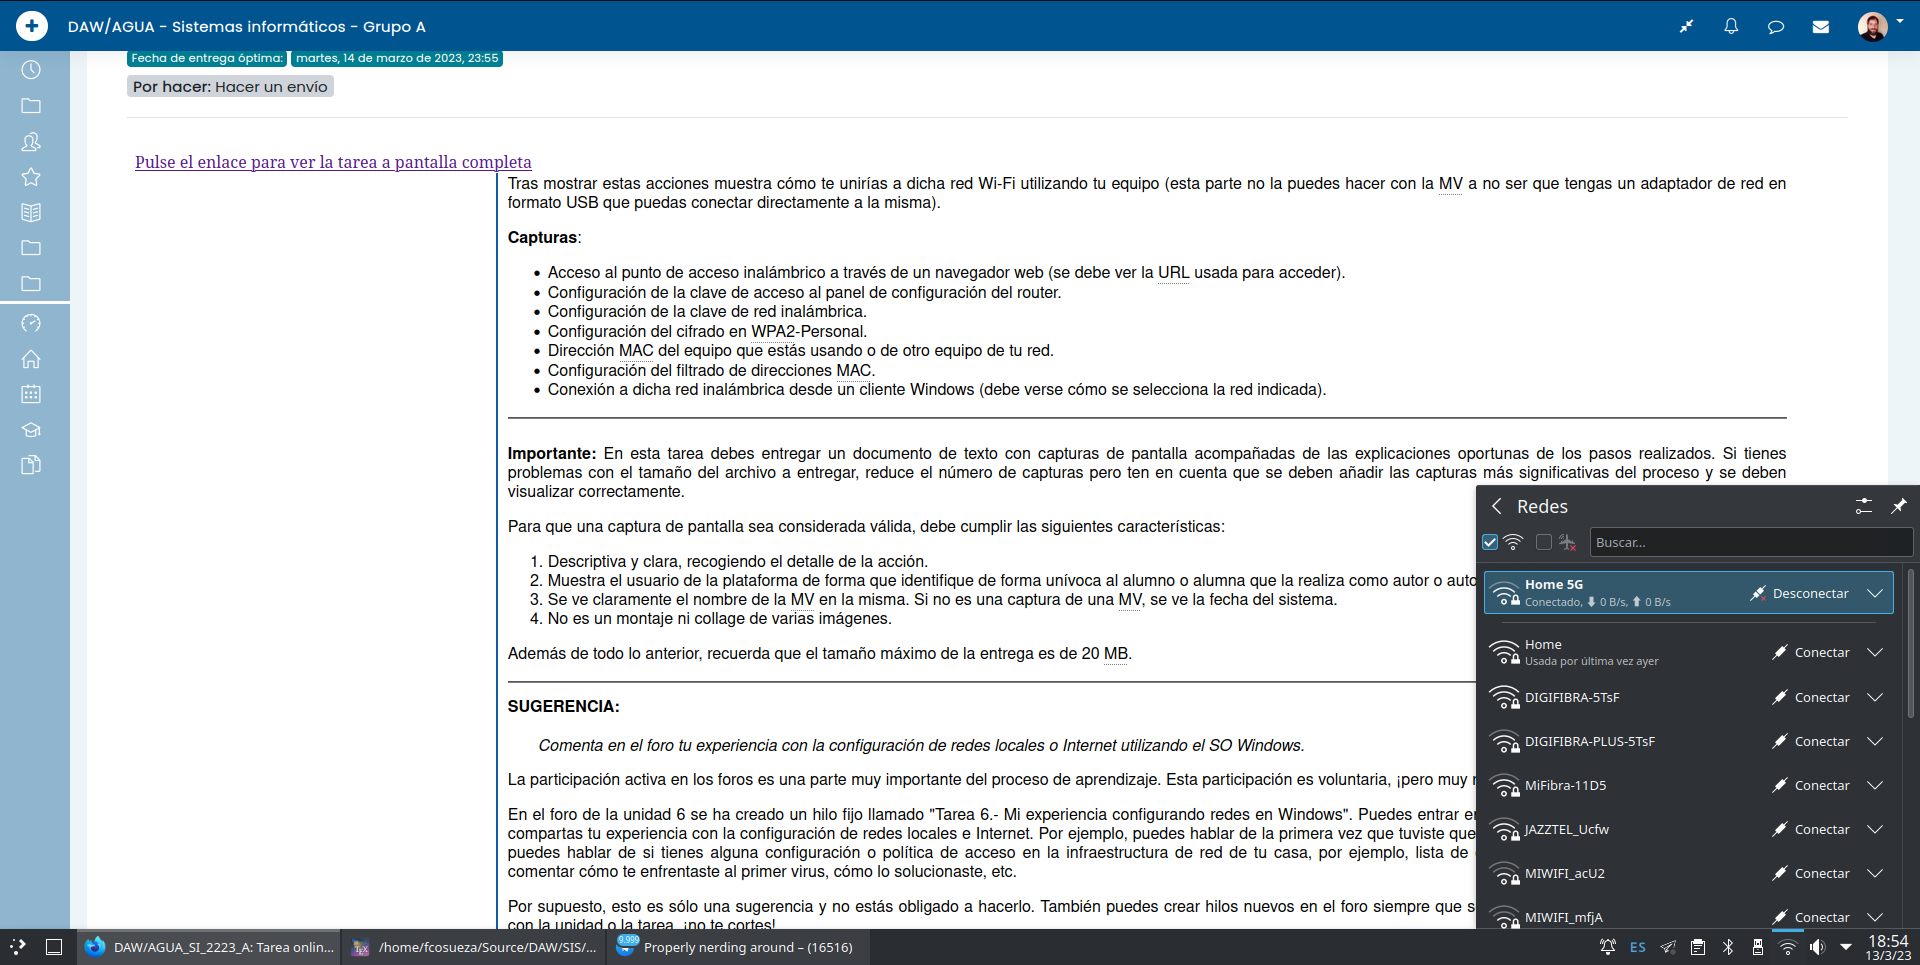
\includegraphics[scale=0.18]{router-8.png}
        \caption{Conexión a una red inalámbrica}
    \end{figure}
\end{enumerate}






% Bibliography

%\newpage
%\bibliography{citas}
%\bibliographystyle{unsrt}

\end{document}